\subsection{The impact of FCC in particle physics}
\label{sec:PhysicsCaseIntro}

Particle physics is the science of studying fundamental processes on the smallest accessible scales. 
The last sixty years of particle physics have led to a radical overhaul of the understanding of the Universe, 
culminating in the landmark discovery of the Higgs boson in 2012. 
In this context, FCC may be viewed as a general-purpose particle physics facility, aimed at completing the extensive testing of the SM, 
exploring remaining open questions, and finding leads towards understanding the fundamental origins of the Universe. 
The combination of the most powerful $\epem$ Higgs and electroweak factory with the ultimate 100\,TeV-class hadron collider 
is unique in its capacity to carry out a new phase of exploration in new regimes of precision and energy, 
and in a controlled and repeatable experimental environment. 
More specifically, FCC will shed light on the many fundamental open questions about how the Universe came to be.

\textbf{What is the origin of the Higgs boson?}  
The Higgs boson discovered at LHC, with a mass of $125.20 \pm 0.11$\,GeV, 
is, so far, consistent with the SM version of Electroweak Symmetry Breaking (EWSB), 
which predicts the full Higgs phenomenology with no free parameter. 
These predictions must be tested with the highest possible precision with FCC-ee and FCC-hh. 
Indeed, there are many reasons to believe that the underlying microscopic physics, from which the Higgs boson emerges, 
is associated with some of the deepest mysteries in particle physics.  
One such mystery concerns the origin of the Higgs boson mass and the naturalness puzzle, 
which FCC is uniquely placed to address by a combination of precision Higgs coupling measurements at the per-mil level 
and electroweak precision measurements improved by a factor of 50 or much more with respect to the current precision,
with direct high-energy exploration to comprehensively probe symmetry-based explanations for the electroweak hierarchy.

\textbf{What is the origin of the presence of matter in the Universe?} 
The predominance of matter over antimatter, a.k.a.\ the baryon asymmetry of the universe (BAU), calls for both C and CP violation, 
as well as an out-of-equilibrium epoch in cosmological history. 
The SM EWSB does not suffice to predict a significant BAU, but particle physics can propose two hypotheses to accommodate this observation. 
A first possibility is that the Higgs potential is modified via a change of the Higgs self-coupling, leading to a first-order electroweak phase transition (EWPT). 
The FCC measurement of the Higgs boson self-coupling will reach a level of precision deemed adequate to clarify 
if the EWPT played a role in setting an out-of-equilibrium phase, 
a necessary condition for creating the observed matter-antimatter asymmetry. 
Another possibility is that the Higgs boson couples to neutrinos, 
which would generate a fermion-number-violating Majorana mass term, 
leading in turn to leptogenesis and, possibly, to the right amount of BAU. 
With its very high luminosity, FCC is best suited for the direct observation of the resulting heavy neutral leptons (HNL).

\textbf{What is the origin of mass and flavour?} 
The Higgs mechanism is responsible for generating mass, but the reason for the pattern of Yukawa couplings is yet to be understood. 
The FCC unique exploration potential of flavour physics and of new symmetries and forces 
would lead to a deeper understanding of approximate conservation laws,
such as baryon and lepton number conservation 
(or the absence thereof in case of Majorana neutrinos);
would probe the limits of lepton flavour universality and violation; and 
could reveal new selection rules governing the fundamental laws of nature. 
A precise comparison of the  Yukawa couplings for the three fermion families will also be crucial in this endeavour. 
The measurements of the muon and top Yukawa couplings at FCC-hh can be compared to the tau and charm Yukawa coupling measurements at FCC-ee with sub-per-cent precision. 
A first measurement of the strange Yukawa coupling is also possible at FCC-ee. 
Finally, an FCC-ee run at the $s$-channel Higgs resonance 
uniquely offers sensitivity to the electron Yukawa coupling, tantalisingly close to its SM value.  

\textbf{What is the nature of dark matter?} 
The unprecedented luminosity and detector environment of FCC-ee make it uniquely sensitive to exploring weakly-coupled dark sectors. 
Dark matter candidates, such as heavy axions, dark photons, etc., provide long-lived particle signatures.  
If dark matter is a doublet or triplet weakly interacting massive particle (WIMP), 
FCC-hh will cover the entire parameter space up to the upper mass limit for a thermal relic. 
A range of complementary detector facilities could also be envisioned to extend the FCC capabilities for neutrino physics, long-lived particles, and forward physics.

\textbf{What lies beyond the Standard Model?} 
An impressive number of electroweak precision observables (EWPOs) will be measured by FCC-ee, 
with accuracies ranging from a factor 50 (e.g., for the \PW mass) to a factor 1000 (e.g., for $R_{\PQb}$) better than today (Table~\ref{tab:EWPO}). 
This new precision regime will allow the effect of further weakly-coupled heavy particles to be detected up to masses of several tens of TeV 
(and much more in the non-decoupling configuration). 
Alternatively, this precision will bring sensitivity to particles mixing with the SM fermions in one part in 100\,000, 
up to very high mass scales (more than 1000\,TeV for HNL). 
The SM, possibly extended with additional light degrees of freedom, 
might be a low-energy effective field theory (EFT) approximation of a microscopic, ultraviolet (UV) theory from which it originates. 
The FCC-ee will improve the sensitivity to all EFT Wilson coefficients by one to several order(s) of magnitude, 
while FCC-hh can further extend the reach of direct and indirect exploration in a complementary way. 
The combined FCC programme is the most powerful general survey of this uncharted EFT territory 
and of the existence of new particles beyond the known fermions and bosons.

\textbf{Relation with exotic astrophysical and cosmological signals} 
Stochastic gravitational waves from cosmological phase transitions or astrophysical signatures of high-energy gamma rays 
are examples of phenomena that can arise due to exotic new physics which is, by contrast, 
directly accessible only to a facility offering the highest possible energy, such as FCC. 
Examples include confining new physics in a dark sector, decaying or co-annihilating TeV-scale WIMPs, or a modified EWPT. 
More precise top quark and Higgs boson mass measurements would also have important implications in the understanding of the SM vacuum metastability.

As an all-in-one-facility, FCC provides the versatility, redundancy, and cross-correlations ne\-cessary to identify the fundamental origins of new phenomena. 
In general, its varied range of precise measurements of particle properties and interaction dynamics 
promises a set of guaranteed results with an unrivalled breadth with respect to other potential future facilities.

This chapter presents the unique role of FCC to address these fundamental questions, with a special focus on: 
the combined characterisation of the Higgs boson at FCC-ee and FCC-hh (Section~\ref{sec:PhysicsCaseHiggsEW}); 
the direct discovery potential resulting from the FCC-ee clean environment, high integrated luminosity, and large acceptance rates of the detectors (Section~\ref{sec:PhysicsCaseBSM}); 
and the excellent opportunities in flavour physics (Section~\ref{sec:PhysicsCaseFlavour}). 
The advantages of FCC-hh over multi-TeV lepton colliders to complement FCC-ee are presented in Section~\ref{sec:PhysicsCaseHHvsHEL}. 
Finally, the physics reach of FCC-hh as a function of its centre-of-mass energy, 
and the possibility of a forward-physics facility at FCC-hh, 
are briefly discussed in Sections~\ref{sec:PhysicsCaseHHscenarios} and~\ref{sec:PhysicsCaseHHFPF}.

\subsection{Characterisation of the Higgs boson: role of EW measurements and of FCC-hh}
\label{sec:PhysicsCaseHiggsEW}

The Higgs boson is certainly a central piece of the current understanding of the fundamental structure of matter and physics laws. 
Its discovery in 2012, and the rich measurement programme over the past thirteen years, 
have been successful milestones in high-energy physics that, maybe more importantly, 
enabled the formulation of relevant questions about the nature of new physics beyond the weak scale, 
in very concrete and often quantitative terms. 
As already shown in various studies~\cite{deBlas:2019rxi, DeBlas:2019qco, deBlas:2022ofj}, 
FCC-ee offers fantastic opportunities for learning more about the Higgs boson, 
beyond what can be achieved at HL-LHC (Table~\ref{tab:HiggsKappa3}) or at other proposed Higgs factories~\cite{Blondel:2024mry}.


\begin{table}[ht]
\centering
\caption{Expected 68\%~CL relative precision of the $\kappa$ parameters (Higgs couplings relative to the SM) 
and of the Higgs boson total decay width $\Gamma_{\PH}$, 
together with the corresponding 95\%~CL upper limits on the untagged (undetected events), $\cal{B}_{\text{unt}}$, 
and invisible, $\cal{B}_{\text{inv}}$, branching ratios at HL-LHC, FCC-ee (combined with HL-LHC), and the FCC integrated programme.
For the HL-LHC numbers, a $|\kappa_V| \leq 1$ constraint is applied (denoted with an asterisk), 
since no direct access to $\Gamma_{\PH}$
is possible at hadron colliders;
this restriction is lifted in the combination with FCC-ee.
The `--' indicates that a particular parameter has been fixed to the SM value, due to lack of sensitivity.
From Ref.~\cite{deBlas:2019rxi}, updated with 4~IPs, the baseline luminosities of Table~\ref{tab:seqbaseline}, and the most recent versions of the data analysis. 
For some of the entries, the $\kappa$ precision starts being limited by the projected SM parametric uncertainties, e.g. in $m_{\PQb}$~\cite{Freitas:2019bre}. For these entries, the precision obtained by neglecting such parametric uncertainties is also reported (separated by a $/$).
}
\label{tab:HiggsKappa3}
\begin{tabular}{ c   c    c     c }%| c }
\toprule
Coupling & HL-LHC 
& FCC-ee 
& FCC-ee $+$ FCC-hh\\ 
\midrule 
$\kappa_{\PZ}$ (\%) &  1.3$^\ast$ 
& 0.10  
& 0.10 \\ 
$\kappa_{\PW}$ (\%)  &   1.5$^\ast$  
& 0.29 
& 0.25 \\
$\kappa_{\PQb}$ (\%)  & 2.5$^\ast$  
& 0.38 / 0.49 
& 0.33 / 0.45 \\ 
$\kappa_{\Pg}$ (\%)    &   2$^\ast$ 
& 0.49 / 0.54 
& 0.41 / 0.44 \\
$\kappa_{\PGt}$ (\%)   & 1.6$^\ast$   
& 0.46 
& 0.40 \\
$\kappa_{\PQc}$ (\%)   & --  
&0.70 / 0.87 
& 0.68 / 0.85 \\
$\kappa_{\PGg}$ (\%)  &  1.6$^\ast$  
& 1.1 
& 0.30 \\
$\kappa_{\PZ\PGg}$ (\%)    & 10$^\ast$  
& 4.3
& 0.67\\
$\kappa_{\PQt}$ (\%)   & 3.2$^\ast$ % & 3.1
& 3.1 
& 0.75 \\
$\kappa_{\PGm}$ (\%)     & 4.4$^\ast$  
& 3.3 
& 0.42 \\
$\vert \kappa_{\PQs}\vert$ (\%) & -- & $_{-67}^{+29}$ & $_{-67}^{+29}$\\
$\Gamma_{\PH}$ (\%) & -- 
& 0.78
& 0.69 \\ 
$\cal{B}_{\text{inv}}$ ($<$, 95\% CL) 
& $1.9 \times 10^{-2}$ $^\ast$   
& $5 \times 10^{-4}$ 
& $2.3 \times 10^{-4}$ \\
$\cal{B}_{\text{unt}}$ ($<$, 95\% CL) & $4 \times 10^{-2}$ $^\ast$ 
& $6.8\times 10^{-3}$ 
& $6.7\times 10^{-3}$\\
\bottomrule
\end{tabular}
\end{table}


In a record time, FCC-ee will bring the Higgs programme into a sub-percent precision area, 
allowing the classical as well as the quantum mechanical effects of new physics on the Higgs couplings to be probed and, 
from the pattern of the deviations, new selection rules distinguishing different models to be discovered. 
Concrete examples proving the relevance of the sub-percent precision target can be found in Table~5 of Ref.~\cite{Barklow:2017suo}, 
where several BSM models beyond the reach for direct discovery at HL-LHC are considered, 
and for which per-cent level deviations in the Higgs couplings are predicted. 
A sub-per-cent precision is a clear necessary target to expose such deviations.
As mentioned in Section~\ref{sec:overview_ee}, the Higgs precision programme at 240\,GeV (365\,GeV) 
can be achieved within three (eight) years of operation with FCC-ee, 
while other colliders considered at CERN would need half a century to reach a similar precision~\cite{Blondel:2024mry}.

These phenomenological projections are now being confirmed by independent experimental studies, 
with different detector set-ups~\cite{HiggsNoteRecoil, note_Higgs_to_hadrons, HiggsInvisibleNote}. 
Further directions in the Higgs precision programme also need to be more systematically investigated beyond what was done so far, 
in particular in the context of specific flavour scenarios or considering BSM sources of CP violation. 
This document, instead, emphasises the benefit of the interplay between Higgs and electroweak measurements, 
a specificity of FCC-ee that was not discussed in detail in the FCC CDR~\cite{fcc-phys-cdr, fcc-ee-cdr} 
and has been studied afterwards~\cite{DeBlas:2019qco, deBlas:2022ofj}.

The interpretation of current Higgs boson measurements at LHC is so far not hindered by the limited precision of the electroweak measurements at LEP and SLC. 
With FCC-ee targeting an order-of-magnitude improvement in the precision of Higgs boson properties in the main channels, 
the current (experimental and theoretical) precision on electroweak quantities would become a limitation. 
The \PZ-pole run of FCC-ee is instrumental in avoiding contamination from electroweak coupling uncertainties in the Higgs boson characterisation. 
If the electroweak symmetry is linearly realised in the SM fields, 
the interplay between the Higgs and electroweak sectors is even deeper~\cite{Gupta:2014rxa}.
Indeed, $\epem \to \PWp\PWm$ production is then sensitive to some of the same new-physics effects as Higgs boson production and decay processes, 
making both types of measurements complementary.

The Standard Model Effective Field Theory (SMEFT) framework  is adopted, truncated to operators of dimension six~\cite{Buchmuller:1985jz, Grzadkowski:2010es}. 
The SMEFT is an appropriate framework for enumerating and quantifying the different possibilities in a relatively model-independent way. 
It assumes that new physics arises at a scale $\Lambda$, significantly above the electroweak scale, with the Higgs boson embedded in a $\text{SU}(2)_L$ doublet. 
The current status of the global SMEFT fit is shown in Fig.~\ref{fig:Global_Fit}, adapted from Ref.~\cite{deBlas:2022ofj}. 
%
In this figure, the results of the fit for the different dimension-six operators 
affecting at leading order either the electroweak processes 
(including anomalous triple gauge couplings, aTGCs, and boson-fermion couplings, Vff)  
or the Higgs processes, or both simultaneously, 
are projected on a more physically meaningful set of effective couplings capturing the effects of new physics.
%
More details can be found in Ref.~\cite{deBlas:2022ofj}.

\begin{figure}[t]
\centering
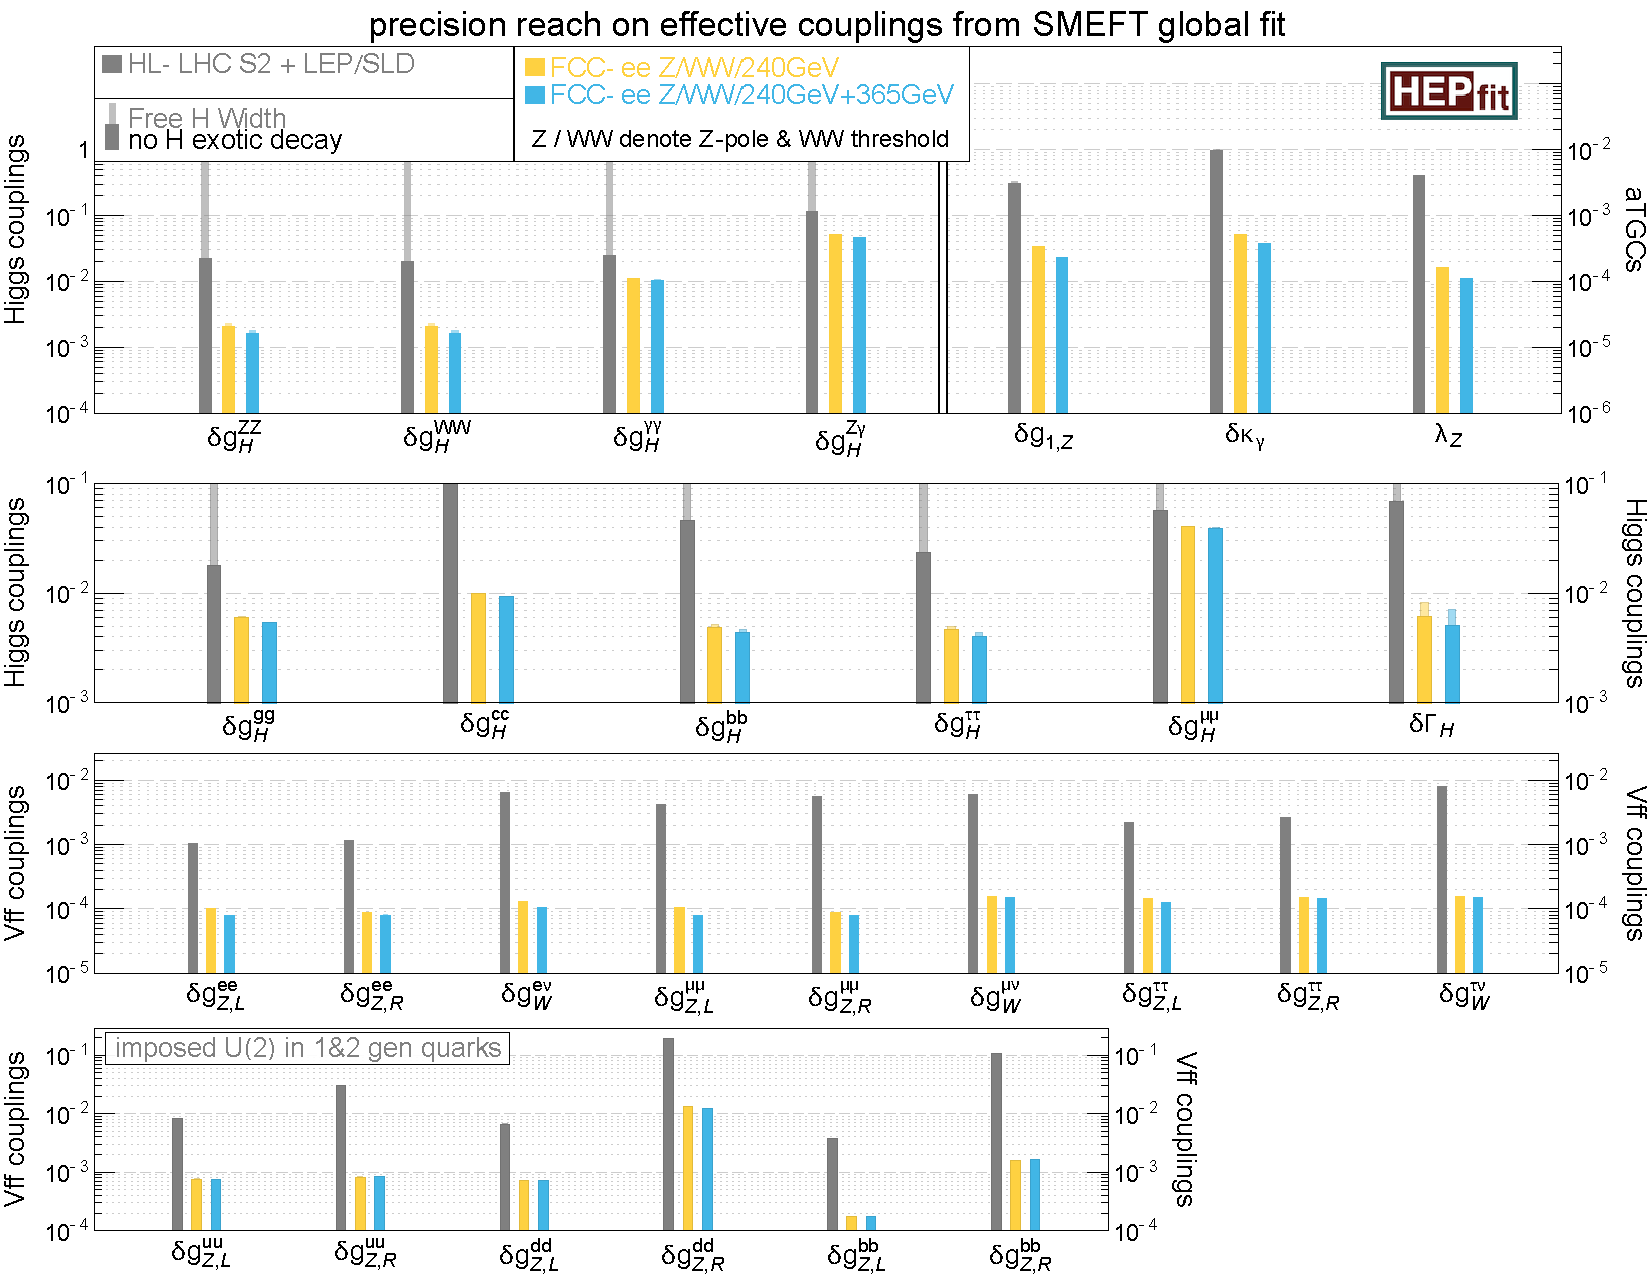
\includegraphics[width=0.95\textwidth]{PhysicsCase/Figs/barplotsnow-xo1-smpar_newFSR-CL.pdf}
\caption{Results of a global SMEFT fit to HL-LHC (grey) and FCC-ee (yellow, up to 240\,GeV, and blue, up to 365\,GeV) data, 
interpreted in terms of the 68\% probability sensitivity to Higgs and electroweak effective couplings. 
Adapted from Ref.~\cite{deBlas:2022ofj}.}
\label{fig:Global_Fit}
\end{figure}

The interplay between Higgs and electroweak measurements is illustrated in Fig.~\ref{fig:Corr_Plot}, 
which shows the expected precision in the effective coupling determination. 
The correlations are displayed as internal lines of variable thickness and are visibly reduced 
when including \PZ-pole data at FCC-ee (dark blue) on top of the current electroweak measurements (light blue). 
The importance of \PZ-pole measurements is summarised below, followed by a discussion of the importance of the diboson process for Higgs physics.

\begin{figure}[ht]
\centering
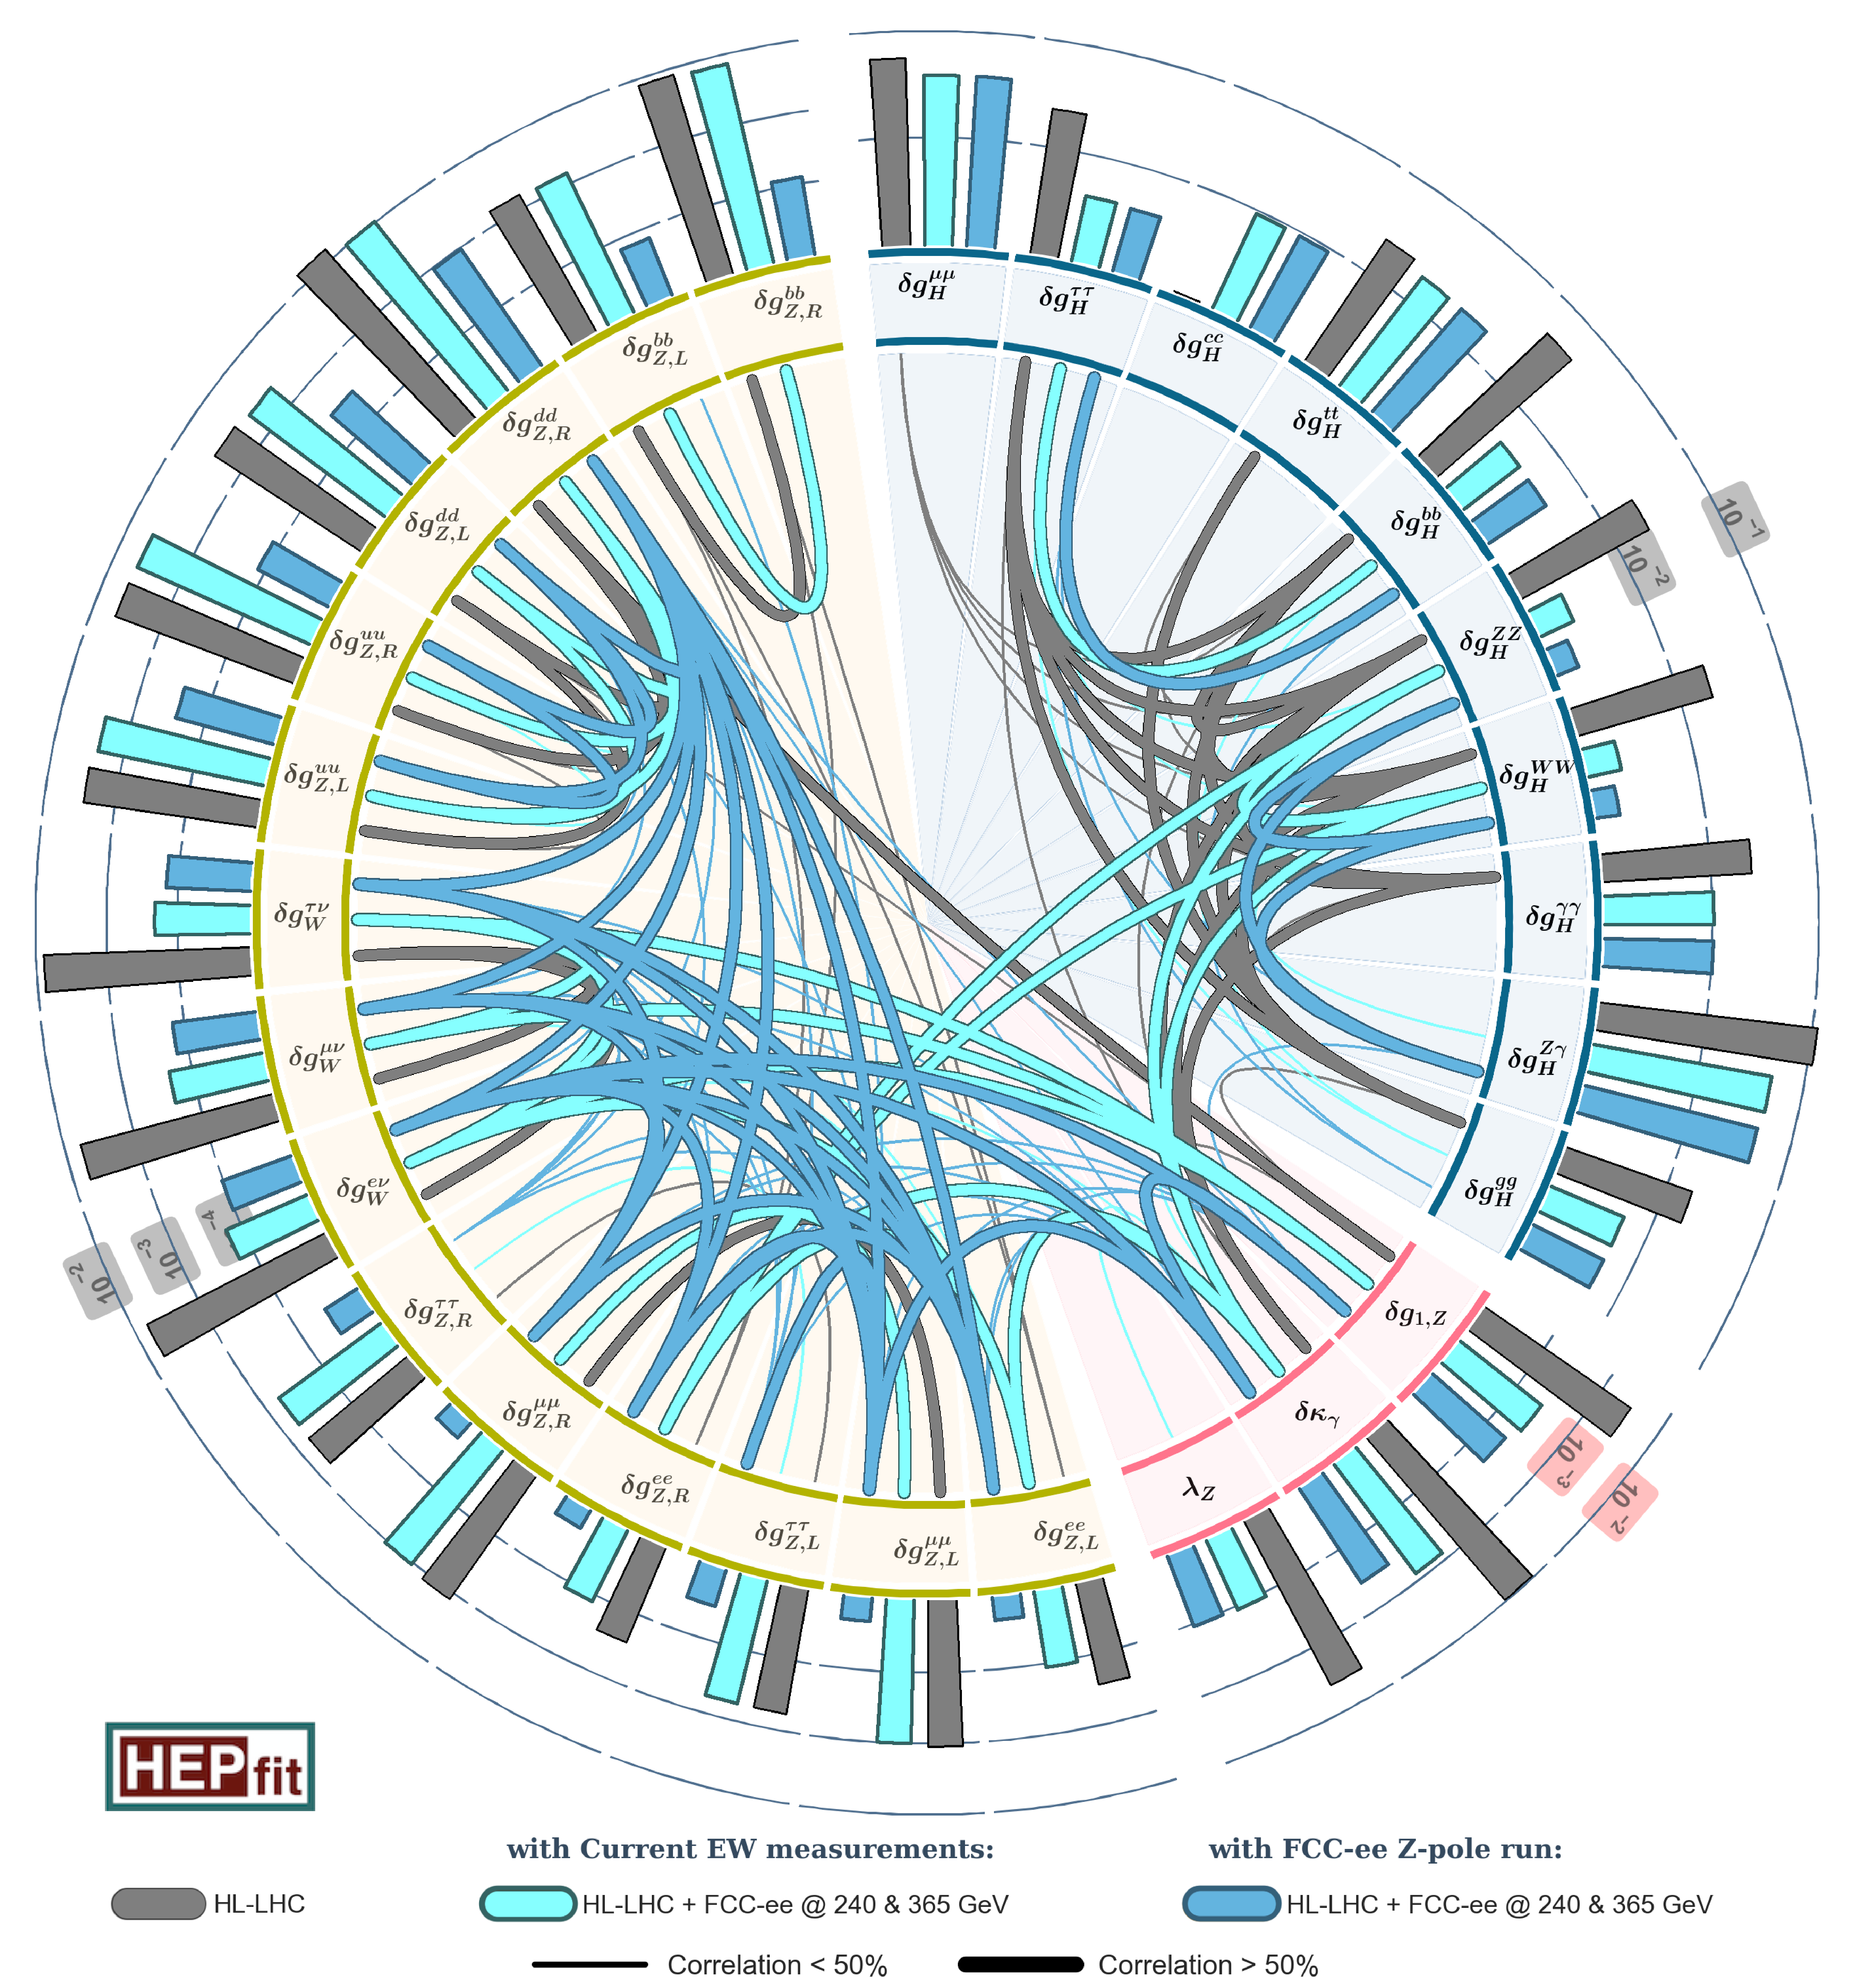
\includegraphics[width=0.80\textwidth]{PhysicsCase/Figs/circos_FCCee_nomargin_newFSR.pdf}
\caption{Correlations between the determination of different EW/aTGC/Higgs interactions from a fit to future projections at HL-LHC and FCC-ee within the SMEFT framework. 
The bars on the exterior of the circle indicate the expected sensitivity in the determination of corresponding coupling (with different scales for the different sectors). 
The light/dark blue lines in the interior of the circle show the results excluding/including the FCC-ee programme of EW measurements at the \PZ pole. 
The \PZ-pole run is essential to isolate the Higgs measurements (there is no dark blue line connecting the Higgs and EW sectors) 
and to ensure that the extraction of the Higgs couplings is not hindered by the uncertainties on the EW coupling determination.
Adapted from Refs.~\cite{DeBlas:2019qco,deBlas:2022ofj}.}
\label{fig:Corr_Plot}
\end{figure}

The SMEFT results discussed in this section were obtained from fits with only linear effects in $\Lambda^{-2}$, consistently with the dimension-6 expansion. 
To estimate the theory uncertainty associated with the neglected higher-order terms in the EFT expansion, 
Fig.~\ref{fig:ImpactQuad_Plot} shows the ratio of the bounds on the Wilson coefficients obtained in the linear case 
to those including quadratic contributions from dimension-6 operators, 
which are formally of the same order as dimension-8 contributions. 
These results derive from the HL-LHC$+$FCC-ee SMEFT fit of Ref.~\cite{Celada:2024mcf}.
All the displayed operator coefficients can be accessed at FCC-ee, with the exception of the operators in the top-left quadrant, 
which enter in top-quark measurements at HL-LHC but do not contribute to FCC-ee observables at tree level. 
So, in almost all cases, the results of the linear fit are unchanged after the addition of quadratic effects. 
This observation can be used as an indication that the uncertainty associated to effects of ${\cal O}(\Lambda^{-4})$ is well controlled 
by FCC-ee precision measurements and is expected to be small. 
Another way to gauge the usefulness of the SMEFT analysis is to 
compare the bound on the scale of new physics inferred from the fit of the dimension-6 Wilson coefficients 
to the actual limits set in explicit BSM models, as will be reported in the next section. 
Of course, this does not exclude that (non-decoupling) new physics could still exist at much lower scales.

\begin{figure}[ht]
\centering
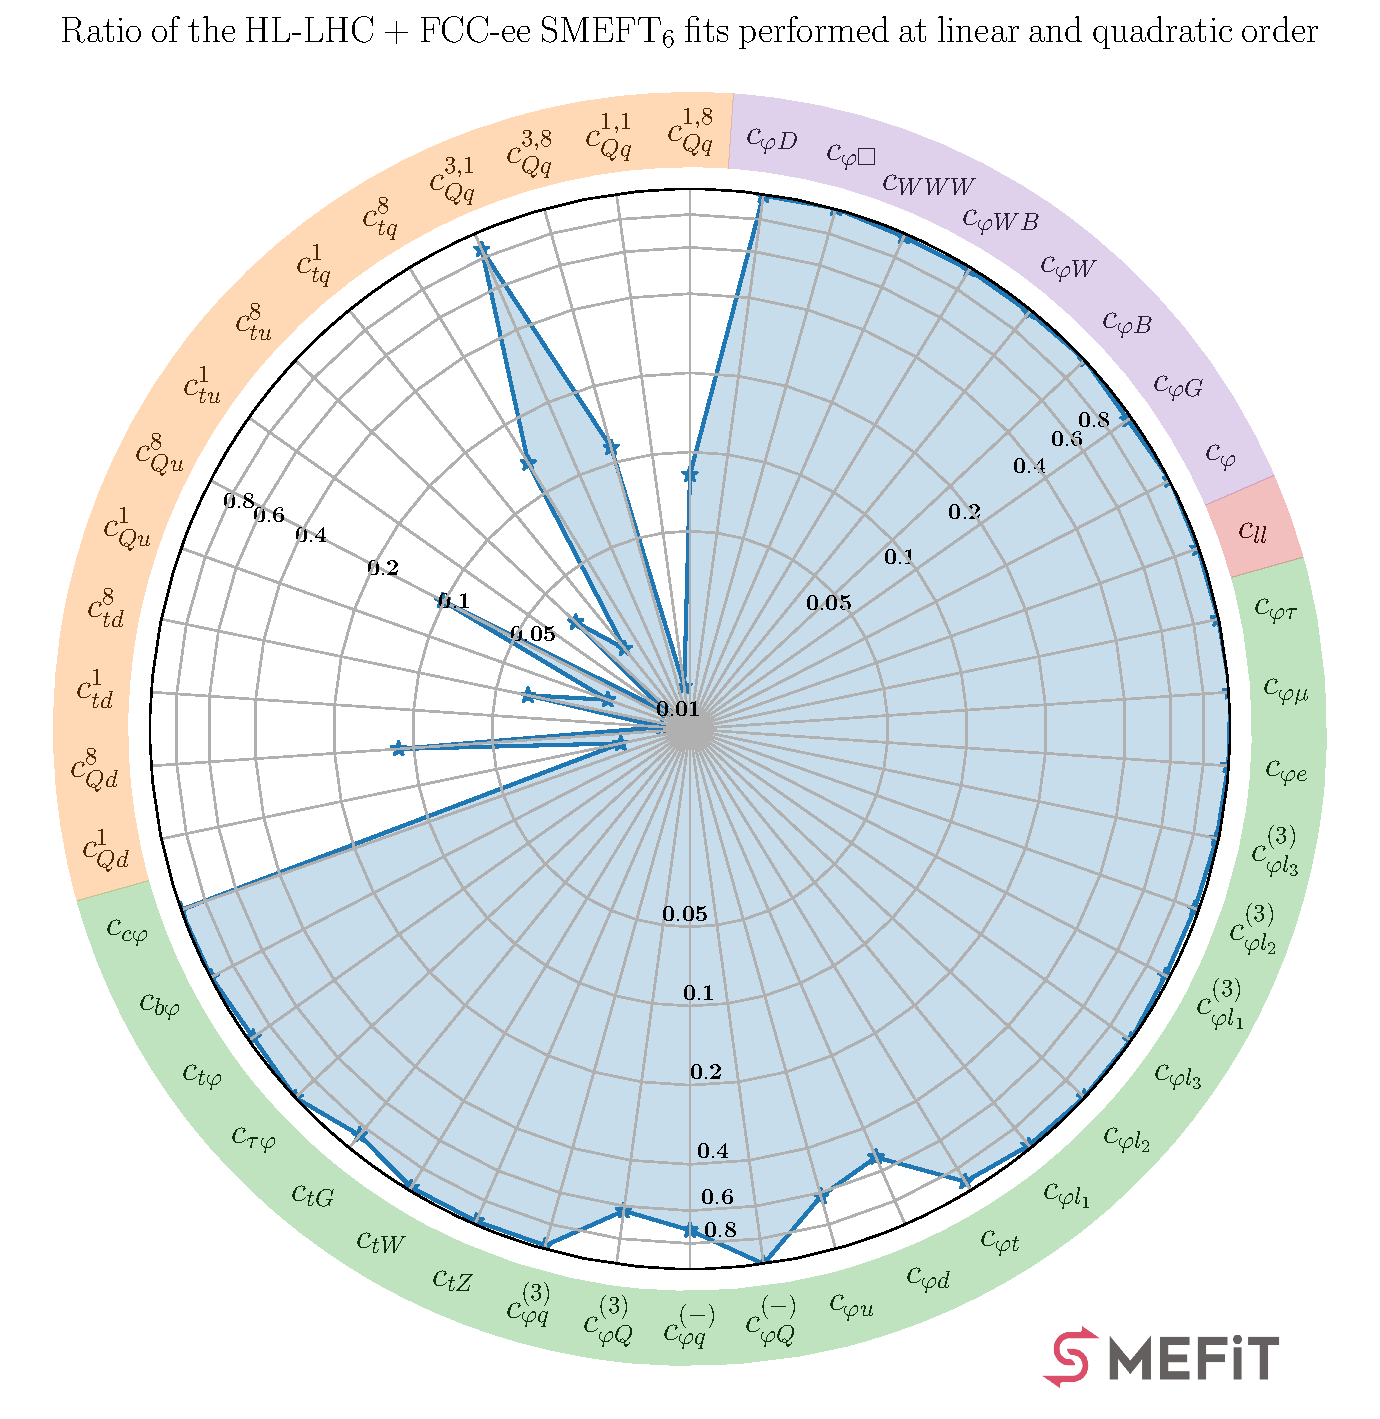
\includegraphics[width=0.80\textwidth]{Physics/PhysicsCase/Figs/spider_plot_SMEFiT_FCCFeasRep_FSR.pdf}
\caption{Impact of quadratic contributions from dimension-6 operators, i.e., at ${\cal O}(\Lambda^{-4})$, in the SMEFT fit of Ref.~\cite{Celada:2024mcf}. 
A $U(2)_Q \times U(2)_u \times U(3)_d \times \left( U(1)_L \times U(1)_e \right)^3$ flavour symmetry is assumed. 
For each of the different Wilson coefficients considered, 
the blue star indicates the ratio of the bound obtained in the pure dimension-6 (linear) fit to that including quadratic dimension-six contributions. 
The difference between the two fits is minimal for most operators entering in FCC-ee observables at tree level, 
i.e., leaving aside the purely hadronic top-quark operators in the top-left quadrant. The FCC-ee fit includes EWPOs at the $\PZ$-pole, light fermion-pair production, Higgs boson production ($\PZ\PH +$ VBF), diboson production, and top pair production.}

\label{fig:ImpactQuad_Plot}
\end{figure}

\subsubsection{Impact of \texorpdfstring{\PZ}{Z}-pole measurements in Higgs couplings determination}

The importance of having precise \PZ-pole measurements for the extraction of Higgs couplings from future $\epem$ Higgs data is clear, 
given that the $\PZ\Pe\Pe$ vertex also enters in $\PZ\PH$ production. 
A precise-enough extraction of the $\PZ\Pe\Pe$ vertex is therefore needed to avoid extra uncertainties from new physics effects in these interactions. The left-handed and right-handed $\PZ\Pe\Pe$ couplings can be extracted from the $\PZ \to \epem$ partial decay width and the left-right asymmetry parameter $A_{\rm e}$, determined at FCC-ee from the hadronic-to-leptonic cross-section ratios, the dilepton forward-backward asymmetries, and the tau polarisation forward-backward asymmetry, measured at the Z pole. This $\PZ\Pe\Pe$ coupling measurement also helps mitigating the (centre-of-mass-energy growing) new-physics effects in the $\PH\PZ\Pe\Pe$ interactions, 
directly correlated with the new-physics contributions to the $\PZ\Pe\Pe$ vertex in the SMEFT formalism.

The impact of \PZ-pole measurements in Higgs coupling fits was studied in Ref.~\cite{DeBlas:2019qco} and, more recently, in Ref.~\cite{deBlas:2022ofj}. 
As a result of the reduced correlations between the $\PH\PZ\PZ$ and $\PZ\Pe\Pe$ couplings, displayed in Fig.~\ref{fig:Corr_Plot}, 
and of the corresponding reduction of the uncertainty in the $(\PH)\PZ\Pe\Pe$ interactions, 
the precision of the extraction of the Higgs couplings is improved, 
as illustrated in Fig.~\ref{fig:ZpoleHiggsUnc}.
In this figure, the deterioration in the precision of the Higgs coupling extraction 
(with respect to an extraction with perfectly known \PZ couplings, dubbed \emph{perfect EW} in the figure) 
is shown in two configurations: 
one with the future FCC-ee \PZ-pole measurements, for which the Higgs coupling precision is close to the perfect EW case; 
and the other, limited to the  precision of LEP/SLC \PZ-pole measurements, 
for which a deterioration of up to a factor of two in precision  would be observed 
(for the Higgs programme at 240\,GeV). 
Data at 365\,GeV already significantly alleviate the impact of \PZ-pole measurements on most couplings, 
though a 30--40\% precision improvement is still observed for the Higgs couplings to the \PZ and \PW bosons.

\begin{figure}[ht]
\centering
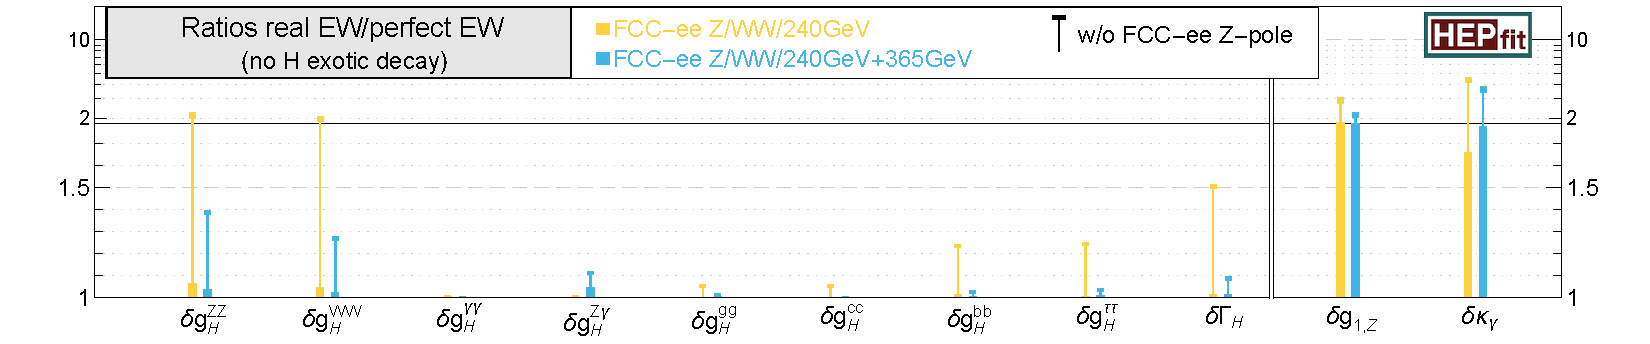
\includegraphics[width=\textwidth]{PhysicsCase/Figs/barplotsnow-PZratio-xo1-smpar-Ext_FSR.pdf}
\caption{Impact of \PZ-pole measurements on the Higgs coupling, Higgs decay width, and anomalous triple gauge-boson coupling ($\delta g_{1,\PZ}$ and $\delta \kappa_\gamma$) precision from the SMEFT fit interpretation. 
The ratio to the precision that would be obtained with infinitely precise \PZ-pole measurements is shown for fits 
that either exclude (`T' bars) or include (solid bars) the projected FCC-ee \PZ-pole run measurements, 
with the Higgs programme at 240\,GeV (yellow bars) and the additional data at 365\,GeV (blue bars). 
The colour code is the same as in Fig.~\ref{fig:Global_Fit}. Adapted from Ref.~\cite{deBlas:2022ofj}. 
}
\label{fig:ZpoleHiggsUnc}
\end{figure}

Not all the $6 \times 10^{12}$ \PZ bosons expected during the \PZ-pole run are needed 
to reach the precision on the $\PZ\Pe\Pe$ vertex required to fully mitigate the EW contamination in the Higgs couplings determination.
An estimate of the number of events needed to reduce such contamination to a level that does not hinder the Higgs couplings extraction 
is displayed in Fig.~\ref{fig:ZpoleHiggsUncVar}, 
which shows the deterioration in the precision of the most precise $\PH\PZ\PZ$ and $\PH\PQb\PQb$ couplings with respect to the full statistics of the FCC-ee \PZ-pole run, 
as a function of the number of events.
From the perspective of Higgs couplings, a few $10^9$ \PZ's, 
equivalent to less than a day of operation at the \PZ pole, 
are enough to saturate the Higgs coupling precision from the 240 and 365\,GeV runs.

\begin{figure}[ht]
\centering
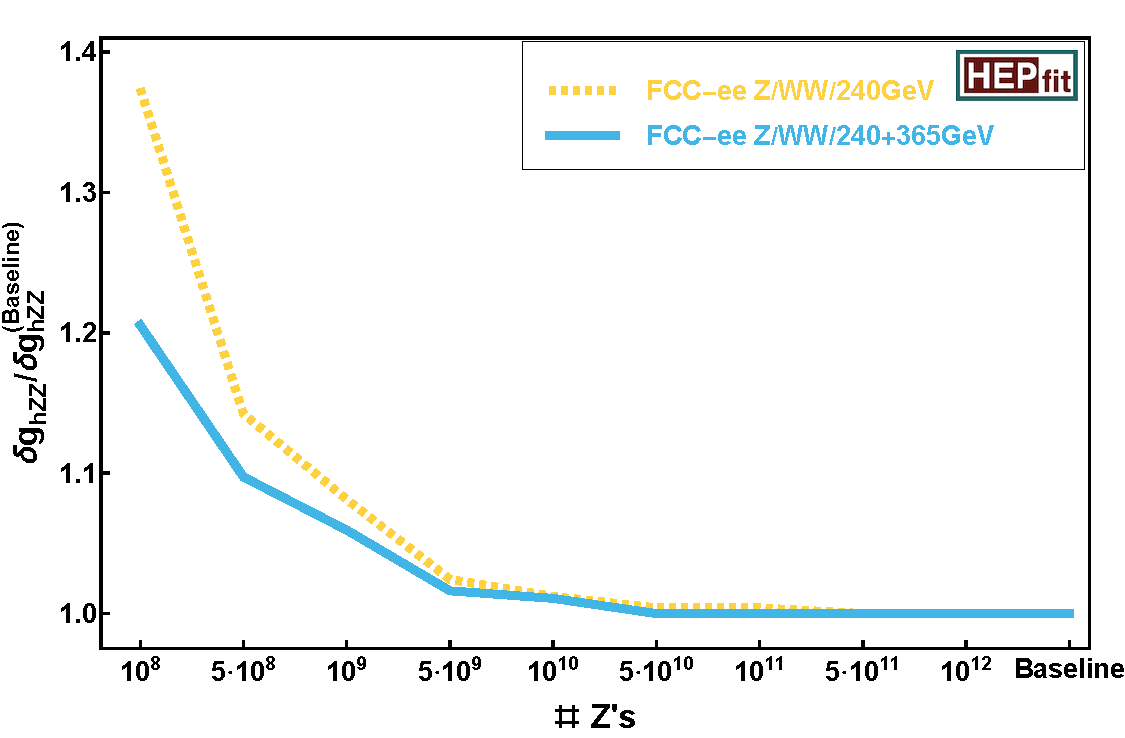
\includegraphics[width=0.48\textwidth]{PhysicsCase/Figs/barplotsnow_NZ_hZZ_newFSR.pdf}
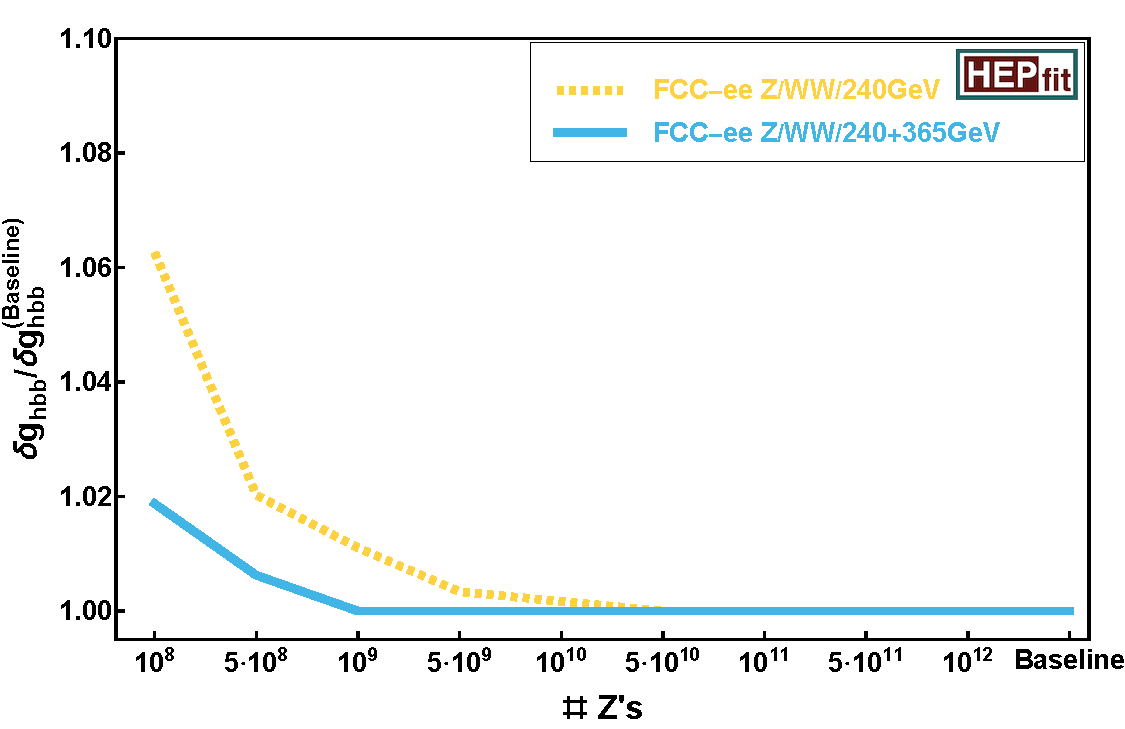
\includegraphics[width=0.48\textwidth]{PhysicsCase/Figs/barplotsnow_NZ_hbb_newFSR.pdf}
\caption{Estimated deterioration in the precision of the $\PH\PZ\PZ$ (left) and $\PH\PQb\PQb$ (right) couplings 
as a function of the number of \PZ's produced at FCC-ee,  
with respect to the baseline of $6\times 10^{12}$ events, 
for the FCC-ee programme up to 240\,GeV (yellow) and up to 365\,GeV (blue).}
\label{fig:ZpoleHiggsUncVar}
\end{figure}

\subsubsection{Impact of diboson measurements in Higgs couplings determination}

Together with gauge invariance, 
the assumption that electroweak symmetry is linearly realised in SMEFT implies a series of correlations 
between the new-physics effects on the electroweak properties of the SM particles, 
for example the aforementioned correlation between contributions to the $\PZ\Pe\Pe$ and $\PH\PZ\Pe\Pe$ interactions.
Another correlation relates modifications of the Higgs couplings to anomalous triple-gauge couplings (aTGCs): 
two out of the three aTGCs ($\delta g_{1,\PZ}$ and $\delta \kappa_\gamma$) are closely related to the Higgs couplings to vector bosons.

As shown in Ref.~\cite{Falkowski:2015jaa} for existing measurements and in Refs.~\cite{DeBlas:2019qco,deBlas:2022ofj} for FCC-ee projections, 
diboson and Higgs measurements are indeed sensitive to the same types of new-physics effects, 
so that diboson measurements can help constrain Higgs couplings (and vice-versa).
In the current SMEFT fits, all angular information available from the $\epem \to \PWp\PWm$ process is encoded in optimal observables, 
which bring a significant improvement~\cite{DeBlas:2019qco} with respect to the fits performed in the FCC CDR~\cite{fcc-phys-cdr,fcc-ee-cdr}, 
where only the (binned) \PW angular distribution was exploited to constrain the aTGCs. 
The inclusion of the full diboson kinematic information in the SMEFT fit also constrains all other possible interactions that can modify this process. 
The achieved relative precision on the Higgs couplings to gauge bosons and on the aTGCs is displayed in Fig.~\ref{fig:WWefficiency}, 
for three assumed values of the selection efficiency for the $\epem \to \PWp\PWm$ events: 
1\%, 45\% (default value in the following), and 100\%. 
A detailed experimental study of the projected precision is required to assess the ultimate sensitivity of the diboson measurements. 

\begin{figure}[ht]
\centering
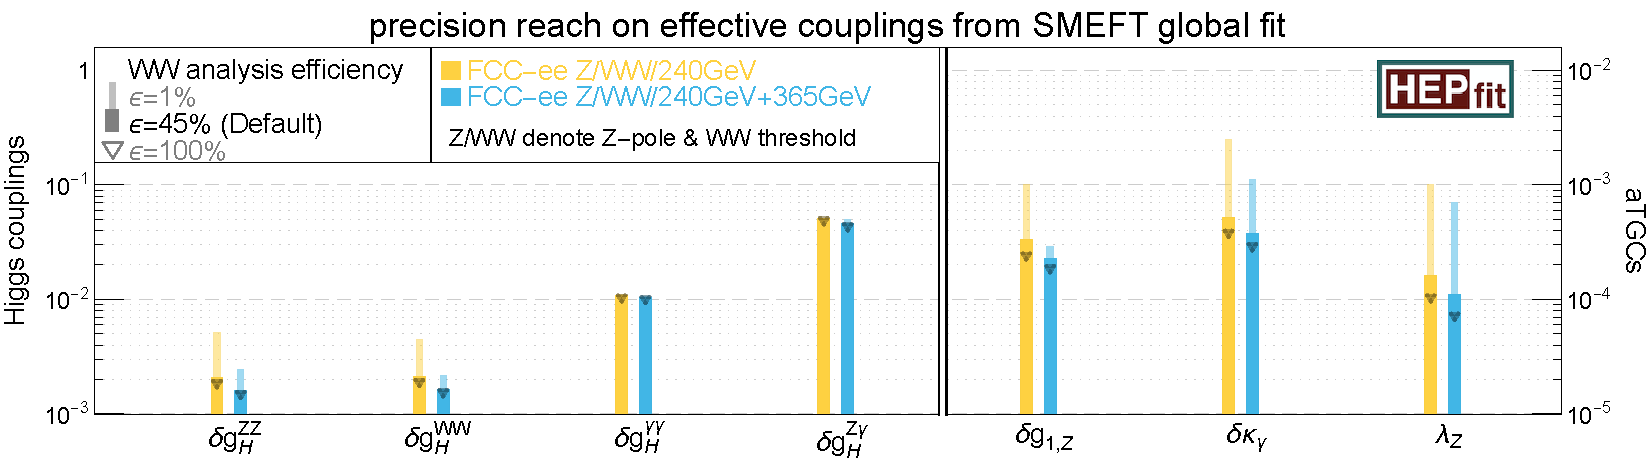
\includegraphics[width=\textwidth]{PhysicsCase/Figs/barplotsnow-xo1-100OO-smpar-upperpanel.pdf}
\caption{Relative precision of the determination of the Higgs couplings and aTGCs in the SMFET fit, 
as a function of the selection efficiency assumed in the $\epem \to \PWp\PWm$ study: 1\% (light shades), 45\% (solid bars, chosen as default value), and 100\% (triangles). The sensitivity comes mainly from the high-energy runs and the dependency at the $\PW\PW$ threshold remains small.
From Ref.~\cite{DeBlas:2019qco}.}
\label{fig:WWefficiency}
\end{figure}

\subsubsection{Complementarity between \texorpdfstring{\PZ}{Z}-pole and higher-energy runs}

Electroweak precision physics at the \PZ pole is typically thought to mainly constrain the $\hat{S}$ and $\hat{T}$ oblique parameters characterising the gauge 2-point functions, 
and not be as sensitive as higher energy runs for the $\hat{W}$ and $\hat{Y}$ parameters, 
the aTGCs, the Higgs self-energy and self-coupling, Higgs-vector-vector interactions, and a variety of four-fermion operators that, at tree-level, only enter off-pole observables~\cite{Barbieri:2004qk}. 
All these interactions, however, enter at higher-orders in the \PZ-pole observable theoretical predictions. 
The ultra-high precision provided by the \mbox{Tera-\PZ} event samples can overcome the extra loop-suppression factor of these operators 
and actually provide relevant constraints, competitive and complementary to higher-energy measurements 
where these interactions enter at leading order~\cite{Maura:2024zxz, Greljo:2024ytg}. 

This statement is illustrated in Fig.~\ref{fig:onpolevsoffpole}, 
which shows the sensitivity (in terms of effective scale of new physics $\Lambda$) to dimension-6 SMEFT operators entering in the four-fermion, 
gauge, and Higgs sectors, from the corresponding constraints in \PZ-pole observables on the one hand, 
and in higher-energy (denoted `above-pole') observables on the other. 
Besides often being better, the on-pole bounds also constrain different directions in the SMEFT space, 
as illustrated in Fig.~\ref{fig:onpoleoffpolecomplementarity} for two specific examples. 
As a consequence, the combination of on-pole and above-pole data very substantially reduces the overall volume of parameter space 
and, accordingly, tightens the constraints on specific models. 
The scope of the \mbox{Tera-\PZ} electroweak precision programme of FCC-ee is, therefore, 
far wider and more general than a na\"{\i}ve extrapolation of the already amazingly accurate SM confirmation from LEP data would suggest.

\begin{figure}[t]
\centering
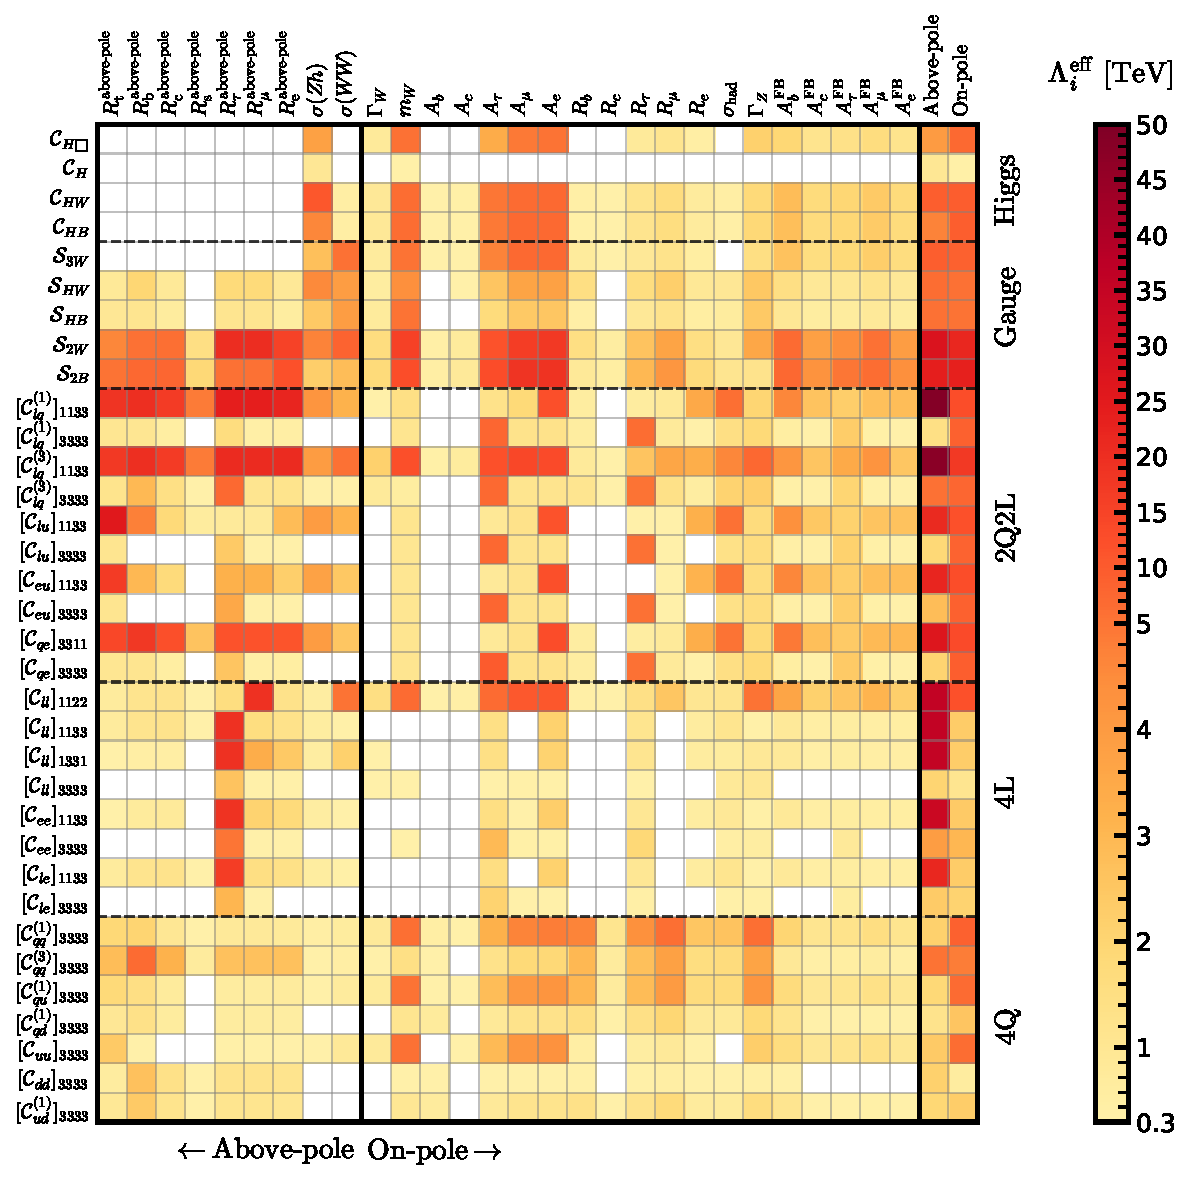
\includegraphics[width=\textwidth]{Physics/PhysicsCase/Figs/Coeff_Plot_Scale.pdf}
\caption{The 95\% CL projected sensitivities at FCC-ee to four-fermion, gauge, and Higgs dimension-6 operators, 
in terms of the effective scale of new physics $\Lambda$ (in TeV), 
from measurements of \PZ-pole observables (right part of the table) 
and of higher-energies observables (left part of the table).  
The rightmost two columns show the above- and on-pole combinations of all observables.
Adapted from Ref.~\cite{Maura:2024zxz}.}
\label{fig:onpolevsoffpole}
\end{figure}

\begin{figure}[ht]
\centering
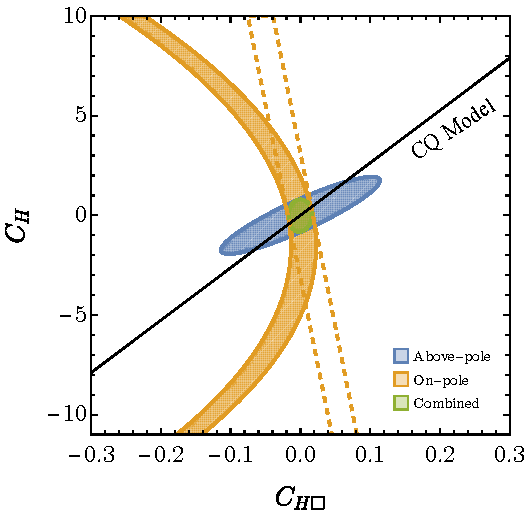
\includegraphics[width=0.46\textwidth]{Physics/PhysicsCase/Figs/CQmodelEFT.pdf}
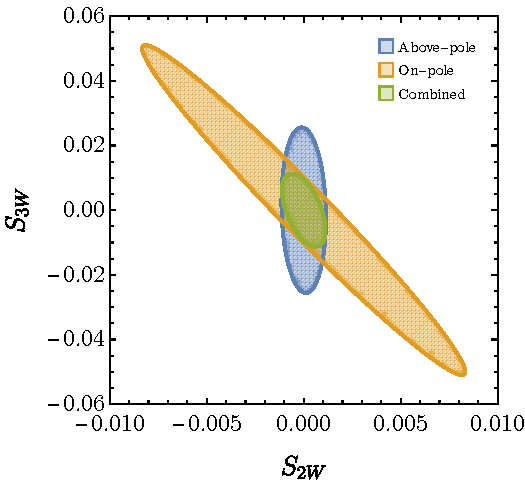
\includegraphics[width=0.49\textwidth]{Physics/PhysicsCase/Figs/3W_vs_2W.pdf}
\caption{Projected 68\% CL sensitivities at FCC-ee, from measurements at the \PZ pole (orange) and in higher-energy runs (blue), 
in the planes of Higgs self-energy vs.\ self-coupling (left) and of the $\hat{W}$ oblique parameter vs.\ an operator modifying anomalous triple-gauge couplings (right). 
The overall combined sensitivities (green) are much more constraining than the individual bounds. 
In the right plot, $S_{2W}$ and $S_{3W}$ are the coefficients of the dimension-6 operators 
$\mathcal{O}_{2W} = -1/2\, \left(D^\mu \, W_{\mu\nu}^I \right) \left(D_\rho \, W^{I\rho\nu}\right)$ and 
$\mathcal{O}_{3W} = \epsilon_{IJK} \, W_\mu^{I\nu} \, W_\nu^{J\rho} \, W_\rho^{K\mu}$,
both normalised with a scale of 1\,TeV. 
In the left plot, the region between the dashed orange lines corresponds to linearised on-pole constraints in the SMEFT operator coefficient
and the solid black line corresponds to a weak quadruplet scalar model. 
Adapted from Ref.~\cite{Maura:2024zxz}.}
\label{fig:onpoleoffpolecomplementarity}
\end{figure}

\subsubsection{Complementarity and synergy between FCC-ee and FCC-hh}

As shown in Table~\ref{tab:HiggsKappa3}, 
the precision of many Higgs boson couplings is expected to improve by about one order of magnitude with respect to the (partial and not assumption-free) knowledge 
that will be available at the end of the HL-LHC era. 
The precision of several couplings, such as $\PH\PGm\PGm$, $\PH\PQt\PQt$, $\PH\PGg\PGg$ or $\PH\PZ\PGg$, will however remain dominated by the HL-LHC knowledge,
even if they will only be made assumption-free by the FCC-ee absolute determination of the $\PH\PZ\PZ$ coupling. 
The few per-cent HL-LHC precision will be reduced by an order of magnitude at FCC-hh, by measuring ratios of branching ratios, 
free of systematic uncertainties and normalised by the FCC-ee precise coupling determination~\cite{fcc-phys-cdr}. 
The successive improvements of the Higgs boson coupling precision when going from HL-LHC to FCC-hh, 
benefitting on the way from the FCC-ee absolute and accurate coupling determination, are shown in Fig.~\ref{fig:hhimproveRare}.

\begin{figure}[ht]
\centering
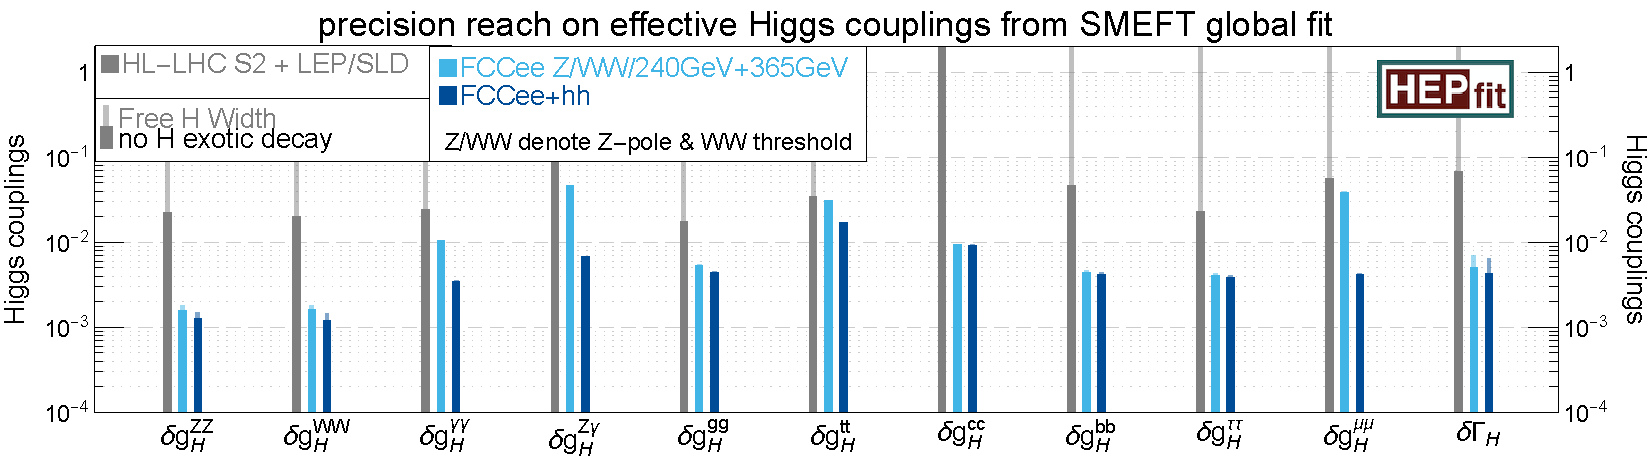
\includegraphics[width=\textwidth]{PhysicsCase/Figs/barplotsnow-h-sm-par-Htt_FSR.pdf}
\caption{Higgs coupling precision improvements with the global SMEFT fit from HL-LHC to FCC-hh, 
benefitting from the FCC-ee accurate and absolute coupling determination to optimally exploit the hadron collider measurements.
}
\label{fig:hhimproveRare}
\end{figure}

The FCC-ee role in the top Yukawa coupling determination is twofold. 
On the one hand, and as for all other Higgs couplings, 
the $\PH\PZ\PZ$ absolute determination at 240\,GeV enables a model-independent determination of the top Yukawa coupling from the HL-LHC data. 
On the other hand, the determination of the $\PZ\PQt\PAQt$ couplings from $\epem \to \PQt\PAQt$ at 365\,GeV~\cite{Janot:2015yza,defranchis_2024_cqd16-xhk71} 
can be used to normalise the measurement of the $\PQt\PAQt\PH$ cross section at FCC-hh to that of the $\PQt\PAQt\PZ$ cross section, 
and to reduce the uncertainty in the top Yukawa coupling down to the per-cent level~\cite{Mangano:2015aow}, as illustrated in the left panel of Fig.~\ref{fig:Interplay}. 

In this discussion, it is assumed that contributions from, e.g., dipole or four-fermion interactions in $\epem \to \PQt\PAQt$ or $\Pp\Pp \to \PQt\PAQt {\rm X}$ are negligible. 
The contributions of these four-fermion interactions to the $\PQt\PAQt\PH$ cross section at FCC-hh could be constrained from $\ttbar$ measurements. 
To constrain the contributions of the $\Pe\Pe\PQt\PQt$ four-fermion interactions to the $\epem \to \PQt\PAQt$ cross section, 
extra handles might need to be identified, during the next phase of the study, 
to lift the approximate flat directions that could appear in a global top-quark analysis.

\begin{figure}[t]
\centering
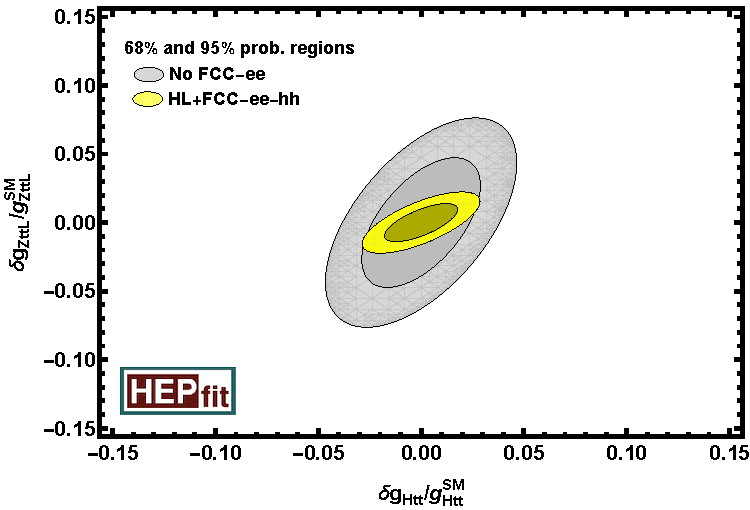
\includegraphics[width=0.49\textwidth]{PhysicsCase/Figs/ZttHttplot_FCCee.pdf}
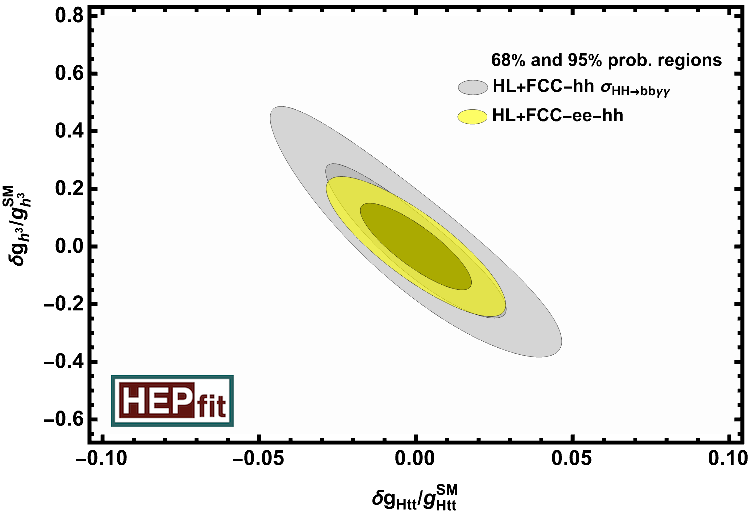
\includegraphics[width=0.49\textwidth]{Physics/PhysicsCase/Figs/H3Httplot_FCCee_noHL.pdf}
\caption{Results from ``toy'' fits to simulated data to illustrate the benefit of FCC-ee measurements 
in the FCC-hh determinations of the top Yukawa coupling (left) and of the Higgs self-coupling (right). 
In these fits, the total $\PH \PH \to \PQb\PAQb \PGg\PGg$ cross section is used as a proxy 
to discuss the interplay between the two couplings, following the parameterisation of Ref.~\cite{Azatov:2015oxa}. 
Simplifying assumptions are made on how the top EW couplings and the Higgs couplings to bosons and fermions are measured with a standalone FCC-hh.
The yellow (grey) areas show the 68\% and 95\% probability contours obtained assuming that the FCC-ee measurements are (are not) 
used in the coupling extraction from the FCC-hh data.}
\label{fig:Interplay}
\end{figure}

The Higgs boson self-coupling, $\kappa_\lambda$, will start being probed at HL-LHC, 
with an uncertainty that was estimated at the time of the 2020 ESPPU to be about 50\%, 
in a fit where only deformations of $\kappa_\lambda$ are allowed. 
Since then, improved analysis techniques and the inclusion of additional decay channels have reduced this uncertainty to 26\%~\cite{HLLHCProjections}.
The larger acceptance of the upgraded HL-LHC trackers is likely to bring it well below 25\%. 
In $\epem$ collisions, one-loop radiative corrections, that involve the Higgs self-coupling, to the Higgs boson production cross sections, 
are proportional to $\kappa_\lambda$. 
These corrections amount to several per-cent in the SM at 240\,GeV and strongly depend on the centre-of-mass energy~\cite{McCullough:2013rea}.
With this energy dependence, the sub-percent precision of the FCC-ee Higgs cross-section measurements at 240 and 365\,GeV 
suffice to disentangle the effect of new physics in the $\PH\PZ\PZ$ coupling and in $\kappa_\lambda$, 
and allows a stand-alone determination of $\kappa_\lambda$ with a precision of 28\%, as shown in the left panel of Fig.~\ref{fig:Hselfcoupling1}. 
Besides being quantitatively competitive with HL-LHC projections, 
this precision is also qualitatively distinct, as it is achieved within an SMEFT framework that accounts for a broad variety of potential new physics effects.

\begin{figure}[t]
\centering
\vskip -0.5cm
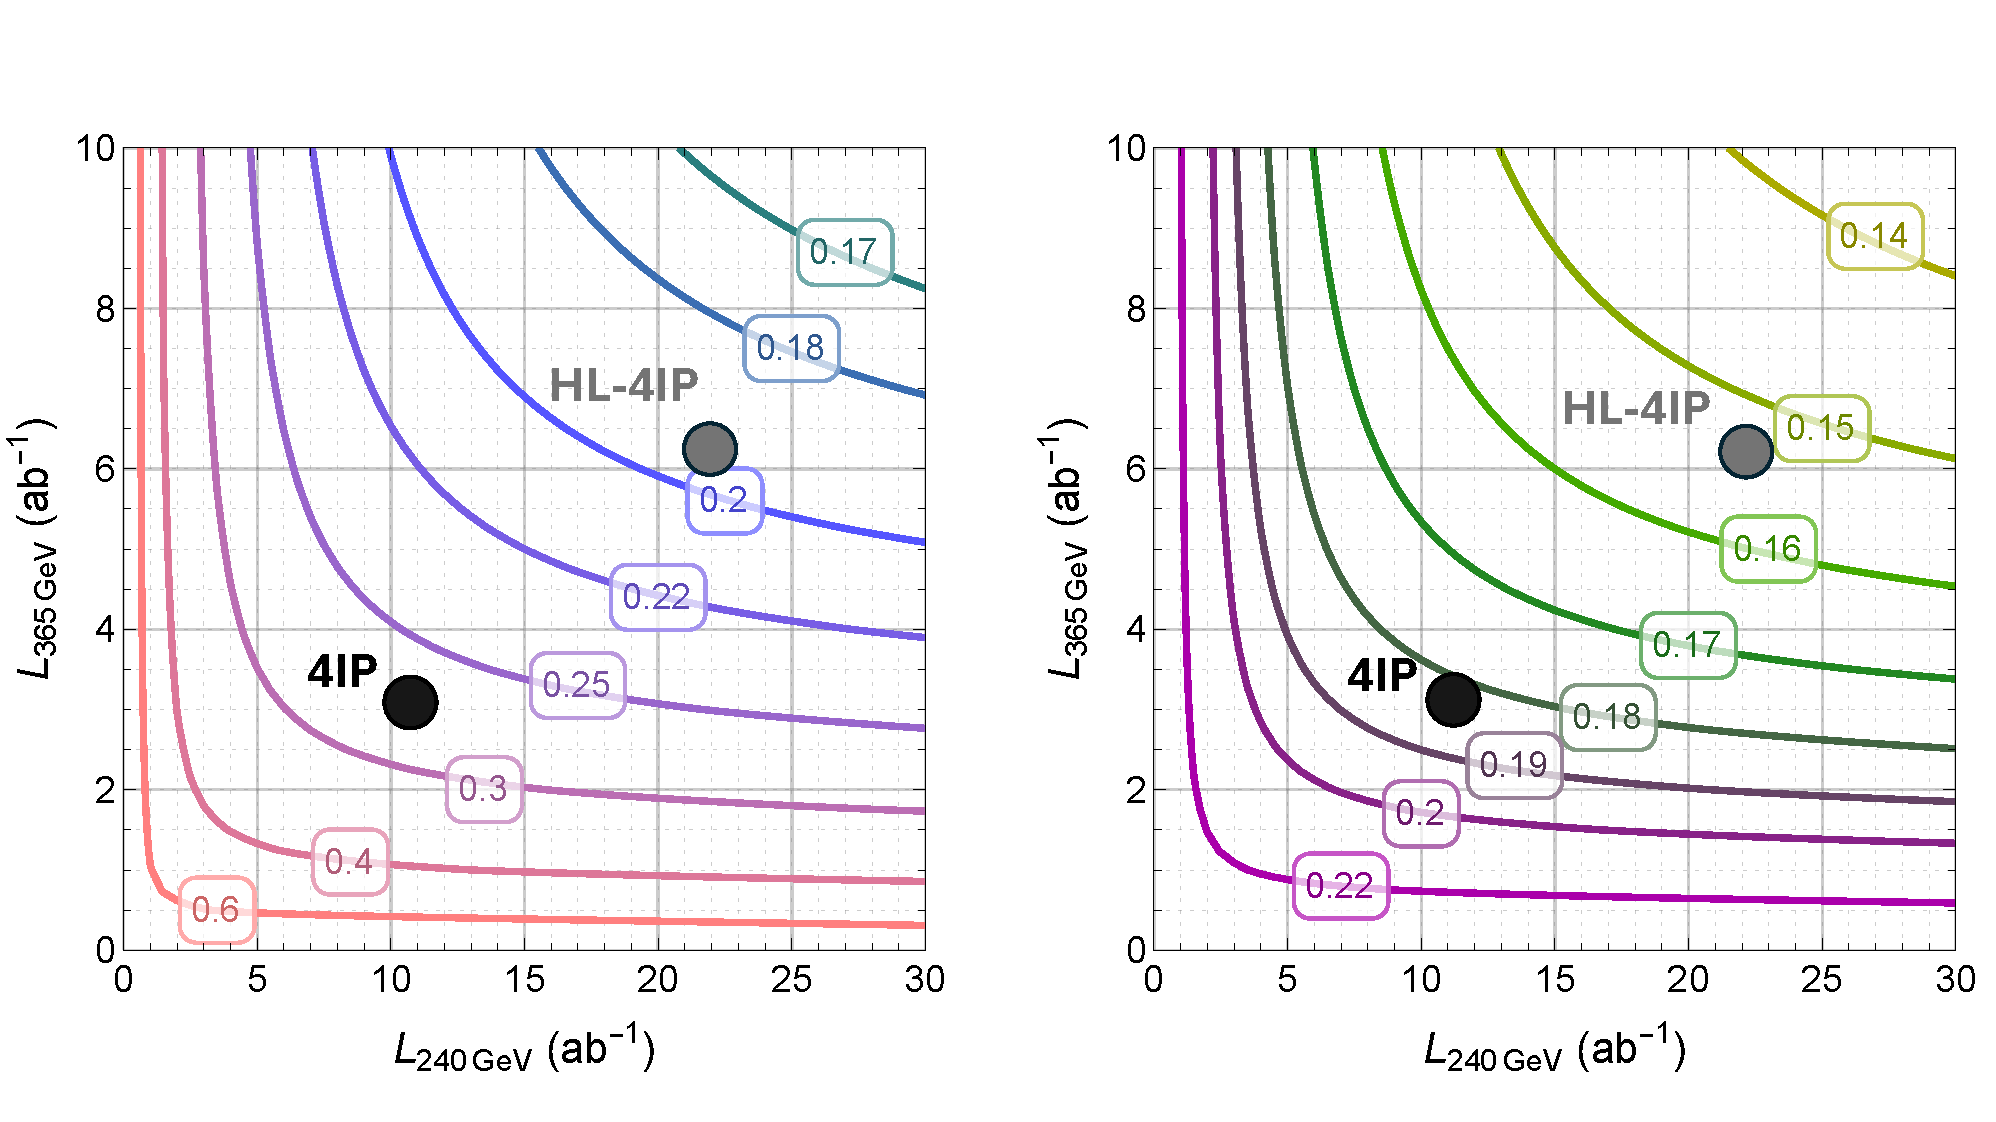
\includegraphics[width=0.9\textwidth]{Physics/PhysicsCase/Figs/Hselfcoupling-precision-1b.pdf}
\caption{The projected Higgs self-coupling relative precision from the SMEFT global fit, 
as a function of the integrated luminosities of the 240 and 365\,GeV runs, 
with FCC-ee alone (left) and FCC-ee combined with HL-LHC (right). 
The 4\,IP and HL-4\,IP dots represent the FCC-ee baseline scenario 
and an hypothetical scenario (described in the text) with doubled integrated luminosities at 240 and 365\,GeV, respectively.}
\label{fig:Hselfcoupling1}
\end{figure}

The combination of FCC-ee with HL-LHC therefore lifts the assumption made for the sole HL-LHC extraction, 
and significantly improves the overall precision on $\kappa_\lambda$ to 18\%, as shown in the right panel of Fig.~\ref{fig:Hselfcoupling1}.
If deemed important, it would be possible to double the FCC-ee integrated luminosity at 240 and 365\,GeV, 
and reach a precision close to 15\% on $\kappa_\lambda$, in a high-luminosity scenario dubbed HL-4\,IP in Fig.~\ref{fig:Hselfcoupling1}. 
The doubling of the integrated luminosity can be achieved either by running twice as long at these centre-of-mass energies, 
or by doubling the instantaneous luminosity, with a larger number of colliding bunches and/or a smaller vertical $\beta^\ast$ 
(along with a smaller vertical emittance), but without any hardware modifications to the collider, as explained in Ref.~\cite{frankAnnecy}. 

Recent studies~\cite{Asteriadis:2024xuk, Asteriadis:2024xts}
have shown that other new physics interactions, 
entering at the same order in perturbation theory, but absent from the SMEFT framework considered in this report, 
could marginally affect the $\kappa_\lambda$ extraction from single-Higgs processes.
In rare and extreme cases, the value of $\kappa_\lambda$ extracted from single production at FCC-ee data could differ from that with pair production at HL-LHC, 
a difference that would allow this new physics to be identified and constrained. 
More pragmatically, a global fit is needed to bound these other interactions and to mitigate their impact in the determination of $\kappa_\lambda$. 
The more operators are considered, the more observables are needed in the global fit. 
Some operators currently weakly bounded by experimental data, e.g., the four-fermion $\Pe\Pe\PQt\PQt$ operator, 
will require further investigation in the next phase of the study.

This subtlety is anecdotal in the grand vision of the FCC integrated project. 
Indeed, the Higgs self-coupling will be uniquely and unambiguously probed at FCC-hh via Higgs boson pair ($\PH\PH$) production. 
Current estimates, combining the $\PQb\PAQb \PGg\PGg$, $\PQb\PAQb \PGtp\PGtm$, $\PQb\PAQb\PZ\PZ$, and 4\,\PQb decay channels, 
suggest that a precise determination, with an uncertainty as small as 3.4\%, 
would be within the reach of a 100\,TeV $\Pp\Pp$ collider~\cite{Mangano:2020sao}, 
and probably better by a factor of two with progress similar to those made in the HL-LHC projections~\cite{HLLHCProjections} and in recent FCC-hh studies~\cite{Gallo:2024lin,mangano_2025_bzhc2-mem17}. 
The role of the different FCC stages in the determination of the Higgs self-coupling is summarised in Fig.~\ref{fig:Hselfcoupling2}.

\begin{figure}[ht]
\centering
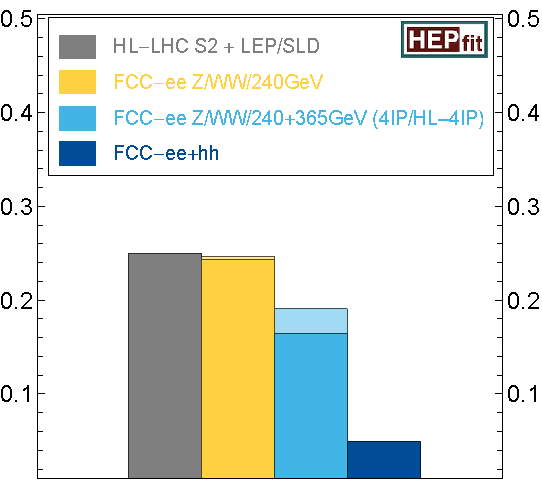
\includegraphics[width=0.4\textwidth]{Physics/PhysicsCase/Figs/barplot-h3i-sm-par-All.pdf}
\caption{Improvement in the determination of $\kappa_\lambda$ at FCC-ee 
(the darker colours are for the HL-4\,IP optimised scenario) 
and, subsequently, at FCC-hh. 
}
\label{fig:Hselfcoupling2}
\end{figure}

As for HL-LHC, this FCC-hh precision refers to an exclusive determination of the Higgs self-coupling, 
i.e., only considering deformations of $\kappa_\lambda$. 
Other new physics interactions, however, could modify the $\PH\PH$ production or decay rates and it is important to keep their uncertainties under control. 
While an inclusive analysis taking into account all these effects has not yet been undertaken, 
an illustration of the impact of such effects is displayed in the right panel of Fig.~\ref{fig:Interplay}. 
This figure shows how the uncertainty in the top Yukawa coupling modifies the $\kappa_\lambda$ precision 
from the measurement of the total $\Pg\Pg \to \PH\PH \to \PQb\PAQb \PGg\PGg$ cross section. 
The top Yukawa coupling enters with several powers in the different diagrams, contributing to $\sigma(\Pg\Pg \to \PH\PH)$. 
As noted above, the precise determination of the top Yukawa coupling at FCC-hh relies 
on the measurement of the $\sigma(\Pp\Pp \to \ttbar\PH)/\sigma(\Pp\Pp \to \ttbar\PZ)$ ratio, 
where the $\ttbar\PZ$ coupling itself should be allowed to vary within its experimental uncertainty, 
rather than being fixed to its assumed SM value. 
The plots in Fig.~\ref{fig:Interplay} show the impact of using, or not, the direct FCC-ee measurement of the $\ttbar\PZ$ coupling 
in the extraction of the top Yukawa coupling at FCC-hh (left panel) and the consequent impact on the $\kappa_\lambda$ determination (right panel). 

Finally, a concern was expressed 
about the sensitivity of the $\kappa_\lambda$ determination at HL-LHC if its true value were about twice the SM value ($\kappa_\lambda = 2$), 
for which the destructive interference between the box and triangle diagrams of the $\PH\PH$ production by gluon fusion in $\Pp\Pp$ collisions 
would significantly decrease the cross section. 
While the HL-LHC relative precision would actually not degrade for $\kappa_\lambda = 2$, the synergy with FCC-ee is, once more, remarkable here. 
Indeed, at FCC-ee the $\epem \to \PZ\PH$ production cross section is a linear function of the true value of $\kappa_\lambda$: 
$\sigma_{\PZ\PH} = \sigma_0 \times (1 + \alpha \, \kappa_\lambda)$, with $\alpha > 0$ (i.e., with a constructive interference). 
The FCC-ee relative precision on $\kappa_\lambda$, therefore, evolves as $1/\kappa_\lambda$ when the true value of $\kappa_\lambda$ increases. 
For $\kappa_\lambda = 2$, a stand-alone precision of 14\% would therefore be achieved at FCC-ee 
with an explicit EFT fit similar to that of Figs.~\ref{fig:Hselfcoupling1} and~\ref{fig:Hselfcoupling2}, 
improved to less than 10\% in the high-luminosity scenario.

\subsection{Discovery landscape}
\label{sec:PhysicsCaseBSM}

The discovery landscape for BSM physics at FCC-hh has been well documented in Ref.~\cite{Mangano:2017tke} 
and in the FCC CDR~\cite{fcc-phys-cdr}.  
Here, instead, the FCC-ee discovery landscape is discussed. 
While several results were already presented in the CDR, 
continuous work has taken place since, to refine or extend the scope of BSM searches, 
a notable example being the search for long-lived particles (LLPs) and heavy neutral leptons (HNLs).

\subsubsection{BSM exploration potential}

The capability and versatility of FCC-ee to explore open questions about the origins and nature of the Universe is immense. 
In addition to probing the known elementary particles and fundamental forces with the highest precision, 
it can survey uncharted territory both directly towards ultra-weak couplings and indirectly at very high energies, 
up to 100\,TeV, for so-far unknown particles and interactions. 

At the centre of many mysteries lies the Higgs boson. 
Besides enabling a much sharper picture of the Higgs boson and testing its (non-)SM nature, 
the $\PZ\PH$ run can also provide crucial model-independent sensitivity to its invisible decay mode(s), 
which probe the Higgs portal to dark sectors. 
Ultimately, an explanation for the origin of the Higgs mechanism itself is sought. 
From what underlying theory does the Higgs sector emerge? 
While this outstanding question is sufficient motivation in itself, 
a more fundamental description of the nature of electroweak symmetry breaking is, moreover, 
expected to be associated with new theoretical principles addressing the hierarchy problem, 
a naturalness strategy that has proven useful in the past 
and whose success or failure now would be of profound importance~\cite{Giudice:2008bi, Craig:2022uua}. 
These theories typically extend the symmetries of the SM, for example in supersymmetric, composite, 
or extra-dimensional frameworks~\cite{Fox:2022tzz}. 
More recent proposals involving light new physics include novel types of cosmological dynamics~\cite{Asadi:2022njl}. 
Alternatively, something radically new altogether may manifest in direct searches, 
indirectly by measuring higher-dimensional operator coefficients 
or spectacularly in unforeseen types of exotic signatures. 
It is crucial to fully explore the Higgs boson as much as possible above the TeV scale.

A deeper understanding of the scalar sector of the SM can also show 
whether the early Universe underwent a first-order electroweak phase transition (FOEWPT) or not, 
knowledge that is crucial for understanding the matter-antimatter asymmetry. 
As an example, in the real scalar singlet model, 
a FOEWPT is correlated with a modification of the Higgs coupling to \PZ bosons 
in a way that can be explored almost entirely by FCC-ee (Fig.~\ref{fig:realscalarsinglet}). 
Furthermore, a FOEWPT can also lead to gravitational wave (GW) signatures, 
which could be detectable by future GW observatories, such as LISA. 
Since it will be difficult to disentangle these signals from other astrophysical phenomena, 
precisely measuring the Higgs properties at colliders could have an important role to play 
in settling this important question~\cite{Friedrich:2022cak}. 
The synergy between cosmology and particle physics has been fruitful in the past 
and may well lead to a more profound understanding of the nature of the electroweak phase transition, 
exploring whether it had a role to play in the origin of matter.

\begin{figure}[t]
\centering
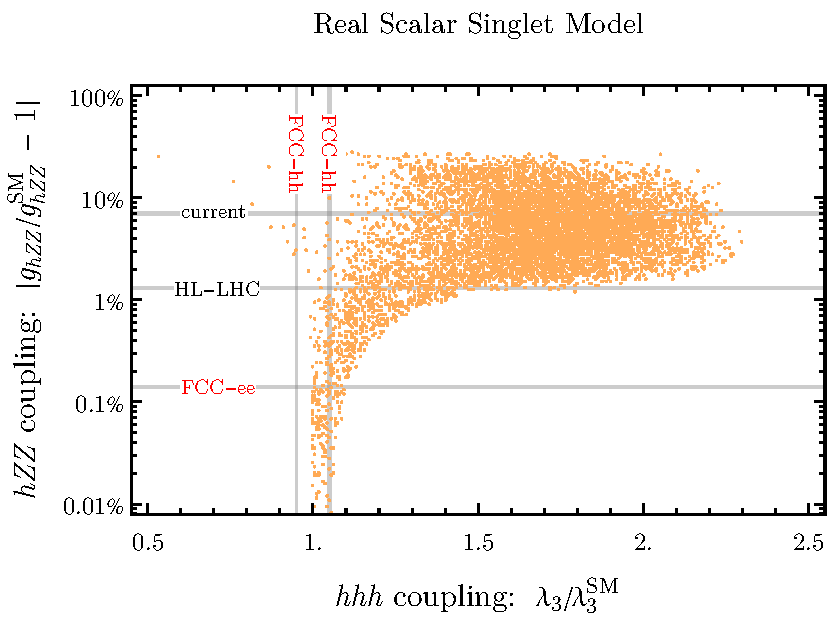
\includegraphics[width=0.7\linewidth]{PhysicsCase/Figs/realscalarsinglet_FSR.pdf}
\caption{Scan of the parameter space for a real scalar singlet model, 
where all points shown have a first-order electroweak phase transition, 
plotted in the plane of the fractional change in the Higgs coupling to a pair of \PZ bosons relative to its SM value (`hZZ coupling') 
vs.\ the triple-Higgs coupling normalised to its SM value (`hhh coupling').
The space outside the two FCC-hh lines and above the FCC-ee line can be covered at those facilities. 
Adapted from Ref.~\cite{Huang:2016cjm} and scaled to baseline luminosities.  
}
\label{fig:realscalarsinglet}
\end{figure}

The power of FCC-ee to probe the Higgs boson at much higher resolution than accessible today 
is that it enables peering further into the cloud of quantum fluctuations surrounding it. 
The envisioned precision indirectly opens a window onto physics at multi-TeV energies, 
around the level of current electroweak precision observables from LEP but uniquely sensitive to the Higgs boson. 
Given the number of possible BSM Feynman diagrams contributing virtually to these quantum fluctuations, 
there is a tremendous variety of possible new physics scenarios solving shortcomings of the SM that cannot be tested by other means. 
Similar to the past Fermi theory, the SMEFT is an EFT that maps out the path for continued exploration of what lies far beyond.  
For this essential programme of indirect BSM exploration through the SMEFT, FCC-ee is just indispensable. 

Non-decoupling particles  get most of their mass from the Higgs mechanism,  
requiring a more general EFT framework than SMEFT, known as HEFT, 
to accurately capture their low-energy phenomenology~\cite{Banta:2021dek}. 
Their coupling to the Higgs boson has a lower bound and unitarity requires their mass to have an upper limit. 
Their parameter space is therefore finite and can be comprehensively covered by FCC-ee, as detailed in Ref.~\cite{Crawford:2024nun}.
An interesting open question --- 
is the Higgs responsible for most of the mass of any other particles beyond the SM ones? ---
could then be basically settled. 

A further qualitative leap in resolving power comes from studying the \PZ boson at the \PZ-pole run of FCC-ee. 
A \mbox{Tera-\PZ} factory, with five orders of magnitude more \PZ bosons than at LEP, 
is another truly exciting prospect in its breadth of SM physics and spectacular BSM sensitivity. 
While the measurements at a Higgs factory bring the knowledge of the Higgs sector 
up to the high-precision standards of LEP electroweak precision observables, 
a new era of ultra-high precision observables will begin with \mbox{Tera-\PZ}. 
This ultra-high precision gives FCC-ee an indirect sensitivity to scales of several tens of TeV for weakly-coupled new physics, 
while the sensitivity for strongly coupled physics can reach 100\,TeV. 
To consolidate this sensitivity, the statistical precision reached by the very large \mbox{Tera-\PZ} event samples 
must be matched by a new generation of challenging theoretical calculations at higher electroweak loop orders, 
the development of which is another benefit of the FCC-ee physics programme: 
pushing the boundaries of experiment also expands the frontiers of theory and the understanding of quantum field theory.

After the \PZ boson, the \PW boson can also be used as a precision tool at FCC-ee. 
Its mass is one of the most precisely measured parameters that can be calculated in the SM and is thus of utmost importance. 
The production of almost $5 \times 10^8$ \PW bosons during the planned runs at the $\PW\PW$ threshold and above 
will provide tests of the SM and of a plethora of BSM models with a precision at least one order of magnitude better than today.
The combination of multi-\PZ and \PW production will measure the gauge-boson sector with the sharpest cutting-edge precision, 
leading not only to an unprecedented overview at the microscopic scale of electroweak physics 
but also offering sensitivity to a far broader range of physics intricately linked across the SM, 
and SMEFT more generally, by precision quantum effects.

Going to its highest energy, FCC-ee can explore physics associated with the heaviest known particle, the top quark, 
with the $\ttbar$ run. 
Its mass plays a fundamental role in the prediction of SM processes 
and for the cosmological fate of the metastable vacuum if the SM were extended up to $10^{10}$\,GeV 
or higher~\cite{Degrassi:2012ry,Buttazzo:2013uya,Bednyakov:2015sca,Andreassen:2017rzq}. 
An improvement by more than an order of magnitude, achievable at FCC-ee~\cite{defranchis_2024_cqd16-xhk71}, 
is necessary to perform the above-mentioned precision tests at the quantum level. 
This improvement goes hand in hand with significant progress in the experimental determination 
of the strong coupling constant~\cite{dEnterria:2022hzv}, one of nature's fundamental parameters. 
The large top quark mass suggests that it plays a unique role, 
not only in Higgs and flavour physics, but also in relation with new, so far unobserved, phenomena. 
Indeed, proposed solutions to important open questions motivate couplings of BSM physics to the third generation, 
which also happens to be among the least constrained sectors of the SM. 
Therefore, the precise measurements of the top quark mass and other top quark characteristics 
are crucial for BSM precision exploration.

As a heavy flavour factory, FCC-ee can also investigate the other crucial third generation particles, 
the tau lepton and the bottom quark. 
At the \PZ-pole run, a record number of `clean' \PB mesons and \PGt leptons are expected to be produced, 
the rare decays of which offer exceptional insight into flavourful processes beyond several tens of TeV in energy. 
Exploring the flavour structure of the SM in new regimes can yield clues as to its origin 
and potentially reveal BSM symmetries and selection rules. 
In addition to testing BSM flavour models, 
it provides a valuable experimental probe of CP violation and lepton flavour violation/universality 
that can arise generically in BSM extensions.

Finally, following the proposals and approvals at LHC of `parasite' detectors that enhance its physics potential, 
it is possible to also envision additional experiments at FCC at different locations~\cite{Wang:2019xvx,Tian:2022rsi, Lu:2024fxs}. 
Notably, the civil engineering provides FCC-ee with much bigger detector caverns (Chapter~\ref{sec:caverns}) 
than needed for a lepton collider, in order to use them later for FCC-hh. 
It would then be possible to, e.g., 
install instrumentation in the cavern walls to search for new long-lived particles~\cite{Chrzaszcz:2020emg}. 

Even in the absence of no-lose theorems for the discovery of BSM physics, whether in particle physics or anywhere else, 
the case for a general-purpose particle observatory to carry out fundamental science at the smallest accessible scales 
remains as strong as ever in the face of unanswered questions. 
The purpose of FCC-ee is to improve the knowledge of the Universe and explore its fundamental origins. 
On both these fronts, it is guaranteed to make significant progress.

\subsubsection{Tera-\texorpdfstring{\PZ}{Z} sensitivity to heavy new physics}

The extensive physics programme and unprecedented precision of FCC-ee 
renders it uniquely suited to a general exploration of the zeptoscale. 
In particular, the understanding of the role of the \mbox{Tera-\PZ} programme at FCC-ee 
in discovering evidence for BSM physics has evolved significantly in recent years.  
The picture that has emerged is that, if there is heavy new BSM physics coupled to the SM fields that modifies SM observables, 
\mbox{Tera-\PZ} is well placed to find traces of it.  
This reasoning has been developed in the context of concrete models concerned with the flavour puzzle~\cite{Allwicher:2023shc} 
and the microscopic origins of the Higgs boson~\cite{Stefanek:2024kds, Knapen:2024bxw}. 
Even if a broad and agnostic view of the motivation for the presence of new physics is taken, 
\mbox{Tera-\PZ} offers discovery potential for almost any scenario 
that leads to tree-level modifications of the SM~\cite{Allwicher:2024sso, Gargalionis:2024jaw}.

When considering the possibility of new physics at the TeV scale, 
it is incumbent upon any model-builder to account for all aspects relating to flavour.  
Since precision flavour observables have, for decades, 
provided a powerful indirect window onto physics at the shortest accessible distances, 
it is common that putative new physics scenarios fall foul of flavour constraints, 
requiring the mass scale of new states to greatly exceed the TeV scale.  
It is important, therefore, to identify and classify new physics scenarios 
that can be consistent with the present suite of experimental constraints.  
In Ref.~\cite{Allwicher:2023shc} it was reported that new physics with an approximate $\text{U}(2)^5$ flavour symmetry 
could exist at very low scales whilst remaining consistent with constraints. 
The high energy states in such a scenario necessarily give rise to modifications of the SM, 
with effects captured by families of dimension-6 SMEFT operators.  
The coefficients of these operators are shown in Fig.~\ref{fig:U(2)}, 
alongside present-day constraints from flavour, precision EW, and high-energy collider probes.   

\begin{figure}[ht]
\centering
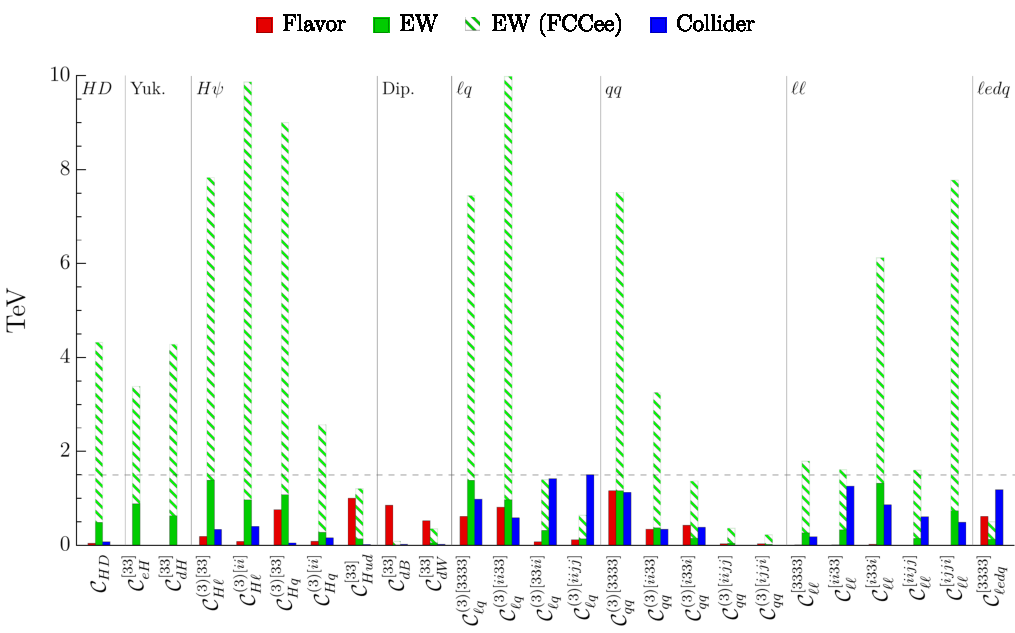
\includegraphics[width=0.75\linewidth]{PhysicsCase/Figs/plot5_2025_FSR.pdf}
\caption{The reach of FCC-ee precision electroweak observables (hatched) 
compared to present day flavour, electroweak, and high energy collider constraints, 
for all operators consistent with $\text{U}(2)^5$-symmetric flavour physics at the new physics matching scale. 
The bounds are 3\,$\sigma$ single-parameter fits, 
obtained running from a scale of 3\,TeV with full resummation of the logarithmic terms. 
Taken from Ref.~\cite{Allwicher:2023shc}. }
\label{fig:U(2)}
\end{figure}

It is clear that new physics states as low as the TeV scale are presently compatible with observations.  
On the other hand, projections from a precision EW programme at FCC-ee, driven primarily by the \mbox{Tera-\PZ} programme, 
are shown to probe significantly beyond this scale, as far as 10\,TeV. 
Not only is the sensitivity of operators that enter electroweak precision at tree level enhanced to the tens of TeV scale, 
there are also many more third generation operators being constrained at loop level through RGE evolution. 
This observation would significantly impact the understanding of the new physics landscape at high energies 
and its interplay with flavour, providing opportunities to discover the effects of heavy new physics.

The previous discussion concerns the flavour structure of new physics scenarios.  
In contrast, Ref.~\cite{Stefanek:2024kds} focuses specifically on the question of Higgs compositeness.  
Composite Higgs models are a class of scenarios in which the Higgs boson is a composite bound state 
of a new strongly-coupled dynamics at the TeV scale and a potential precursor of extra spatial dimensions. 
These models offer compelling answers to the question of the microscopic origins of the Higgs sector of the SM, 
in analogy with the way in which QCD explains the existence and properties of the pions.  
However, a significant challenge to such a scenario follows from the magnitude of the Higgs boson Yukawa coupling to the top quark.  
This large coupling is difficult to accommodate in the most basic realisations, 
but it can arise if the left and/or right-handed top quarks are also partially composite.  
This observation thus brings flavour considerations to the fore when attempting to understand the origins of the Higgs sector.

Reference~\cite{Stefanek:2024kds} considers the role that an FCC-ee precision EW programme 
would play in probing the possibility of partial top quark compositeness. 
A custodial symmetry is typically assumed of such models to evade current electroweak precision bounds from the $T$ parameter, 
equivalent to a custodially-violating dimension-6 operator. 
However, the SM violation of custodial symmetry itself leads to a next-to-leading-log RG running into the $T$ parameter 
that can no longer be so easily evaded at FCC-ee. 
This renders large swathes of parameter space accessible to FCC-ee, as shown in Fig.~\ref{fig:Stefanek}, 
where FCC-ee projections are compared to nearer-term HL-LHC and flavour projections. 
A huge increase in projected reach is observed, to compositeness scales of at least 25\,TeV. 

\begin{figure}[ht]
\centering

\includegraphics[width=0.325\linewidth]{PhysicsCase/Figs/leftCompSummary.pdf}    

\includegraphics[width=0.325\linewidth]{PhysicsCase/Figs/mixedCompSummary.pdf}    

\includegraphics[width=0.325\linewidth]{PhysicsCase/Figs/rightCompSummary.pdf}
\caption{The FCC-ee reach for probing Higgs and top compositeness through the precision EW programme, 
as compared to nearer-term HL-LHC and flavour measurements.  
Taken from Ref.~\cite{Stefanek:2024kds}.  
Left, mixed, and right top partial compositeness are considered (left to right panels).}
\label{fig:Stefanek}
\end{figure}

A final consideration, developed in Refs.~\cite{Allwicher:2024sso, Gargalionis:2024jaw}, 
could be considered an `informed agnostic' perspective on the nature of heavy new physics.  
The leading low energy effects of any heavy new physics scenarios with states whose mass does not depend significantly on the Higgs field 
can be captured in the dim-6 operators of the SMEFT.  
However, that does not conversely mean that any pattern of dim-6 SMEFT operators 
corresponds to a legitimate heavy new physics scenario.  
Thus, it is too simplistic to perform EFT fits in the context of future colliders without paying heed to concrete UV scenarios.

\begin{table}[ht]
\centering
\caption{Heavy scalars, fermions, and vectors that can contribute to SMEFT at dimension-6 
with corresponding representations under $\text{SU}(3)_C \times \text{SU}(2)_L \times \text{U}(1)_Y$.  
Taken from Ref.~\cite{deBlas:2017xtg}.}
\label{tab:Granadadict}
    {\small
      \begin{tabular}{l|cccccccc}
        Scalar &
        ${\cal S}$ &
        ${\cal S}_1$ &
        ${\cal S}_2$ &
        $\varphi$ &
        $\Xi$ &
        $\Xi_1$ &
        $\Theta_1$ &
        $\Theta_3$ \\
         &
        $\left(1,1\right)_0$ &
        $\left(1,1\right)_1$ &
        $\left(1,1\right)_2$ &
        $\left(1,2\right)_{\frac 12}$ &
        $\left(1,3\right)_0$ &
        $\left(1,3\right)_1$ &
        $\left(1,4\right)_{\frac 12}$ &
        $\left(1,4\right)_{\frac 32}$ \\[1.3mm]
        %
        %
        &&&&&&&\\[-0.4cm]
        %
        %
         &
        ${\omega}_{1}$ &
        ${\omega}_{2}$ &
        ${\omega}_{4}$ &
        $\Pi_1$ &
        $\Pi_7$ &
        $\zeta$ &
        & \\ 
         &
        $\left(3,1\right)_{-\frac 13}$ &
        $\left(3,1\right)_{\frac 23}$ &
        $\left(3,1\right)_{-\frac 43}$ &
        $\left(3,2\right)_{\frac 16}$ &
        $\left(3,2\right)_{\frac 76}$ &
        $\left(3,3\right)_{-\frac 13}$ \\[1.3mm]
        % 
        %
        &&&&&&&\\[-0.4cm]
        %
        % 
         &
        $\Omega_{1}$ &
        $\Omega_{2}$ &
        $\Omega_{4}$ &
        $\Upsilon$ &
        $\Phi$ &
        &
        & \\
         &
        $\left(6,1\right)_{\frac 13}$ &
        $\left(6,1\right)_{-\frac 23}$ &
        $\left(6,1\right)_{\frac 43}$ &
        $\left(6,3\right)_{\frac 13}$ &
        $\left(8,2\right)_{\frac 12}$ \\[1.3mm]
        % 
\hline
Fermion &
        $N$ & $E$ & $\Delta_1$ & $\Delta_3$ & $\Sigma$ & $\Sigma_1$ & & \\
         &
        $\left(1, 1\right)_0$ &
        $\left(1, 1\right)_{-1}$ &
        $\left(1, 2\right)_{-\frac{1}{2}}$ &
        $\left(1, 2\right)_{-\frac{3}{2}}$ &
        $\left(1, 3\right)_0$ &
        $\left(1, 3\right)_{-1}$ & & \\[1.3mm]
        %
        &&&&&&&\\[-0.4cm]
        %
         &
        $U$ & $D$ & $Q_1$ & $Q_5$ & $Q_7$ & $T_1$ & $T_2$ \\
         &
        $\left(3, 1\right)_{\frac{2}{3}}$ &
        $\left(3, 1\right)_{-\frac{1}{3}}$ &
        $\left(3, 2\right)_{\frac{1}{6}}$ &
        $\left(3, 2\right)_{-\frac{5}{6}}$ &
        $\left(3, 2\right)_{\frac{7}{6}}$ &
        $\left(3, 3\right)_{-\frac{1}{3}}$ &
        $\left(3, 3\right)_{\frac{2}{3}}$ & \\[1.3mm]
%
\hline
        Vector &
        ${\cal B}$ &
        ${\cal B}_1$ &
        ${\cal W}$ &
        ${\cal W}_1$ &
        ${\cal G}$ &
        ${\cal G}_1$ &
        ${\cal H}$ &
        ${\cal L}_1$ \\
         &
        $\left(1,1\right)_0$ &
        $\left(1,1\right)_1$ &
        $\left(1,3\right)_0$ &
        $\left(1,3\right)_1$ &
        $\left(8,1\right)_0$ &
        $\left(8,1\right)_1$ &
        $\left(8,3\right)_{0}$ &
        $\left(1,2\right)_{\frac 12}$ \\[1.3mm]
        % 
        %
        &&&&&&&\\[-0.4cm]
        %
        % 
         &
        ${\cal L}_3$ &
        ${\cal U}_2$ &
        ${\cal U}_5$ &
        ${\cal Q}_1$ &
        ${\cal Q}_5$ &
        ${\cal X}$ &
        ${\cal Y}_1$ &
        ${\cal Y}_5$ \\
         &
        $\left(1,2\right)_{-\frac 32}$ &
        $\left(3,1\right)_{\frac 23}$ &
        $\left(3,1\right)_{\frac 53}$ &
        $\left(3,2\right)_{\frac 16}$ &
        $\left(3,2\right)_{-\frac 56}$ &
        $\left(3,3\right)_{\frac 23}$ &
        $\left(\bar 6,2\right)_{\frac 16}$ &
        $\left(\bar 6,2\right)_{-\frac 56}$ \\[1.3mm]
        % 
        %
      \end{tabular}
    }
\end{table}

\begin{figure}[ht]
\centering
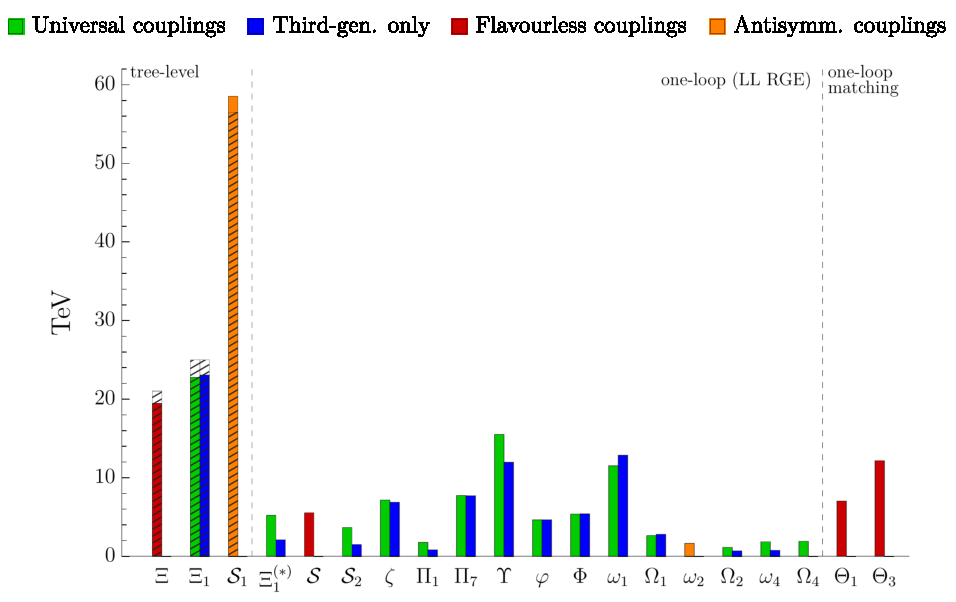
\includegraphics[width=0.65\linewidth]{PhysicsCase/Figs/newscalars_FSR.pdf}
\caption{Projected bounds on the masses of new scalar fields (the bounds are 2\,$\sigma$ fits, 
obtained running with the leading-logarithmic terms from a scale of 2\,TeV, 
at which the couplings to the SM particles are assumed to be unity, down to the mass of the \PZ).
`Flavourless couplings' correspond to models in which couplings of the new states to fermions are absent, 
`Universal couplings' correspond to equal couplings to all generations, and 
`Third-gen only' to new physics coupled only to the third generation fermions. 
The vertical dashed lines separate fields that contribute to EWPOs at tree level (left), 
via one-loop RG evolution (middle), and via one-loop matching (right). 
From Ref.~\cite{Allwicher:2024sso}, scaled to baseline luminosities.}
\label{fig:scalars6}
\end{figure}

As an informed middle ground, 
Refs.~\cite{Allwicher:2024sso, Gargalionis:2024jaw} considered all possible new physics scenarios 
where any dim-6 SMEFT operators are generated at tree-level.  
The number of possibilities is large, but finite, as detailed in Table~\ref{tab:Granadadict}.  
If any such scenario exists and modifies SM properties in any sector of the SM at dim-6, 
the precision EW programme at FCC-ee has sensitivity, 
as shown in Figs.~\ref{fig:scalars6}, \ref{fig:fermions6}, and~\ref{fig:vectors6}. 

As a matter of fact, FCC-ee can effectively probe virtually all heavy particles linearly coupled to the SM, 
with a sensitivity that reaches up to 100\,TeV at tree-level 
and $\mathcal{O}$(1--10)\,TeV at the one-loop level for $\mathcal{O}(1)$ couplings. 
This reach could extend even higher in the case of strongly-coupled new physics. 
Quantum RG effects are crucial.  
Any treatment that considers the SMEFT contributions of these states only at tree-level 
would overlook the majority of the sensitivity of the FCC-ee \mbox{Tera-\PZ} programme to their existence.

\begin{figure}[t]
\centering
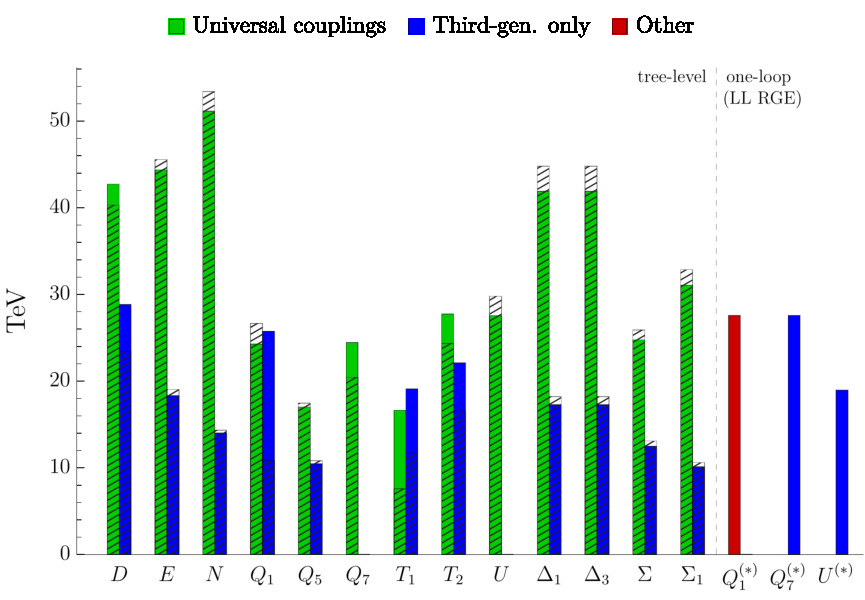
\includegraphics[width=0.65\linewidth]{PhysicsCase/Figs/newfermions_FSR.pdf}
\caption{Projected bounds on the masses of new vector fields. Same as for Fig.~\ref{fig:scalars6}.
}
\label{fig:fermions6}
\end{figure}

\begin{figure}[t]
\centering
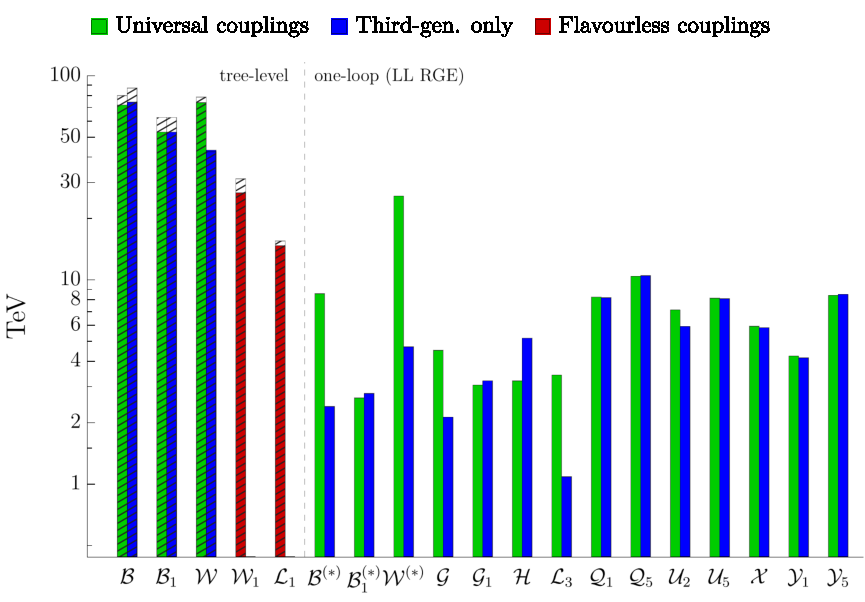
\includegraphics[width=0.65\linewidth]{PhysicsCase/Figs/newvectorslog_FSR.pdf}
\caption{Projected bounds on the masses of new fermion fields. Same as for Fig.~\ref{fig:scalars6}.
}
\label{fig:vectors6}
\end{figure}

Reference~\cite{Allwicher:2024sso} only considers the \mbox{Tera-\PZ} and $\PW\PW$ runs. 
Recently, the SMEFit Collaboration studied the impact of the various runs combined and individually. 
Details can be found in Refs.~\cite{terHoeve:2023pvs,Celada:2024mcf,smefit:2025}, 
including the slightly different EW-input scheme, 
which leads to some minor differences with respect to the results of Ref.~\cite{Allwicher:2024sso} for some models.  
Figure~\ref{fig:SMEFITmatched} demonstrates the exploratory power of the various runs 
to a variety of models in which the full one-loop matching is performed at the matching scale.  
Figures~\ref{fig:SMEFITscalars}, \ref{fig:SMEFITfermions}, and~\ref{fig:SMEFITvectors} 
consider selected scalar, fermion, and vector scenarios with RG-evolved Wilson coefficients 
but not one-loop matching, as in Figs.~\ref{fig:scalars6}, \ref{fig:fermions6}, and~\ref{fig:vectors6}.

\begin{figure}[ht]
\centering
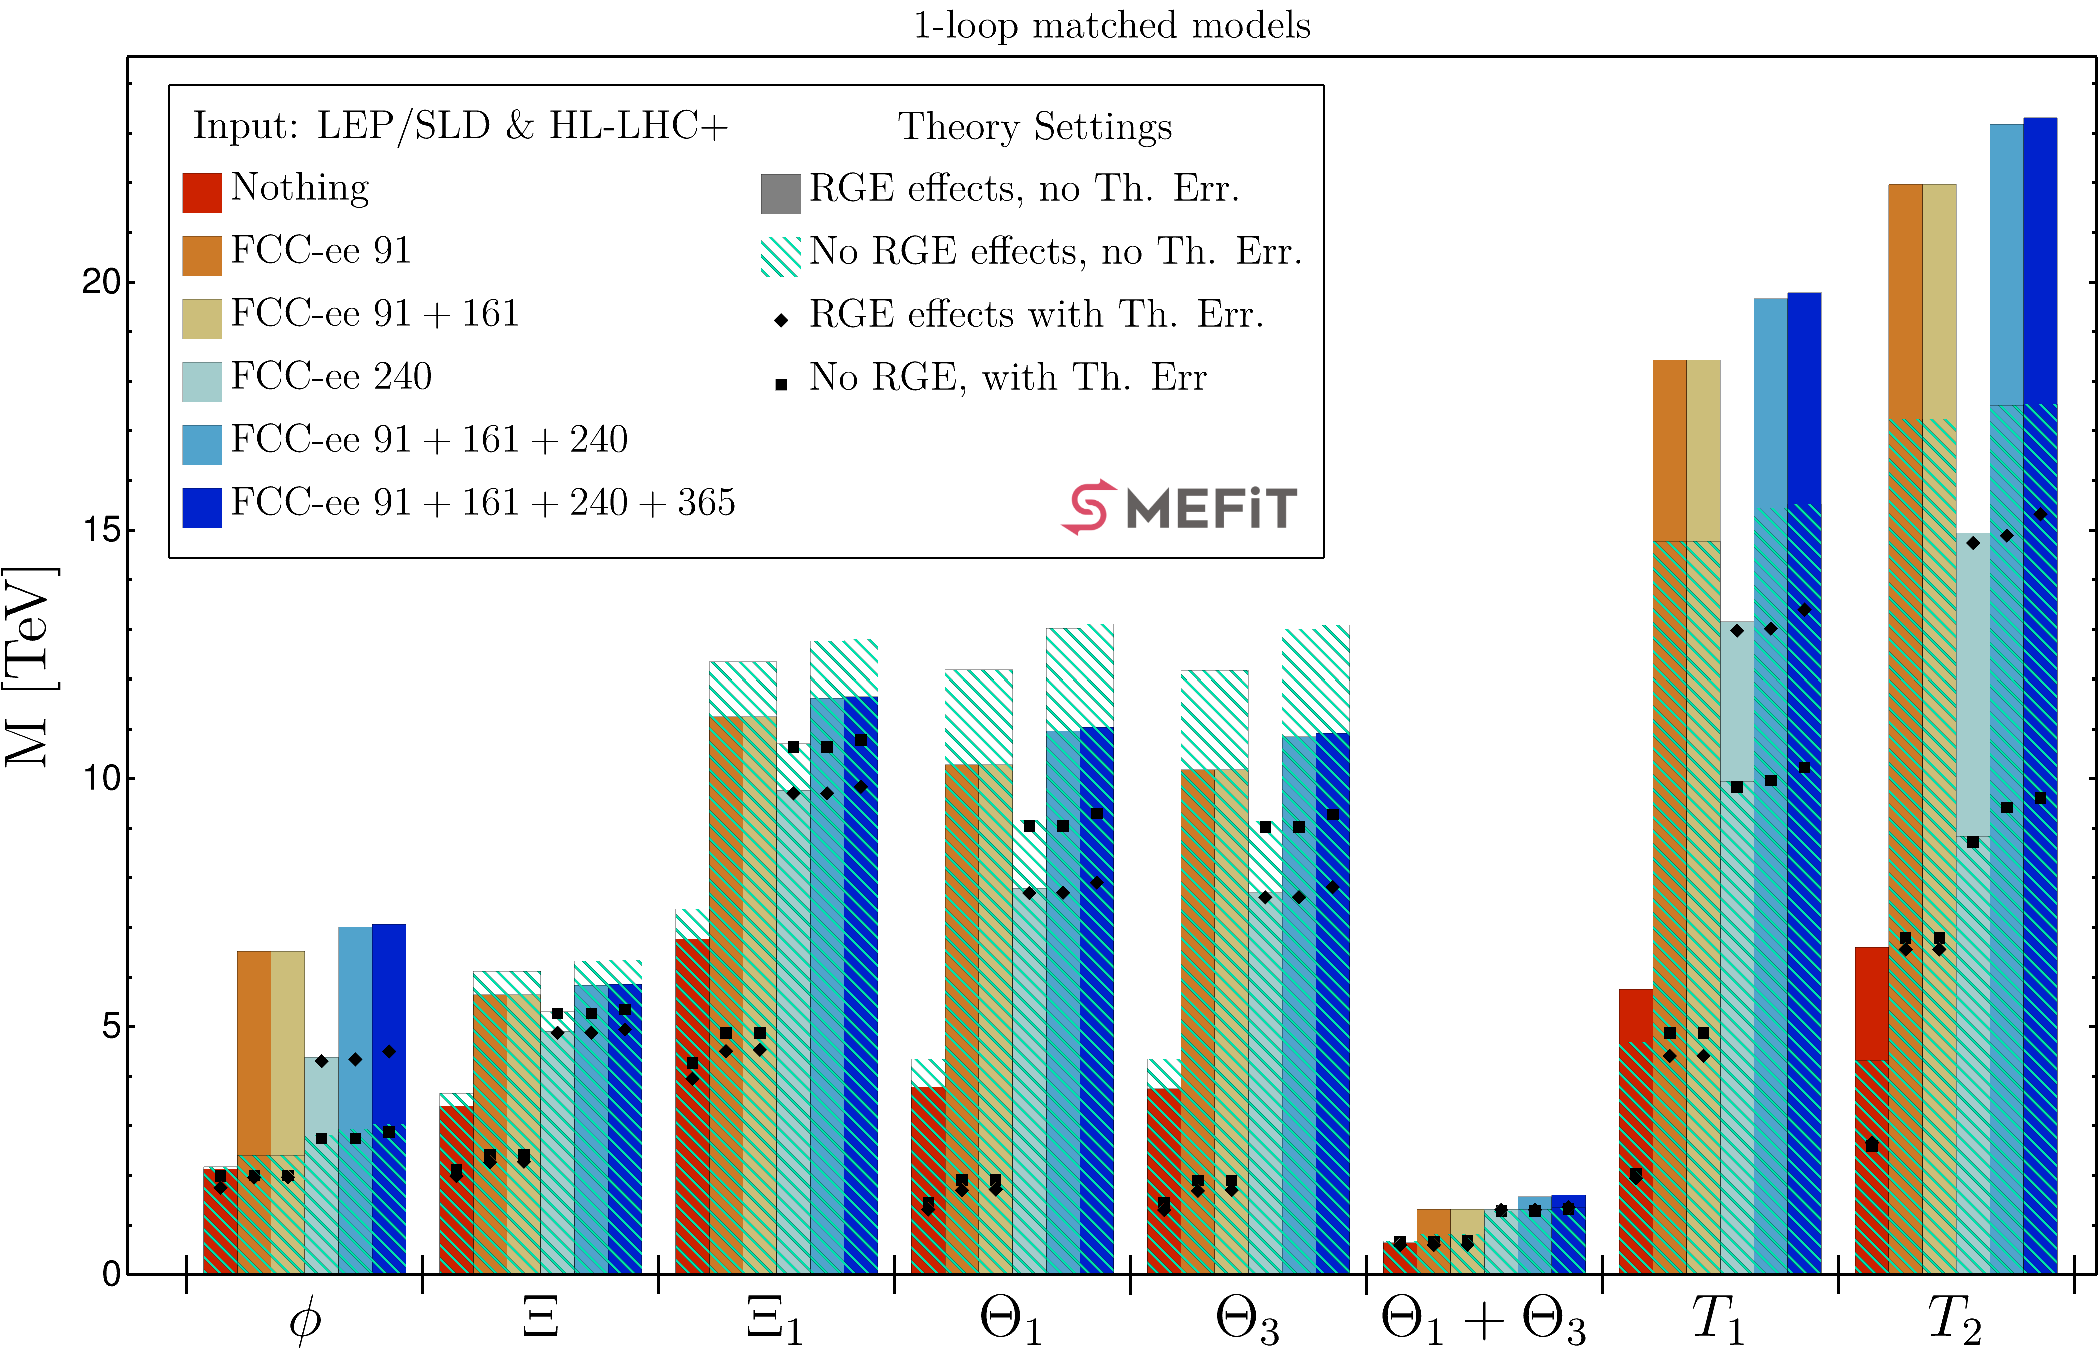
\includegraphics[width=0.65\linewidth]{PhysicsCase/Figs/plot_FCCFeasRep_runs_RGE_mass_UV_1LoopMatched_FSR.pdf}
\caption{Sensitivity (95\% CL) to a selection of models from Table~\ref{tab:Granadadict} 
with Wilson coefficients fully matched at one-loop 
(the bounds are obtained from a $\chi^2$ fit and the couplings of the new particle are set to unity at the matching scale, 
taken to be the mass of this heavy particle, 
the different operators are then run down to the \PZ boson mass with full numerical resummation of the logarithmic terms).   
In the case of new physics coupled to SM fermions, 
heavy scalar and fermions couple to the third generation only, 
while vectors couple to third-generation quarks and all generations of leptons.  
The starting scenario corresponds to all LEP/SLD and LHC constraints anticipated by the end of HL-LHC operation.
Additional combinations of FCC-ee runs are then shown. 
Black markers denote anticipated constraints were the theory uncertainties to remain as at present.  
The $\Theta_1+\Theta_3$ model corresponds to the custodial quadruplet model of Refs.~\cite{Logan:2015xpa,Chala:2018ari,Durieux:2022hbu}.}
\label{fig:SMEFITmatched}
\end{figure}
\begin{figure}[ht]
\centering
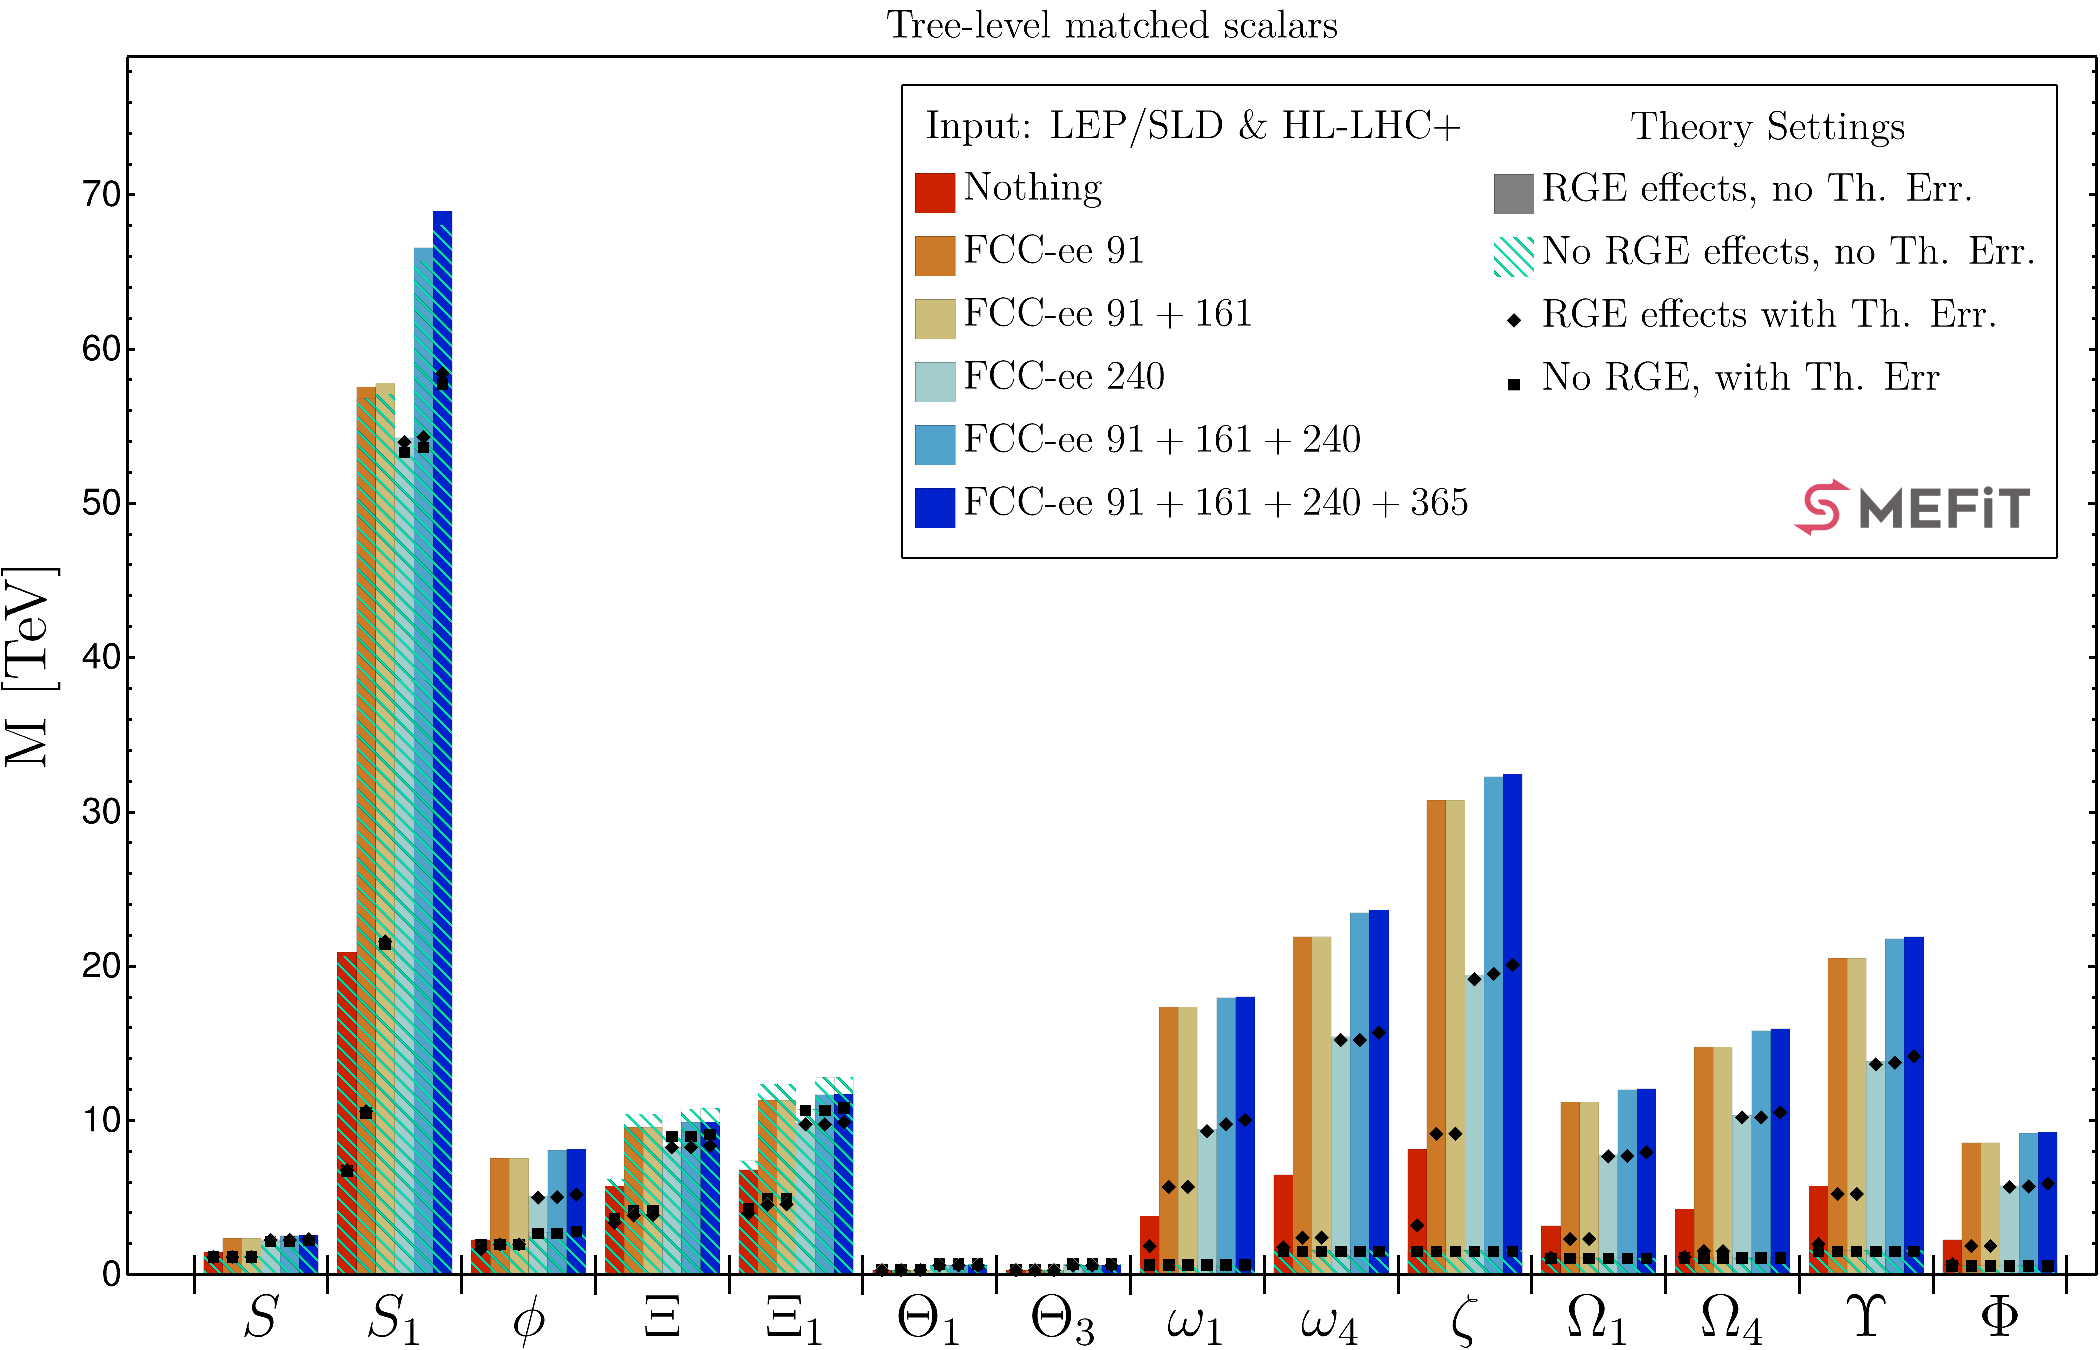
\includegraphics[width=0.65\linewidth]{PhysicsCase/Figs/plot_FCCFeasRep_runs_RGE_mass_UV_Scalars_FSR.pdf}
\caption{As Fig.~\ref{fig:SMEFITmatched}, but without the one-loop matched terms, for scalars.}
\label{fig:SMEFITscalars}
\end{figure}

\begin{figure}[ht]
\centering
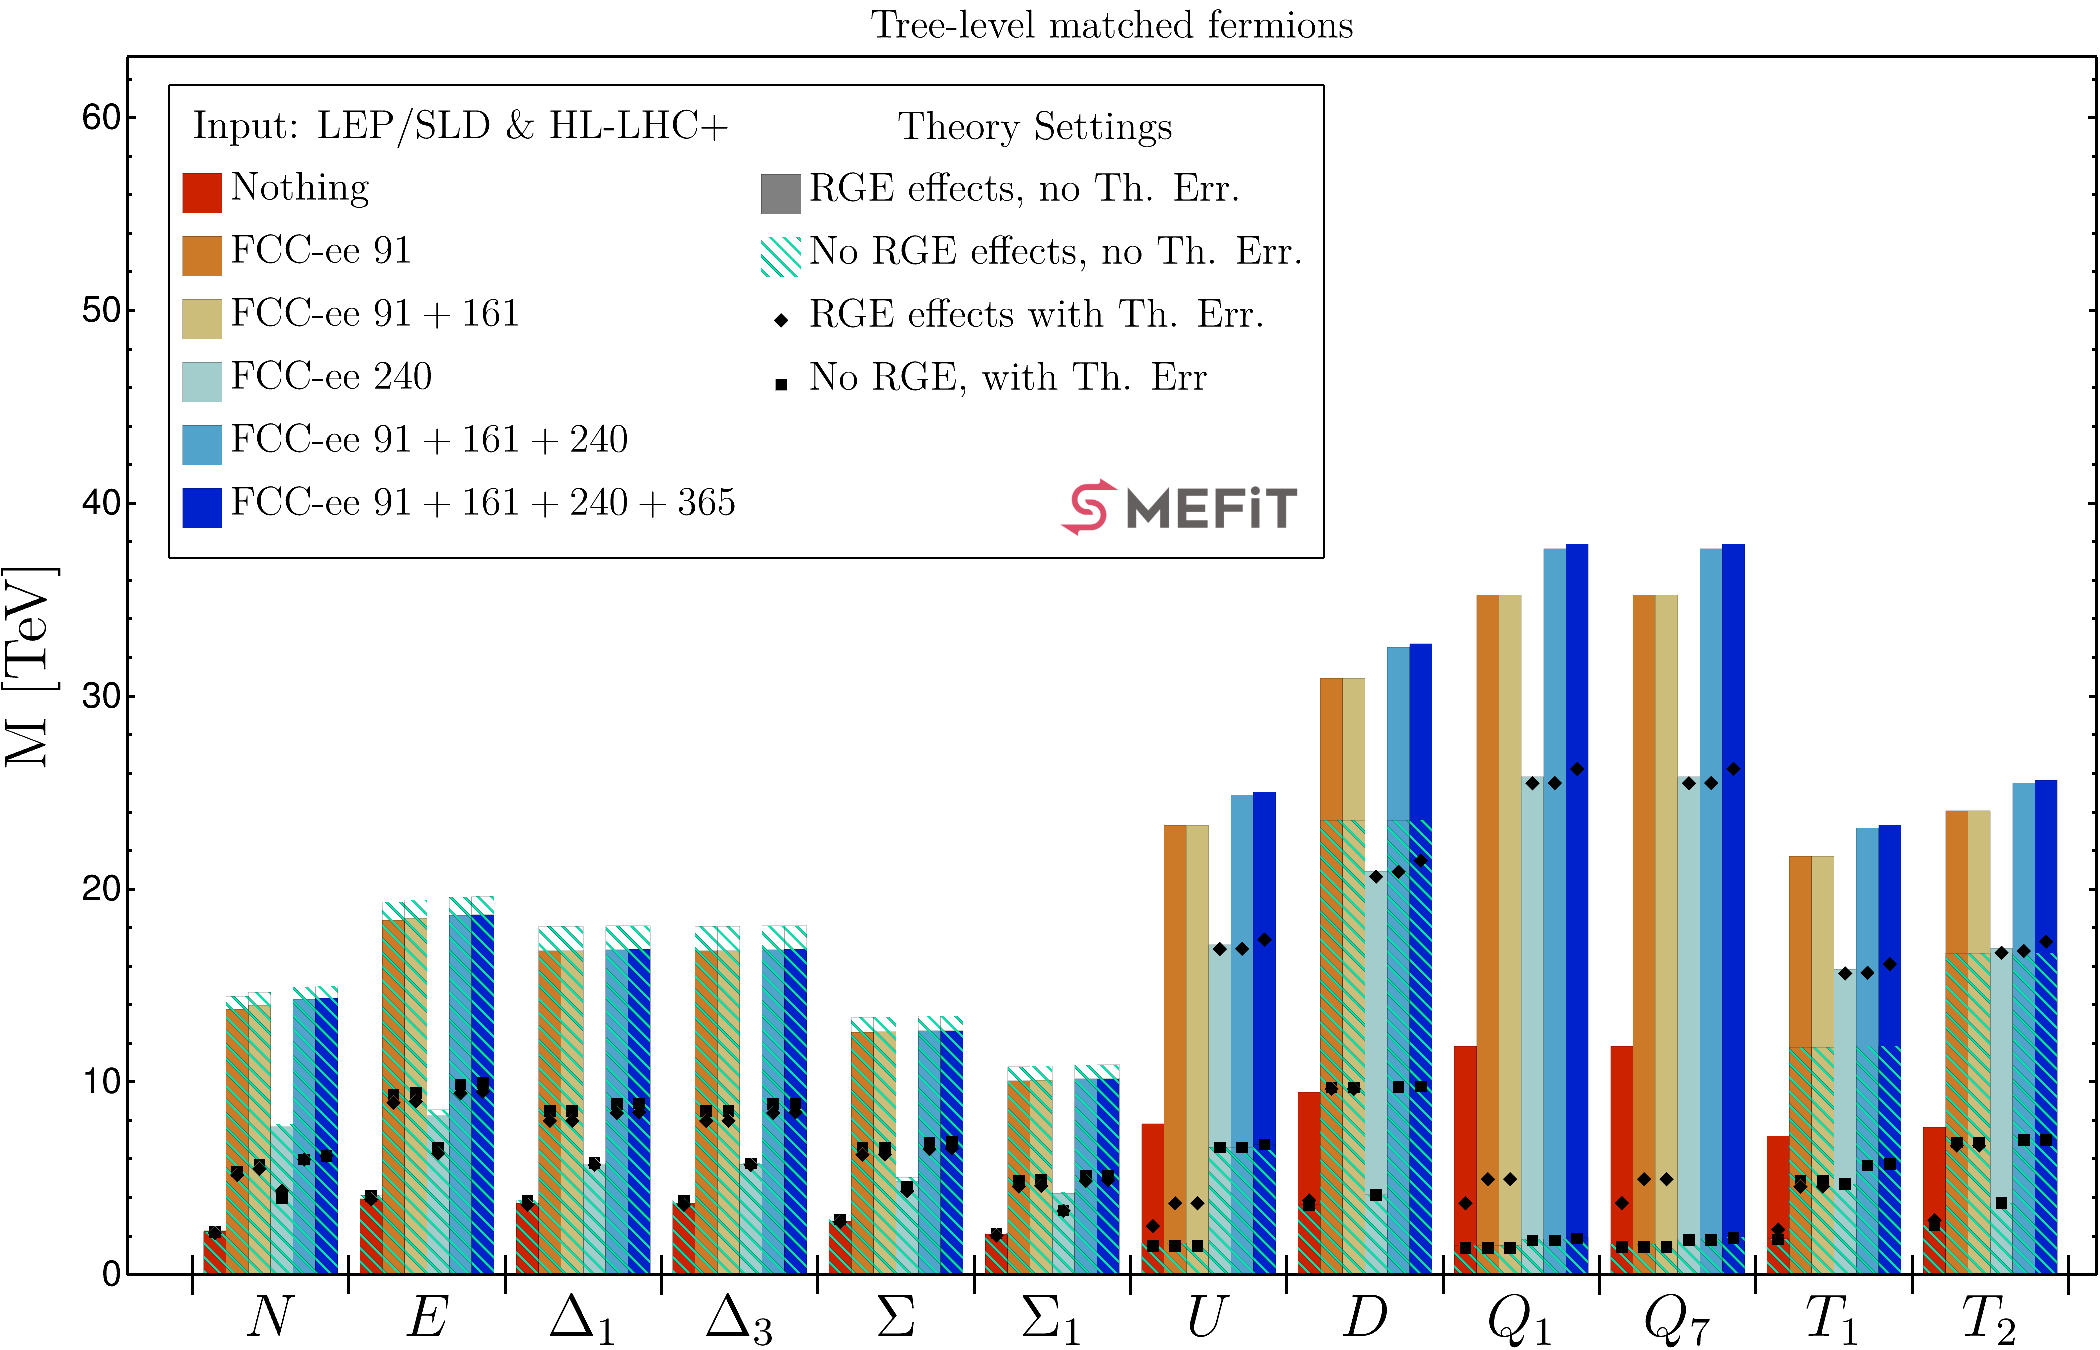
\includegraphics[width=0.65\linewidth]{PhysicsCase/Figs/plot_FCCFeasRep_runs_RGE_mass_UV_Fermions_FSR.pdf}
\caption{As Fig.~\ref{fig:SMEFITmatched}, but without the one-loop matched terms, for fermions.}
\label{fig:SMEFITfermions}
\end{figure}
\begin{figure}[ht]
\centering
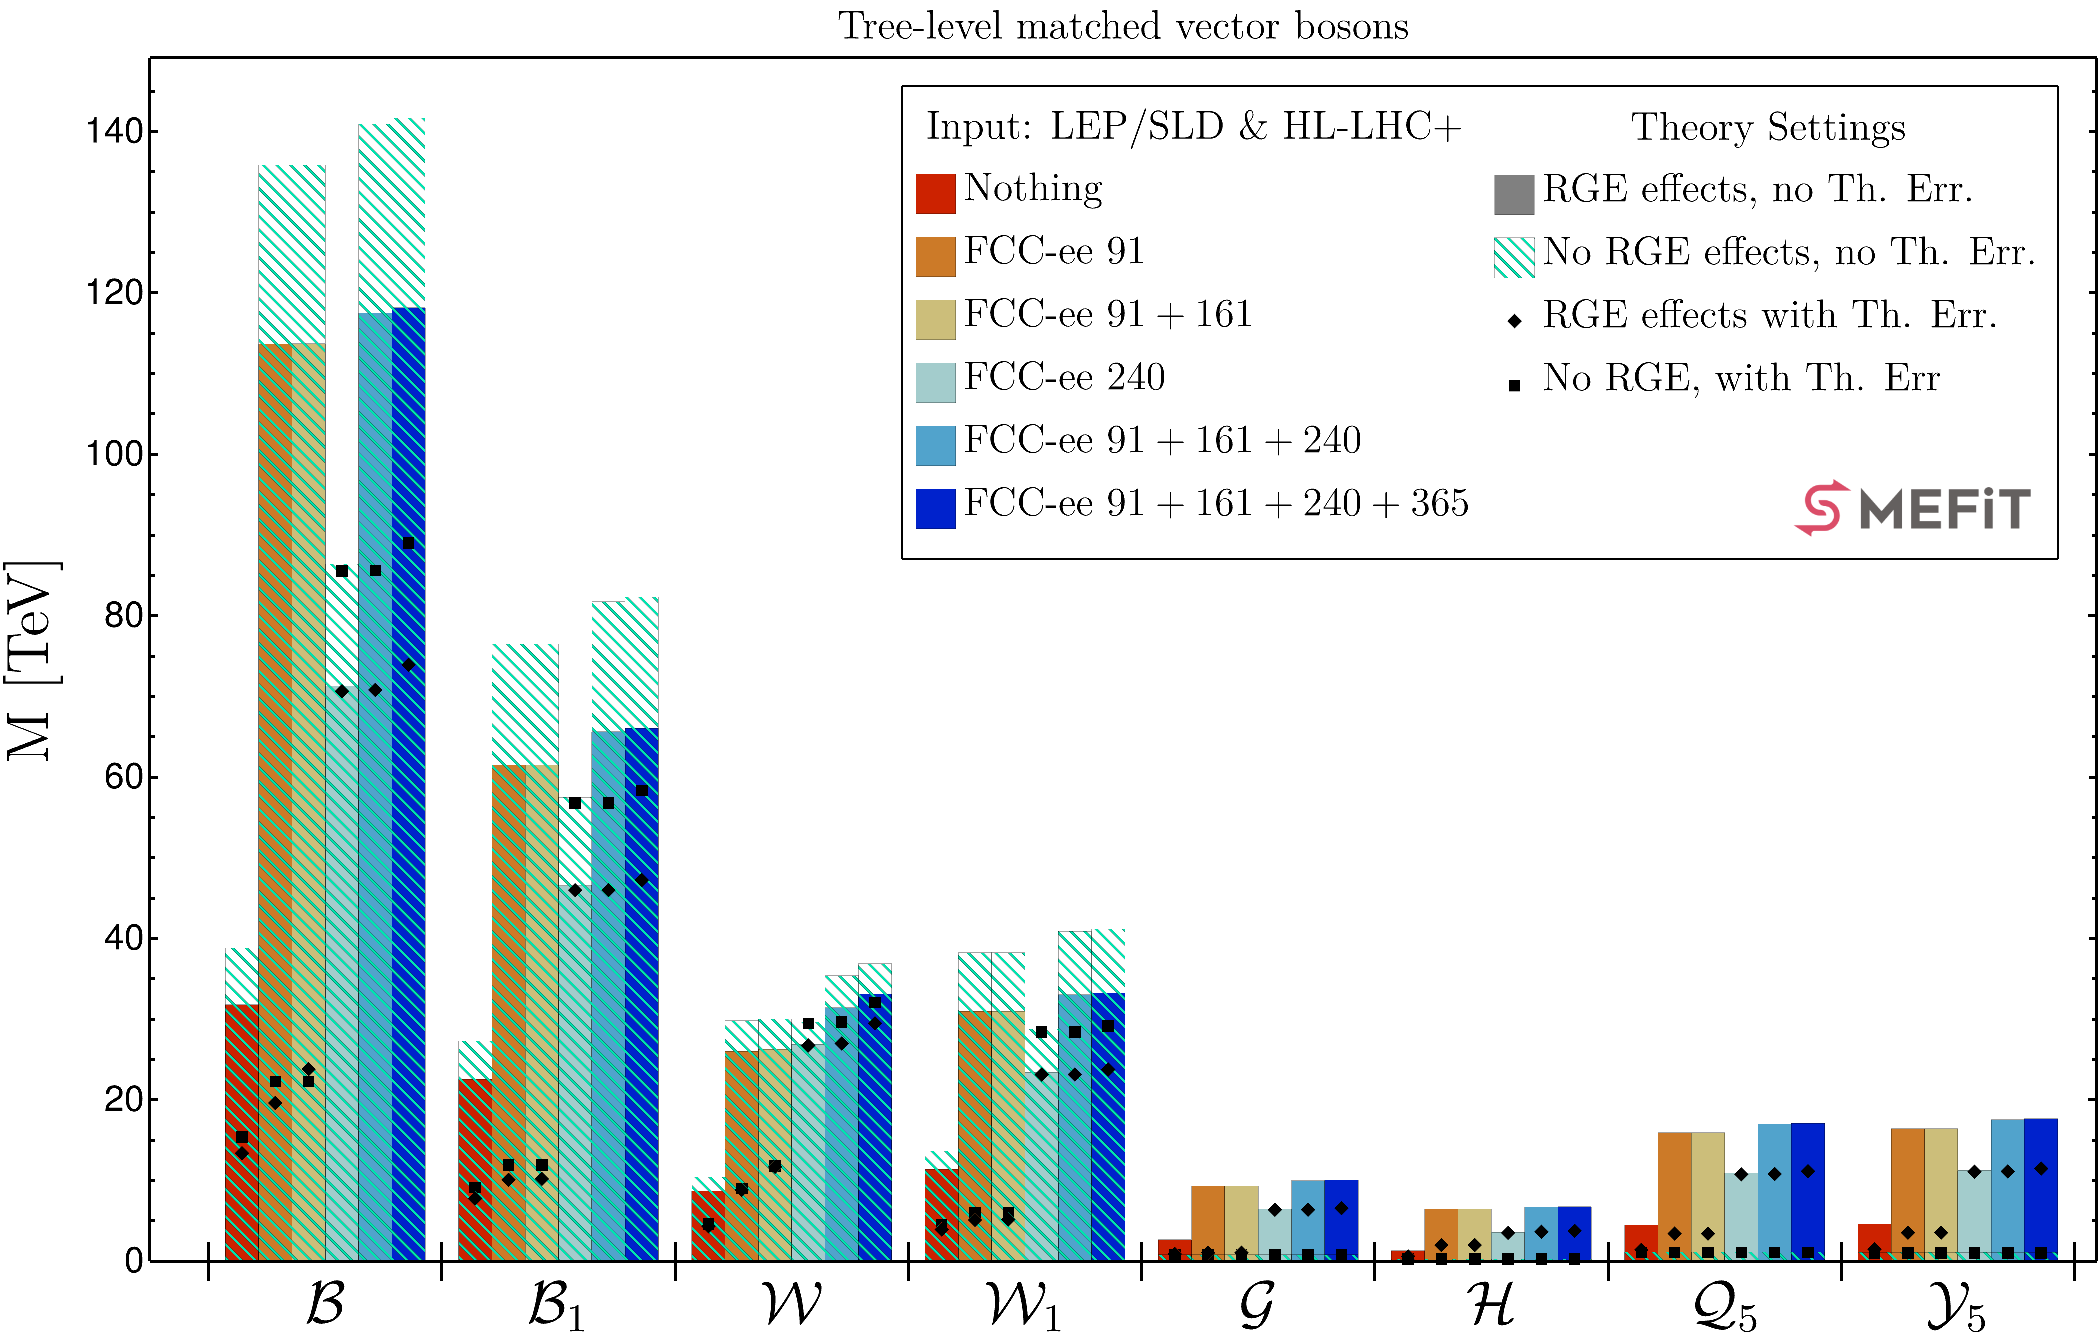
\includegraphics[width=0.85\linewidth]{PhysicsCase/Figs/plot_FCCFeasRep_runs_RGE_mass_UV_Vectors_FSR.pdf}
\caption{As Fig.~\ref{fig:SMEFITmatched}, but without the one-loop matched terms, for vectors.  
The models $\mathcal{B}$ and $\mathcal{W}$ include flavour-universal couplings to leptons. 
See Ref.~\cite{terHoeve:2023pvs} for details.}
\label{fig:SMEFITvectors}
\end{figure}

The picture that emerges from Figs.~\ref{fig:SMEFITmatched}, \ref{fig:SMEFITscalars}, \ref{fig:SMEFITfermions}, 
and~\ref{fig:SMEFITvectors} is that the \mbox{Tera-\PZ} programme of FCC-ee is, indeed, 
extremely powerful in searching for new physics, extending well beyond the scales probed at HL-LHC, 
and is also highly complementary to the Higgs run. 
The latter offers loop-induced sensitivity to the Higgs trilinear coupling~\cite{McCullough:2013rea}, 
which could probe custodially symmetric models, as shown for the $\Theta_1 + \Theta_3$ model in Fig.~\ref{fig:SMEFITmatched}. 
This weak custodial quadruplet scalar model and the Higgs trilinear coupling can, moreover, be probed on the \PZ pole, 
as shown on the left plot of Fig.~\ref{fig:custodialquadrupletandRSS}, 
with the combination significantly extending the coverage of the model parameter space~\cite{Maura:2024zxz}.

\begin{figure}[ht]
\centering
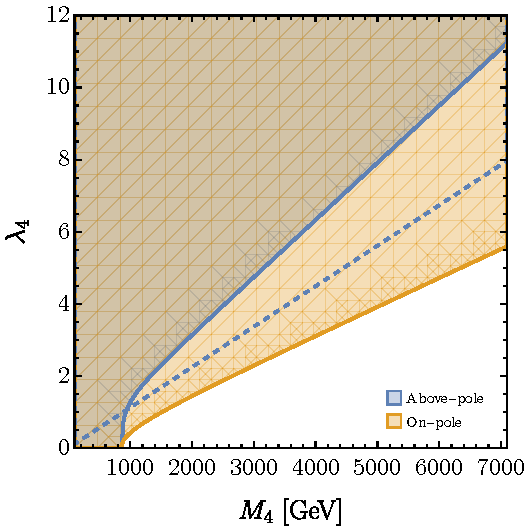
\includegraphics[width=0.4\linewidth]{Physics/PhysicsCase/Figs/CQplot.pdf}
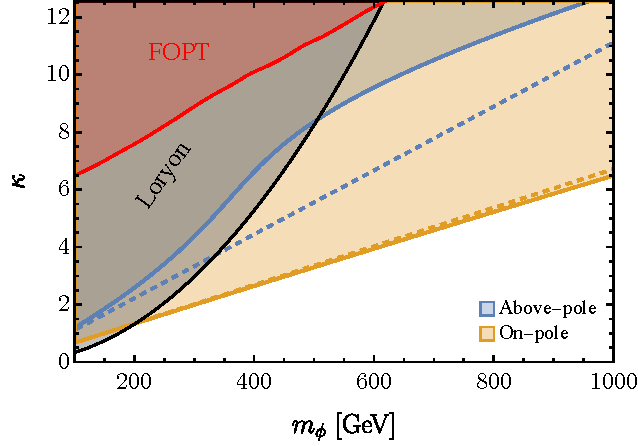
\includegraphics[width=0.55\linewidth]{Physics/PhysicsCase/Figs/RSSplot.pdf}
\caption{FCC-ee sensitivity at 68\% CL on the weak custodial quadruplet scalar (left) and real singlet scalar (right) models in the mass vs.\ coupling plane when combining \PZ pole data (orange) with $\PZ\PH$ measurements (blue). 
For the real singlet case, the constraints exclude a first order phase transition (FOPT) for the mass region shown. See Ref.~\cite{Maura:2024zxz} for further information. }
\label{fig:custodialquadrupletandRSS}
\end{figure}

The \mbox{Tera-\PZ} run is crucial to definitively answer the fundamental question of 
whether any particles other than the SM ones obtain most of their mass from the Higgs mechanism. 
Such so-called `loryon' candidates have a finite parameter space that can be almost entirely probed by current and future colliders, 
with a remaining open window for the elusive real singlet scalar model~\cite{Crawford:2024nun}. 
This window can potentially be closed by precision measurements at the \PZ pole, 
as shown on the right plot of Fig.~\ref{fig:custodialquadrupletandRSS}, from Ref.~\cite{Maura:2024zxz}, 
thus allowing this important question to be definitively settled. 
The high sensitivity of FCC-ee to the $\hat{W}$ and $\hat{Y}$ parameters, 
both at the \PZ pole and in higher energy runs, 
also enables constraining elusive BSM candidates, such as weakly interacting massive particles. 
The combination of on-pole and above-pole data, shown in Fig.~\ref{fig:wimps}, 
indeed gives a projected sensitivity beyond the indirect sensitivity reach of Drell--Yan searches at HL-LHC~\cite{Maura:2024zxz}. 

\begin{figure}[ht]
\centering
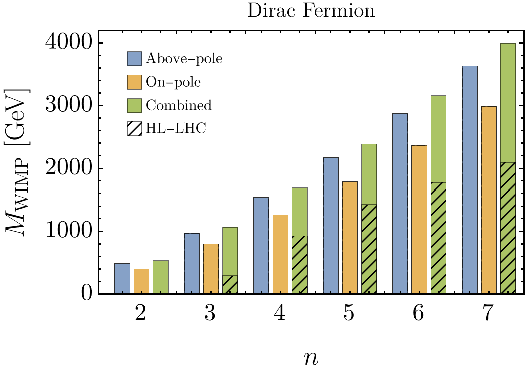
\includegraphics[width=0.49\linewidth]{Physics/PhysicsCase/Figs/WIMP_Dirac_fermion.pdf}
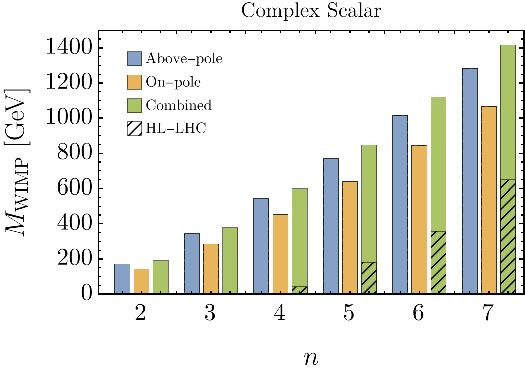
\includegraphics[width=0.49\linewidth]{Physics/PhysicsCase/Figs/WIMP_complex_scalar.pdf}
\caption{Projected 95\%~CL for $n$-plet Dirac fermion and complex scalar weakly interacting massive particles with zero hypercharge. 
From Ref.~\cite{Maura:2024zxz}.}
\label{fig:wimps}
\end{figure}

It will be critical to reduce theory uncertainties (Chapter~\ref{sec:theory}) 
in order to capitalise on the full potential of the FCC-ee data.  
Indeed, for a number of scenarios, 
the \mbox{Tera-\PZ} programme would probe the parameter space inaccessible to the runs at higher energies 
only in the context of improved theory uncertainties.  
An additional noteworthy aspect concerns the synergy with FCC-hh.  
Indirect probes at FCC-ee approach or exceed the 10\,TeV scale.
As a result, the only motivated successor to such a probe would be a collider capable of directly probing beyond that parameter space 
or one capable of directly producing the new states for which indirect evidence may have emerged at FCC-ee.  
In other words, a successor collider would necessarily have to be capable of directly probing beyond the 10\,TeV scale. 
The only such plausible facility is FCC-hh, strengthening the combined FCC physics case.

It should be noted that exceptions from the exploratory power of \mbox{Tera-\PZ} can exist.  
It was recently shown in Ref.~\cite{Davighi:2024syj} that a class of anomaly-free $\PZ^\prime$ models could exist 
in which the charge assignments lead to a suppression of electroweak-precision-sensitive operators at tree and one-loop level.  
Nonetheless, such a scenario would be strongly constrained above the \PZ-pole, 
both at FCC-ee and HL-LHC, demonstrating additional complementarity between runs and colliders.

The individual models considered are, themselves, not being proposed as well-motivated in any subjective sense.  
Rather, the collection of scenarios and the full family of Wilson coefficient patterns they populate 
can be taken as being qualitatively representative of the broad family of Wilson coefficients that could arise in UV scenarios.  
Thus the fact that the FCC-ee \mbox{Tera-\PZ} programme has sensitivity to this wide class of models, 
whether at tree-level or one-loop, is indicative of the fact that it will have sensitivity to generic UV scenarios.  
To argue otherwise would require the construction of an explicit counterexample model.  
Within the class of models considered in Ref.~\cite{Allwicher:2024sso}, 
the two counterexample states are $\Omega_4$ and a special case for $\mathcal{G}$, 
for which only the four top-right interaction is generated up to one loop. 
However, even BSM modifying four-top operators can be highly constrained through its next-to-leading-log running into the $T$ parameter 
at the \PZ pole~\cite{Allwicher:2023shc, Stefanek:2024kds}, 
as also seen in Figs.~\ref{fig:SMEFITscalars} and~\ref{fig:SMEFITvectors}.

Finally, as another concrete UV scenario, 
supersymmetric models are a well-motivated approach to understanding the origin of the Higgs and addressing the hierarchy problem, 
where the BSM particles are, instead, typically expected to arise from new weakly-coupled dynamics. 
The Higgs couplings at one loop, in particular to gluons and photons, 
can probe the contributions of superpartners such as the stop, the coloured scalar partner of the top. 
Such indirect probes are complementary to more model-dependent direct searches and their sensitivity can reach around a TeV, 
as shown on the left plot of Fig.~\ref{fig:susy}, taken from Ref.~\cite{Fan:2014axa}. 
The right plot of Fig.~\ref{fig:susy}, from Ref.~\cite{Knapen:2024bxw}, 
shows the projected \PZ branching ratio sensitivity at FCC-ee to the selectron and pure wino, 
together with the current direct search constraints at LHC.

\begin{figure}[ht]
\centering
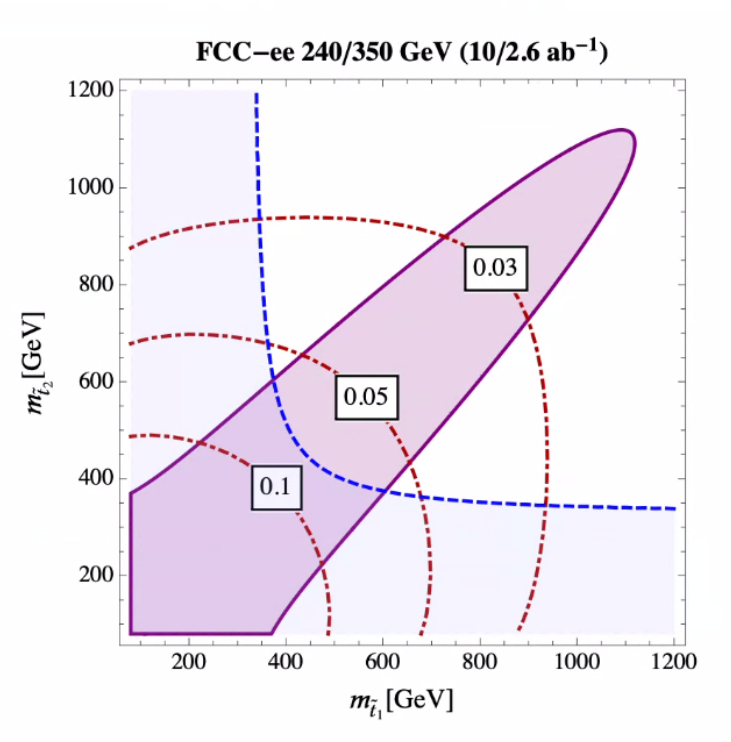
\includegraphics[width=0.4\linewidth]{PhysicsCase/Figs/susy_stop.jpeg}
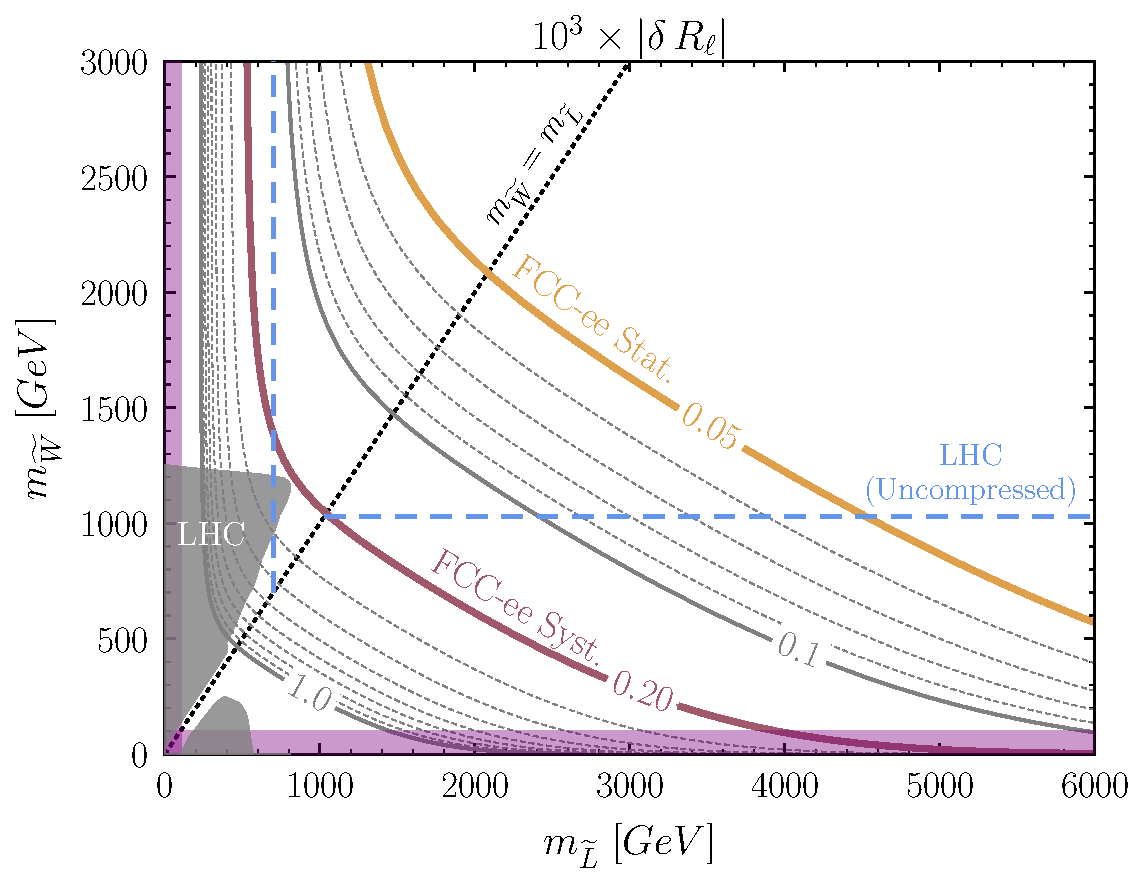
\includegraphics[width=0.5\linewidth]{PhysicsCase/Figs/delta_Rl_Wino_Linear_FSR.pdf}
\caption{Left: Projected 2\,$\sigma$ sensitivity of Higgs couplings to stops at FCC-ee 
in the parameter space of stop masses $m_{\tilde t_1}$ vs.\ $m_{\tilde t_2}$;
from Ref.~\cite{Fan:2014axa}. 
Right: FCC-ee \PZ branching ratio projected statistical and systematic 1\,$\sigma$ uncertainties 
in the left-handed selectron mass vs.\ pure wino mass plane;
from Ref.~\cite{Knapen:2024bxw} scaled to the baseline luminosities.}
\label{fig:susy}
\end{figure}

\subsubsection{Flavour deconstruction at FCC-ee}
\label{sec:otherBSM}

To give an example
of concrete scenarios explored through a combination of the unprecedented precision 
on \PZ-pole and $\PW\PW$-threshold observables with excellent capabilities as a flavour factory, 
a special class of theories based on `flavour deconstruction'~\cite{Davighi:2023iks} is considered, 
whereby part of the electroweak symmetry is resolved into three generation-specific copies $G_i$ 
(with the Higgs boson coupled to $G_3$). 
This symmetry, which arises, e.g., from gauge-flavour unification~\cite{Davighi:2022fer} 
or from extra-dimensions~\cite{Fuentes-Martin:2022xnb}, 
is broken to the SM in two steps that generate hierarchical fermion masses and mixings. 
The last breaking step, $G_{12} \times G_3 \to G$, 
should occur close to the TeV scale to avoid destabilising the Higgs potential, 
delivering TeV-mass gauge bosons in the adjoint of $G$ coupled mostly to the third generation. 

These electroweakly-charged and flavour non-universal gauge bosons give rise to a rich phenomenology 
across EWPOs, flavour observables, and high-energy LHC measurements,
which has been quantified by considering deconstructed hypercharge~\cite{Davighi:2023evx} 
and deconstructed $SU(2)_L$~\cite{Davighi:2023xqn} (Table~\ref{tab:pheno}). 
Firstly, EWPOs are shifted at tree-level because the heavy gauge bosons directly couple to the Higgs boson.
Constraints from LEP are already strong and the expected precision brought by FCC-ee would all but cover the `natural' regime 
in which these flavour models can be reconciled with the hierarchy problem. 
Secondly, being intrinsically non-universal theories of flavour, 
many rare \PB- and \PGt-decays receive tree-level shifts that will also be measured with excellent precision at \mbox{Tera-\PZ}.
While more detailed studies are needed to fully assess these prospects, 
key processes will be $\PB \to \PK^{(\ast)}\PGn\PAGn$, $\PQb \to \PQs\PGt\PGt$ transitions 
that are a unique opportunity at FCC-ee, and LFUV measurements in \PGt decays. 
In these models, the shift in $\PB \to \PK^{(\ast)}\PGn\PAGn$ 
is directly correlated to that in $\PBs \to \PGm\PGm$, 
which should be measured to few percent precision at HL-LHC~\cite{LHCb:2018roe}.
Lastly, these models are constrained by high-energy Drell--Yan measurements of $\Pp\Pp \to \ell\ell$, 
that should improve by nearly a factor of two after HL-LHC. 

Other flavour deconstruction models have been proposed where, for instance, 
a new force-carrying gauge boson field is associated with a TeV-scale $U(1)_{Y_3}$ $\PZ^\prime$, 
coupling primarily to the third family of fermionic fields~\cite{Allanach:2025wfi}.  
These models, currently favoured by measurements of \PB decays in tension with the SM predictions, 
can be thoroughly tested by FCC-ee.

To summarise, FCC-ee is an optimal machine for probing theories of flavour deconstruction 
because it achieves comparable sensitivity across diverse measurements 
traditionally separated into `electroweak' and `flavour' categories, 
but whose effects in such flavour models are inextricably tied. 
Viewing the electroweak and flavour programmes of FCC-ee together, 
and in combination with high-\pt and \mbox{low-\pt}  HL-LHC data, 
is therefore crucial to understanding its full power. 

\begin{table}[t]
\centering
\caption{Constraints from flavour, high \pt, and EWPOs 
on the mass of the gauge bosons predicted by flavour deconstruction.} 
\label{tab:pheno}
\begin{tabular}{c c c c}
\toprule
& Deconstructed $SU(2)_L$ & Deconstructed $U(1)_Y$ \\ \midrule
Electroweak: \PZ-pole \& $\PW\PW$-threshold & 9\,TeV (5\,TeV if exc.\ $m_{\PW}$) & 2\,TeV  \\
Flavour: $\PBs \to \PGm\PGm$ (up-alignment) & 7.5\,TeV & 2\,TeV \\
High \pt: Drell--Yan $\Pp\Pp \to \Pe\Pe, \PGm\PGm, \PGt\PGt$ & 4.5\,TeV & 3.5\,TeV \\ 
\midrule
EW projection FCC-ee & \multirow{2}{*}{30\,TeV} & \multirow{2}{*}{7\,TeV}\\
(on and above \PZ-pole \& \PW-pole)& & \\
\bottomrule
\end{tabular}
\end{table}

\subsubsection{Heavy Neutral Leptons}
\label{sec:HNL}

In its minimal version, the SM Lagrangian does not accommodate neutrino masses, 
but this historical accident can easily be overcome by minimally extending the SM. 
Nonzero neutrino masses offer many theoretical and phenomenological opportunities 
to address pending questions in the understanding of Nature.

Massive neutrinos can oscillate in flavour space, as experimentally observed since 1998. 
With three families, this phenomenon naturally leads to the possibility of breaking CP symmetry in the leptonic sector. 
Furthermore, fermion (or lepton) number violation might be observed. 
In the SM, fermion number conservation (FNC) stems from charge conservation for charged fermions
and from angular momentum conservation for massless neutrinos~\cite{Kayser:1989iu}. 
Thus, FNC is considered to be an accidental conservation law, which has no reason to hold if neutrinos are massive. 
The combination of the two possibilities opens the door to shedding light on the question of the existence of matter via leptogenesis.

When the FNC rule is relaxed, active neutrinos can mix with right-handed neutrinos, 
via Yukawa interactions mediated by the Higgs field. 
This minimal scenario is a concrete realisation of the (type-I) see-saw mechanism (Fig.~\ref{fig:Seesaw}). 
The right-handed neutrinos, which do not carry electric charge, weak isospin, or colour, 
have no interaction that would distinguish the particle from the antiparticle: they are naturally Majorana particles. 
At energies much below the Majorana mass, 
the mixing is described by an effective dimension-5 Weinberg operator that, 
after electroweak symmetry breaking, generates an effective mass for the active neutrinos. 
Having two mass terms for each family, the neutrinos undergo level splitting thus the `see-saw', 
with typically light active neutrinos and heavy sterile neutrinos.  
Unlike for other SM fermions, 
the Yukawa coupling is not proportional to the mass of the light neutrinos, 
but could either be made proportional to the geometric mean of the masses of the light and heavy particles, 
or be enhanced with a symmetry that protects the masses of the light neutrinos~\cite{Agrawal:2021dbo}. 
The resulting heavy mass eigenstates are called Heavy Neutral Leptons (HNLs) and are nearly sterile particles. 
The ensuing rich phenomenology includes the possible observation of LLPs, 
for which, in the mass range 20--80\,GeV, 
a thorough and conclusive search can be performed at FCC-ee, during the \mbox{Tera-\PZ} run.

\begin{figure}[ht]
\centering
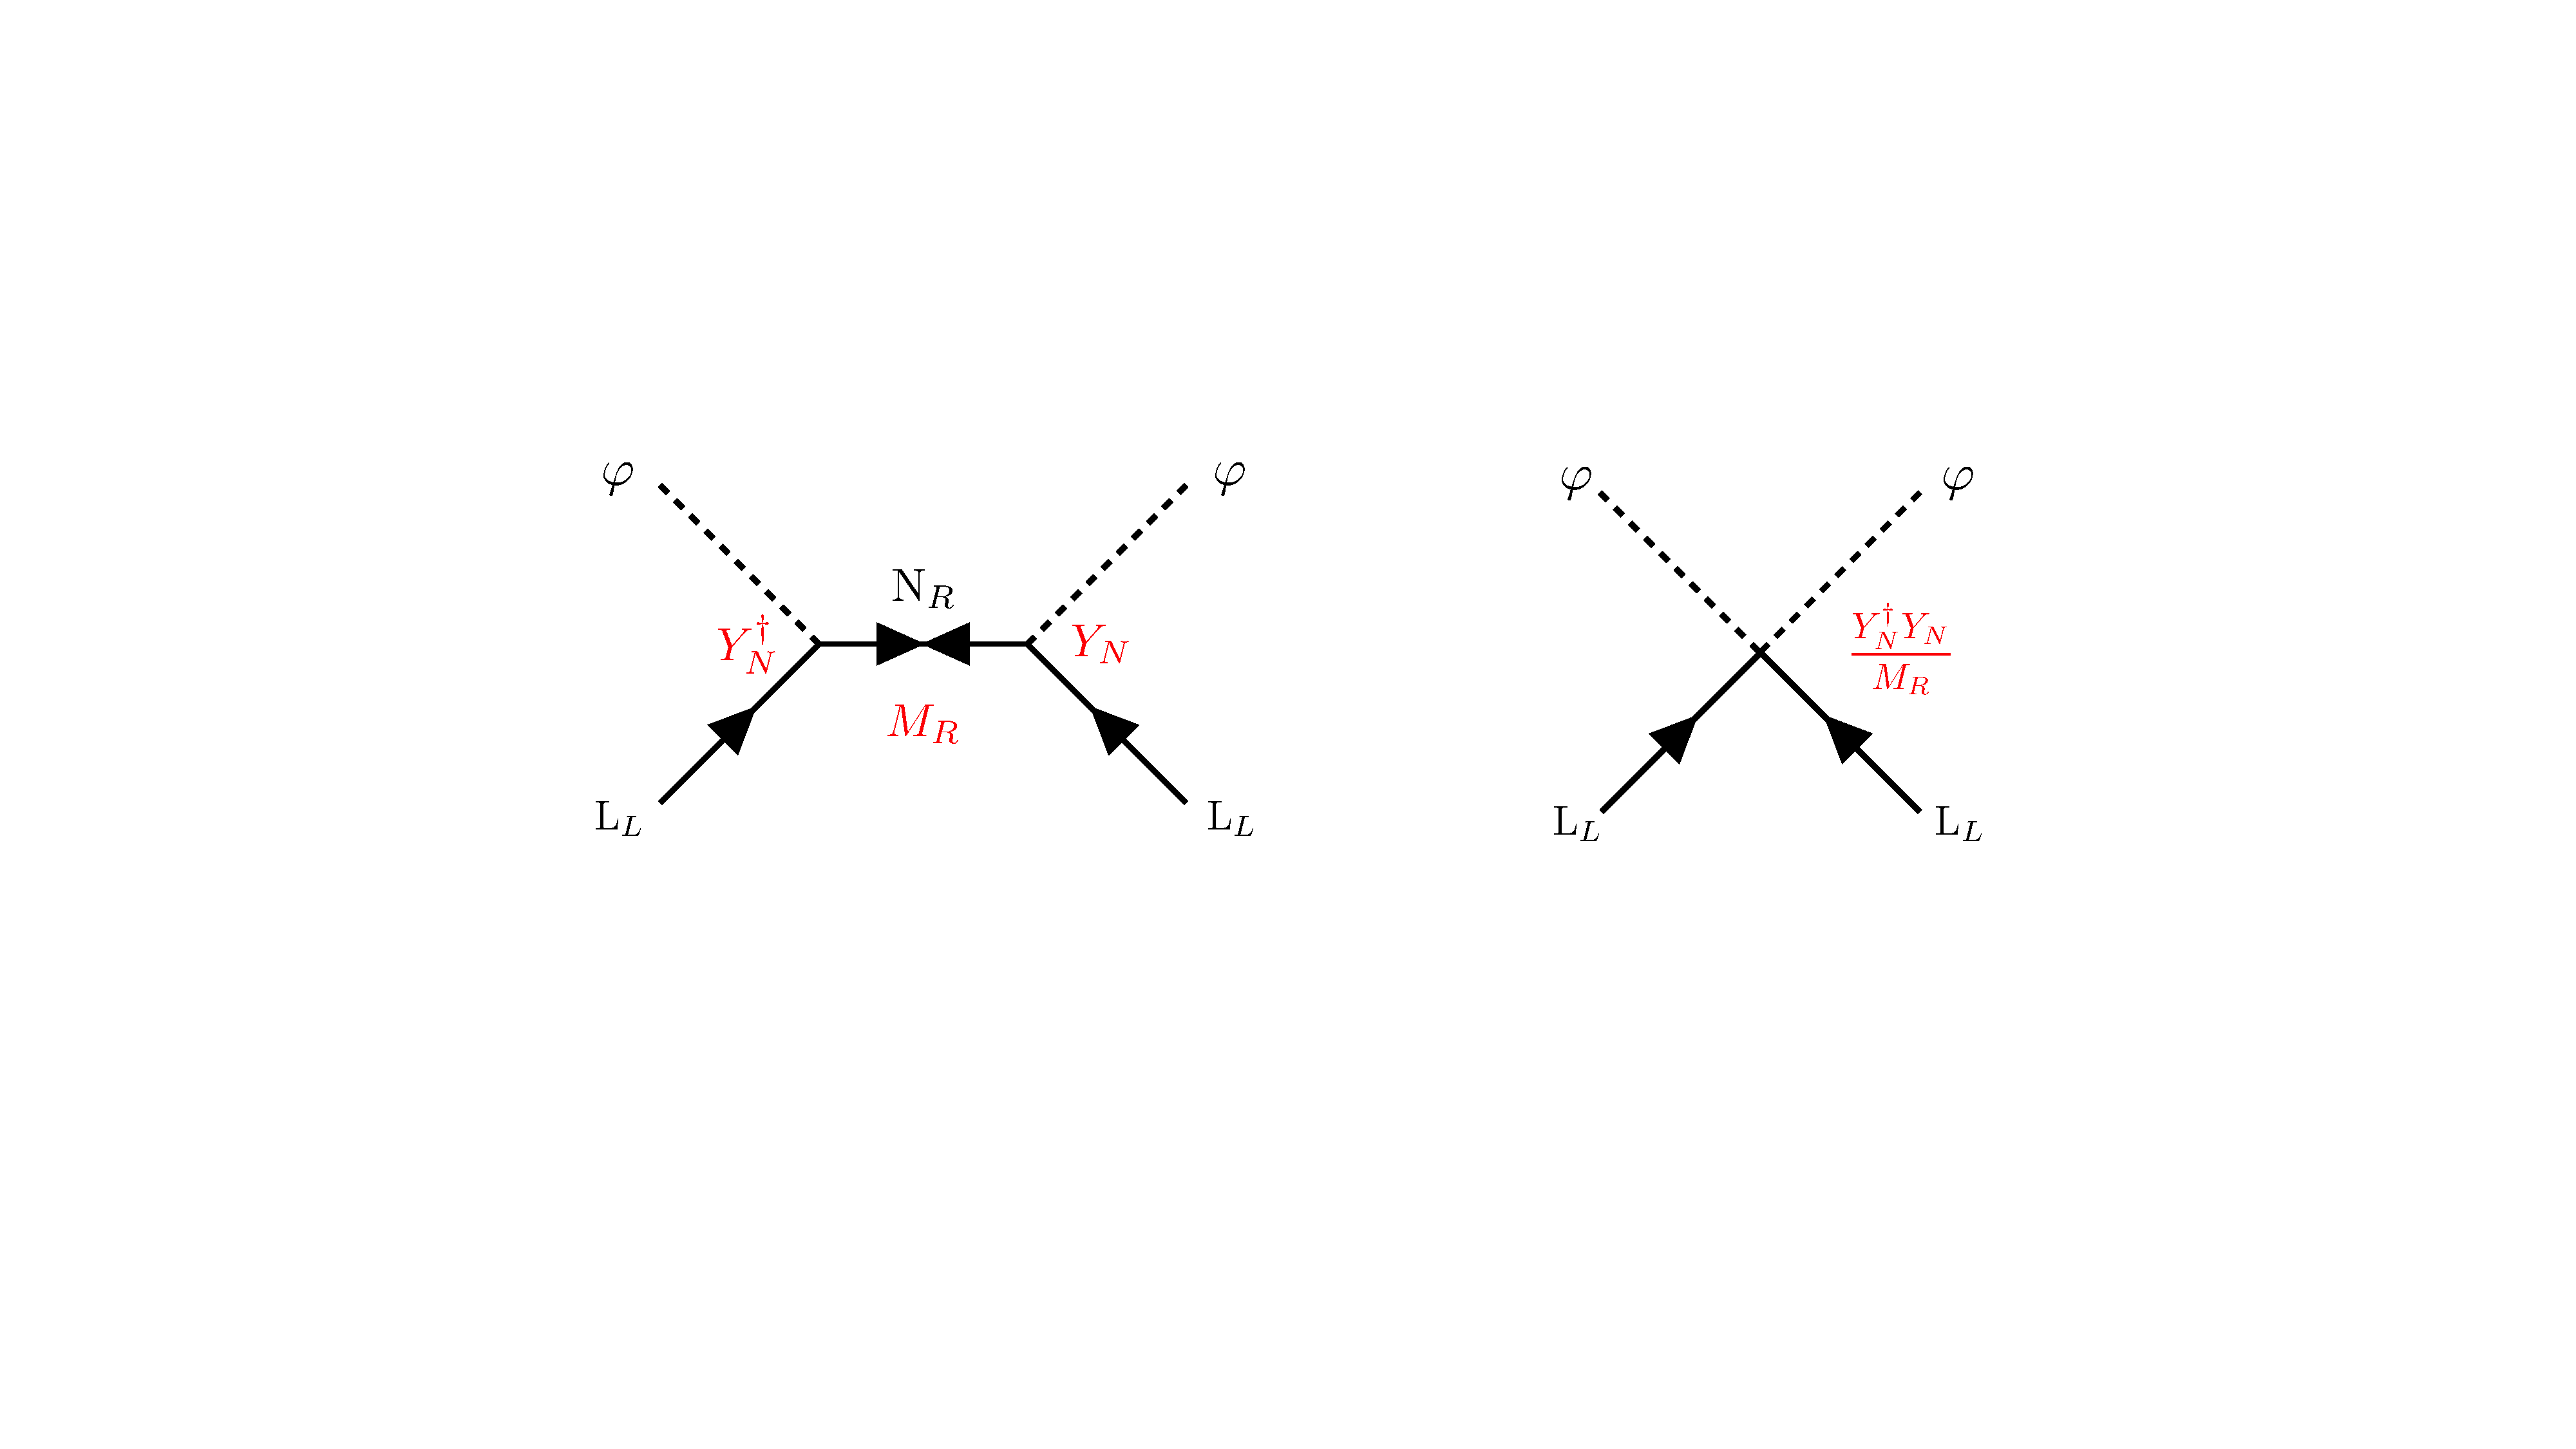
\includegraphics[width=25em]{PhysicsCase/Figs/TypeISeesaw_FSR.pdf} 
\caption{Schematic illustration of the type-I see-saw mechanism. 
Left: The left-handed lepton EW doublets $\mathrm{L}_L$ have Yukawa-like interactions $Y_N$, 
with the Higgs EW doublet $\varphi$, mediated by the heavy right-handed neutrinos $\mathrm{N}_R$. 
Right: At energies below the mass $M_R$ of these heavy neutrinos, 
an effective fermion-number-violating dimension-5 operator, 
involving two left-handed leptons and two Higgs fields, 
describes the low-energy degrees of freedom. 
After electroweak symmetry breaking, a Majorana mass is generated for the active left-handed neutrinos. 
This mass is proportional to the square of the original Yukawa coupling, 
to the squared Higgs vacuum expectation value $v$,
and to $1/M_R$. 
Heavy Neutral Leptons (HNLs), aligned with the right-handed neutrinos in the limit $M_R \gg v$, complete the spectrum.}
\label{fig:Seesaw}
\end{figure}

Generalising beyond this minimal scenario, FCC-ee can search for HNLs in the large sample of \PZ bosons produced resonantly. 
The \PZ decay to $\PGn_L + \text{HNL}$ followed by the decays of the heavy neutral lepton 
$\text{HNL} \to \ell + \PW^*$, 
$\text{HNL} \to \PGn + \PZ^*$, 
leads to a wealth of final state signatures that can be exploited at FCC-ee~\cite{Blondel:2014bra}. 
The \PZ branching ratio to HNLs is proportional to the squares of the mixing angles $U^2_{ij}$ between the SM neutrinos and the HNL, 
where $i,j$ run over the three neutrino flavours.

The very large number of \PZ boson decays allows the exploration of very low $U^2_{ij}$ values, for HNL masses below the \PZ mass. 
The explored values  may result in HNLs with a measurable path in the detectors, 
yielding spectacular signatures with jets or leptons produced far from the interaction vertex, with no SM backgrounds. 
In particular, for decay lengths in the detector between 1\,mm and 2\,m, 
a discovery would be possible for HNL masses up to 60--70\,GeV down to $U^2$ values of ${\cal O}(10^{-11})$. 
For larger HNL masses, up to the kinematic limit of the \PZ mass, a prompt analysis would be needed, 
which, because of significant SM backgrounds, would allow discovery for $U^2$ values of ${\cal O}(10^{-9})$.

Detailed simulation studies were performed to verify the experimental feasibility of these analyses 
and to determine the corresponding requirements on detector design. 
The reach in parameter space was first studied in a toy model commonly used to compare different experimental approaches, 
rather than a complete model for neutrino masses. 
The model features a single Majorana HNL mixing with a single flavour of active neutrinos. 
The signal samples and all of the SM decays of the \PZ boson, 
as well as four-fermion processes yielding the same final state as the HNL decays, 
were passed through a parametrised simulation of the IDEA detector (Chapter~\ref{sec:concepts}) and then analysed. 
Both semi-leptonic and fully leptonic decays of the HNL were studied, 
for the cases of mixing with an electron neutrino and with a muon neutrino. 
The fully leptonic decay mode provides a clean experimental final state, 
with a good reach for long-lived decays, but with a significant price in branching fraction. 
The semileptonic decay $\text{HNL} \to \ell \PGn j j$ has a branching fraction $\sim$\,50\%, 
allows full kinematic reconstruction of the neutrino decay, 
and was studied both for long-lived and prompt decays. 
The results are shown in Fig.~\ref{fig:hnlreach} and documented in 
Refs.~\cite{MSc_Moulin, MSc_Critchley, note_HNL_Polesello_Valle_mujj,Blondel:2022qqo, 
note_HNL_Presilla_Giappichini,note_HNL_Williams}. 

\begin{figure}[ht]
\centering

\includegraphics[width=0.8\textwidth]{PhysicsCase/Figs/fcc_lines_LLP_FSR.pdf}
\caption{Discovery potential in the $m_{N}-|U_{\mu N}|^2$ plane. 
The FCC-ee potential is based on the decay channel $\text{HNL} \to \ell \PGn j j$ 
and is shown as a red (green) line for the prompt (long-lived) analyses described in the text. 
The blue line shows the reach of a search for long-lived particles in the decay channel $\text{HNL} \to \PGmp\PGmm \PGn$.
The dashed green line bounds the area where, out of $6 \times 10^{12}$ \PZ bosons, 
three events are produced with visible HNL decays inside an FCC-ee detector, 
i.e., with a displacement smaller than 5\,m
and larger than 0.5\,mm (based on the analytical formulas in Ref.~\cite{Drewes:2022rsk}).
The requirement to explain the light neutrino masses imposes a lower bound, indicated as a pink band,  
on the total HNL mixing (summed over flavours). 
The width of this band indicates the uncertainty in this lower bound 
due to the current lack of knowledge about the absolute scale and the ordering of the light neutrino masses. 
Light neutrino oscillation data can be explained anywhere above this band, 
in particular in models where the neutrino masses are protected by a symmetry related to approximate lepton-number conservation. 
Furthermore, this region could also accommodate the observed matter-antimatter asymmetry 
via a leptogenesis mechanism~\cite{Drewes:2021nqr}. 
The existing limits from LHC searches are shown as turquoise areas. 
The expected discovery potential of projected experimental searches based on long baseline experiments 
are shown as green areas and are taken from the website accompanying Ref.~\cite{Antel:2023hkf}, 
where all the original works are cited.}
\label{fig:hnlreach}
\end{figure}

The conclusion of these studies is that searches at FCC-ee enable the HNL discovery 
over a mass range beyond the reach of specialised detectors for LLP searches being developed for HL-LHC 
and for mixing values much smaller than those covered by future searches at HL-LHC, 
for both prompt and long-lived signatures. 
Besides the work based on parametrised detector simulations, 
the model is also being studied~\cite{note_HNL_CLD_Andrea} 
through a detailed \textsc{Geant4} simulation of the ILD detector (Chapter~\ref{sec:concepts}).

The models featuring a single HNL are useful for assessing, in a simplified way, the parameter space coverage of the experiments. 
In order to explain the observed neutrino oscillations, however, at least two HNLs are needed. 
A realistic model~\cite{Tastet:2021vwp} featuring two Majorana neutrinos with coupling to all three flavours of active neutrinos 
was studied in the fully leptonic final state featuring two electrons or muons in the final state. 
The patterns of couplings were chosen such as to be compatible with neutrino oscillation data 
based on the benchmarks proposed in Ref.~\cite{Abdullahi:2022jlv}. 
As for the single-neutrino analyses, 
the study was performed with the parametrised simulation of the IDEA detector and featured a full background analysis. 
An estimate of the reach was obtained for different coupling scenarios, 
corresponding to both normal and inverted neutrino mass hierarchy.

The phenomenology of the `Symmetry Protected Seesaw Scenario'~\cite{Shaposhnikov:2006nn, Kersten:2007vk} 
has been presented in Refs.~\cite{Antusch:2016ejd, Antusch:2022ceb}. 
This model adds two right-chiral neutrinos, required to explain the observed light neutrino mass squared differences, 
provided with a protective lepton number-like symmetry (LNLS) 
to ensure that the two heavy neutral leptons form an almost degenerate pair of pseudo-Dirac neutrinos.
The main phenomenological signature of this model is the production of lepton flavour violating final states, 
with a probability that oscillates with the length of the flight path of the HNL in the detector~\cite{Antusch:2023jsa}. 
The region in parameter space where this oscillation would be detectable at FCC-ee 
is mapped in detail in the phenomenological study documented in Ref.~\cite{Antusch:2024otj}. 
An experimental study was performed based on this work, 
with the same parametrised detector simulation and software as the studies described above~\cite{note_HNL_Polesello_Valle}. 
For HNL masses below 35\,GeV, for favourable ratios of the HNL width and of the mass difference between the two pseudo-Dirac states, 
a striking oscillation signal would be observed, allowing the measurement of the mass difference.

A large fraction of the model parameter space consistent with the see-saw mechanism, 
including those with symmetry-enhanced neutrino masses, 
such as the inverse~\cite{Mohapatra:1986bd} or linear~\cite{Akhmedov:1995ip,Akhmedov:1995vm} models, 
would be probed. 
For masses around 40\,GeV, the FCC-ee sensitivity would reach the smallest value of the mixing angle 
theoretically compatible with the mass range experimentally still allowed for the active neutrinos.

With HNLs (as well as with other light and feebly-coupled particles, such as ALPs), 
FCC-ee is simultaneously a discovery and a precision tool, in a single collider. 
In view of the cost and time scales associated with the construction of each new collider, 
such an advantage cannot be overstated.
Indeed, the number of HNLs that can be detected during the \PZ-pole run 
grows as $|U_{\ell N}|^4$ if their decay length in the laboratory exceeds the detector size, 
or as $|U_{\ell N}|^2$ if it is smaller than the effective detector dimensions
As a direct consequence, 
up to a million HNL decays can be observed during the \mbox{\PZ-pole} run
if $|U_{\ell N}|$ is near the current upper experimental limits~\cite{Drewes:2022rsk}. 
%
Such a large sample opens the way for the measurement of several quantities, 
from which important information about the underlying particle physics model can be extracted,
as the following.
\textit{i)}~The branching ratios of HNL decays into different SM generations 
can be measured with per-cent accuracy~\cite{Antusch:2017pkq}, 
which allows the consistency with neutrino oscillation data to be checked;
many parameters of the see-saw model to be constrained~\cite{Drewes:2024bla} 
(including CP-violating phases and the absolute neutrino mass scale); 
the leptogenesis hypothesis~\cite{Antusch:2017pkq} to be tested; 
and underlying flavour and CP symmetries~\cite{Drewes:2024pad} to be probed.
\textit{ii)}~The number of HNL events and the measurement of the HNL lifetime 
can reveal information about the violation of lepton number~\cite{Blondel:2022qqo,Drewes:2022rsk} 
as well as underlying flavour and CP symmetries~\cite{Drewes:2024pad}.
\textit{iii)}~Finally, the angular distribution and the energy spectrum of the HNL decay products 
can provide information regarding the lepton number violation~\cite{Blondel:2021mss} 
and the HNL mass splitting~\cite{Antusch:2023jsa,Antusch:2024otj,note_HNL_Polesello_Valle}.

The combination of these observables may provide important information about the HNL role in particle physics and cosmology, 
in particular in the context of neutrino masses and leptogenesis. 
It can also shed light on the properties of the underlying particle-physics theory 
within which the see-saw model is embedded (such as flavour and CP symmetries). 

\subsubsection{Dark matter and dark sectors}
\label{sec:dark}

Understanding the origin\,/\,nature of dark matter (DM) is a central question in contemporary physics, 
connecting particle physics and astrophysics. 
Despite decades of searches across experiments, the favoured DM candidates, the WIMPs, have not been found, 
and the lower bounds on their masses are progressively pushed beyond the reach of TeV-class $\epem$ colliders.

Mono-photon searches at FCC-ee can play a significant role in probing the so far unexplored parameter range 
allowed by the WIMP relic density constraints~\cite{Horigome:2021qof}.  
In particular, predictive models of leptophilic candidates with a thermal origin can be tested.  
Missing energy signatures at FCC-ee can probe much of the parameter space 
for which DM direct annihilation into a dilepton yields the observed relic density 
in Higgs-like models with mass-proportional couplings to charged leptons~\cite{Cesarotti:2024rbh}. 
Models of asymmetric dark matter can also be probed at FCC-ee, 
with a sensitivity to DM-lepton interactions improved by almost an order of magnitude~\cite{Roy:2024ear}. 
Additionally, it would be possible to detect spin 0, 1, and~1/2 DM at FCC-ee 
in the context of simple, consistent, and renormalisable field theories 
that provide the correct DM abundance and satisfy direct detection, indirect detection, 
and collider constraints~\cite{Grzadkowski:2020frj}. 

Hidden sectors, consisting of new, invisible particles that interact almost imperceptibly with the SM, 
are rapidly gaining attention as they could hold the answer, 
not only to the dark matter problem but also to a variety of other open questions in the field. 
The dark sector could contain a multitude of hidden particles. 
After all, the visible sector is non-minimal, 
so there is no good reason why the dark sector should contain only one type of dark matter particle and nothing else. 
Benefiting from a clean environment, high luminosity, and large acceptance, 
FCC-ee can directly scrutinise the $\mathcal{O}$(1--100)\,GeV mass range for 
so-far unknown particles, with interactions that would otherwise have been too feeble to detect. 

Dark sectors typically exhibit a stable particle, fundamental or composite, that could be a DM candidate, 
and one or more mediator particles coupled to the SM via a neutral portal. 
The spin of the mediator particle defines the portal: 
vector, e.g., dark photon; 
scalar or pseudoscalar, e.g., Higgs portal; 
or fermion, e.g., sterile neutrino. 
These well-motivated dark sectors can be thoroughly explored at FCC-ee 
in a mass-coupling range that is inaccessible by any other means with the same sensitivity. 
Furthermore, small couplings of dark sector particles to SM particles could give rise to LLPs 
and other unconventional collider signatures, such as dark showers.  

Dark photons may mix kinetically with the SM hypercharge gauge boson. 
This possibility can be studied in $\epem \to \mathrm{A}^\prime \gamma$ production, 
where the dark photon A$^\prime$ decays to $\PGmp\PGmm$. 
The sensitivity to small coupling values could be significant, 
reaching around $\sim$\,$2 \times 10^{-4}$ for $m_\mathrm{A^\prime}$ ranging from 10 to 80\,GeV at FCC-ee~\cite{Karliner:2015tga}. 
Alternatively, dark photons or dark $\PZ^\prime$ bosons can also be investigated 
via $\epem \to \mathrm{A}^\prime \PH$ or $\PZ^\prime \PH$ production at the $\PW\PW$ threshold or above~\cite{Giffin:2020jtl}.

Finally, the associated production of a neutrino and a dark sector fermion can also be searched for at FCC-ee 
in mono-photon signatures~\cite{Ge:2023wye}. 
This kind of search has sensitivity up to mass values in excess of 1\,TeV. 
Other searches, such as invisible decays of a dark Higgs boson~\cite{Haghighat:2022qyh}
or \PZ boson decays to an invisible dark photon~\cite{Cobal:2020hmk} can also be exploited.

\subsubsection{Axion-like particles}
\label{sec:alps}

Axion-like particles (ALPs) are generically expected in many BSM extensions, 
most famously in QCD axion models originally introduced to tackle the strong CP problem~\cite{Bauer:2018uxu}. 
In these models, ALPs can be heavier than the QCD axion and serve as mediators to the dark sector. 
Astrophysical and beam-dump experiments constrain the ALP-photon coupling at low masses, 
but are less stringent in the 0.1--100\,GeV range~\cite{Agrawal:2021dbo,dEnterria:2021ljz}, 
potentially accessible at FCC-ee via $\epem \to \axion \gamma$~\cite{Bauer:2018uxu} 
and $\epem \overset{\gamma\gamma}{\longrightarrow} (\epem) \axion$~\cite{RebelloTeles:2023uig}, 
with the ALP $\axion$ decaying as $\axion \to \gamma\gamma$. 
Various aspects of the ALP phenomenology at FCC-ee are addressed 
in Refs.~\cite{Cheung:2023nzg,Calibbi:2022izs,Liu:2022tqn,Zhang:2021sio}

The FCC-ee sensitivity to the $\epem \to \axion \gamma$ channel was studied in Ref.~\cite{note_ALP_Polesello} 
with the parametrised simulation of the IDEA detector.
Two final states were addressed: 
the `prompt' case, where the ALP decays near the interaction vertex, 
and the `monojet' case, where the ALP decays outside the detector, 
yielding the signature of a monochromatic photon recoiling against missing energy and mass. 
For both channels, a full kinematic analysis was developed to separate the signal from irreducible SM backgrounds.

Sensitivity to photon couplings down to $<10^{-3}$\,TeV$^{-1}$ can be obtained at FCC-ee 
in the $m_\axion$ range from 0.1 to 100\,GeV, 
extending current limits by more than two orders of magnitude in the \mbox{Tera-\PZ} run. 
In particular, the `monophoton' signature would cover a difficult region in the vicinity of 1\,GeV, 
which is not accessible to beam dump experiments. 
In an intermediate region in mass and at small coupling values, 
the ALP lifetime is large enough to give rise to measurable paths inside the detector, 
providing LLP signatures that could be accessible by exploiting the pointing capabilities of the calorimeters.

The ALP coupling to \PZ and Higgs bosons can also be probed via $\epem \to \PZ \axion$ or $\PH\axion$, 
with visible \PZ boson decays or $\PH \to \PQb\PAQb$, 
and either $\axion \to \gamma\gamma$ or $\axion \to \ell^+\ell^-$. 
Decays to SM particles other than photons are less constrained and provide an additional opportunity for ALP discovery at FCC-ee.
A preliminary study of the sensitivity of FCC-ee to ALPs decaying into two gluons is presented in Ref.~\cite{note_ALP_Andrea}.

The projected sensitivity of the ALP search is illustrated in Fig.~\ref{fig:axion}, 
where the importance of FCC-ee is conspicuous in probing ALPs coupling to photons 
with a lifetime below cosmological/astrophysical scales, i.e., with a mass above 1\,MeV. 

\begin{figure}[ht]
\centering
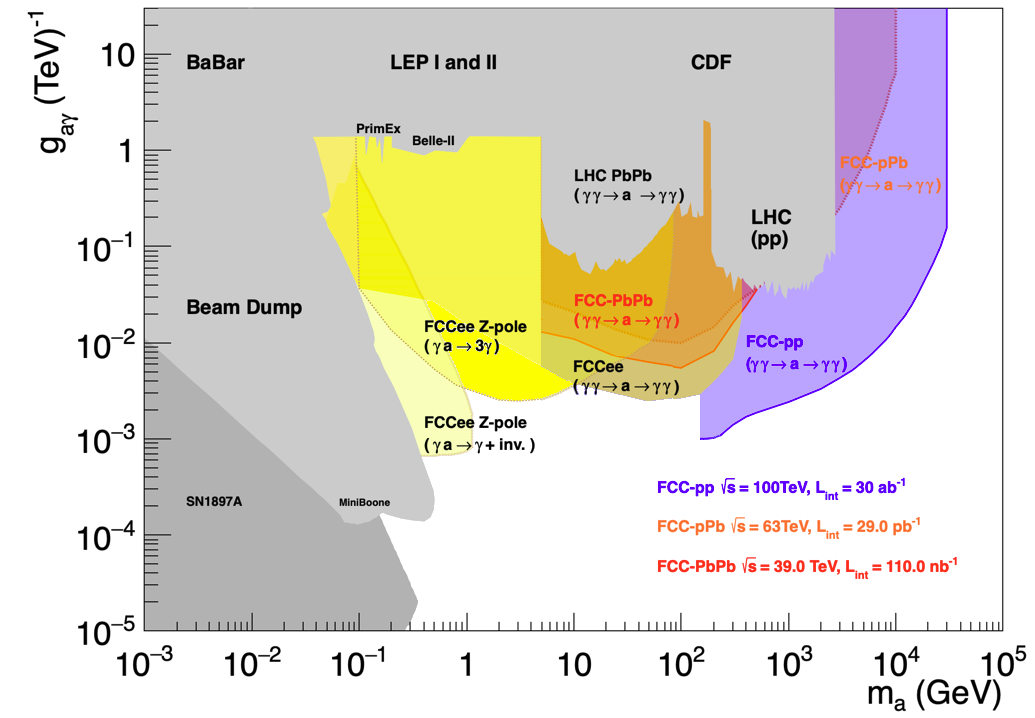
\includegraphics[width=\linewidth]{PhysicsCase/Figs/alp_final_FCCeehh_col_FSR.png}
\caption{Projected sensitivity for ALPs in the photon coupling vs.\ ALP mass plane 
from the three following processes at FCC-ee: 
$\epem \to \gamma \axion \to 3\gamma$ (yellow area),  
photon-fusion $\gamma\gamma \to  \axion \to 2\gamma$ (salmon area)~\cite{RebelloTeles:2023uig},
and $\epem \to \gamma \axion \to \gamma + \text{INV}$ (orange area). 
Existing limits (in grey) are adapted from Refs.~\cite{Agrawal:2021dbo,Antel:2023hkf}. Also shown are projected exclusion limits at 95\% C.L. on the ALP-photon coupling as a function of the ALP mass expected from searches for $\gamma\gamma\to \axion \to \gamma\gamma$ in pp (violet), pPb (dark pink), and PbPb (orange) collisions at FCC-hh \cite{PRebello_DdE25}.}
\label{fig:axion}
\end{figure}

\subsubsection{Exotic decays of the Higgs and \texorpdfstring{\PZ}{Z} bosons}
\label{sec:exoHZ}

The large Higgs boson event sample at FCC-ee allows a direct search for exotic decays of the Higgs boson. 
Exotic decays are predicted by a variety of BSM theories~\cite{Curtin:2013fra, Cepeda:2021rql,Ma:2020mjz, Alipour-Fard:2018lsf}, 
including extended scalar sectors, SUSY, and dark sector models with Higgs or vector portals. 
Higgs branching ratios up to four orders of magnitude lower than the expected HL-LHC reach will be probed at FCC-ee,
giving access to entirely new channels~\cite{Liu:2016zki}. 
  
Substantial work in preparing searches for Higgs boson decays into long-lived particles (LLPs) is ongoing,  
focusing on signatures with displaced vertices~\cite{note_LLPs_ExoticHiggsDecays}. 
The results suggest that FCC-ee is sensitive to long-lived scalars with decay lengths of order 1\,mm to 10\,m, 
with the peak sensitivity for decay lengths around 0.3\,m, as shown in Fig.~\ref{fig:HiggsLLP}. 
Additional studies, 
comparing different detector setups for exotic Higgs decays, 
have also been initiated~\cite{note_exoticHiggs_Larson}.

\begin{figure}[ht]
\centering
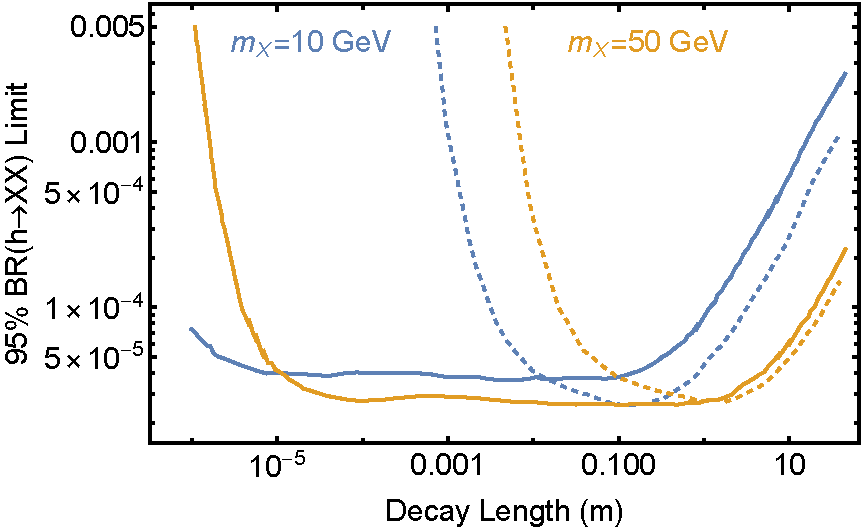
\includegraphics[width=0.7\linewidth]{PhysicsCase/Figs/ExoticHiggsLLP_FSR.pdf}
\caption{Estimate of the sensitivity to LLPs in exotic Higgs portal decays; adapted from Ref.~\cite{Alipour-Fard:2018lsf}. 
Solid (dashed) lines correspond to dedicated light (heavy) LLP search strategies.}
\label{fig:HiggsLLP}
\end{figure}

Searches for exotic \PZ decays to LLPs can also be carried out at FCC-ee during the \PZ pole run. 
In models of $R$-parity-violating supersymmetry, studied in Ref.~\cite{Wang:2019orr}, 
the FCC-ee sensitivity to long-lived light neutralinos in \PZ decays exceeds that of hadron colliders 
or of future dedicated LLP experiments by three orders of magnitude.
Comparable gains in sensitivity can be obtained in other searches, such as \PZ decays into hidden mesons~\cite{Cheng:2019yai}.

The available parameter space of new SM-neutral vector bosons (${\PZ}^\prime$) that couple exclusively to leptons 
could be significantly extended, 
offering the best performance of all future collider projects in the kinematically allowed mass range 
(from 5 to 360\,GeV)~\cite{GonzalezSuarez:2024dsp}.

In brief, by taking full advantage of the large \mbox{Tera-\PZ} event samples, 
the dark sector programme at FCC-ee extends the intensity-frontier discovery potential significantly. 
It provides access to very-weakly-interacting dark-sector particles 
with couplings so small that they are usually considered typical of beam-dump experiments, 
but in a mass range wholly inaccessible to any other intensity-frontier experiment.  
Given that there is no preferred mass range for such states, 
this mass-range extension by more than two orders of magnitude provides unique scientific opportunities in particle physics.

\subsubsection{Other new physics searches}

Other possible studies at FCC-ee include, for example, 
searches for lepton-flavour violation (LFV) in different 
manners~\cite{Hajahmad:2024arh,Munbodh:2024shg,Altmannshofer:2023tsa,Ho:2022ipo,Calibbi:2021pyh,Kamenik:2023hvi}, 
compositeness~\cite{Stefanek:2024kds}, leptoquarks~\cite{Crivellin:2020ukd}, 
new scalars~\cite{magnan2024}, 
and more.   
In this instance, the production of hidden-valley light quarks would perturb the QCD cascade, 
generating correlations among the final state particles that are absent in the SM.  
A detailed experimental study is in progress.  

\subsubsection{Complementarity and synergy between FCC-ee and FCC-hh}

The FCC-hh will complement and substantially extend the FCC-ee physics reach in nearly all possible directions. 
The seven-fold centre-of-mass energy increase with respect to LHC 
enhances the potential for observing new particles at mass scales up to 40\,TeV, as shown in Fig.~\ref{fig:schannel}. 
Indirectly, it will be sensitive to energies well above its kinematic reach of 100\,TeV, 
for example in the tails of Drell--Yan distributions. 
Should any deviations from SM expectations be observed at FCC-ee, FCC-hh has the potential to pinpoint its microscopic origin.  
Some specific synergies between FCC-ee and FCC-hh in this regard are highlighted in the next paragraphs.

\begin{figure}[ht]
\centering
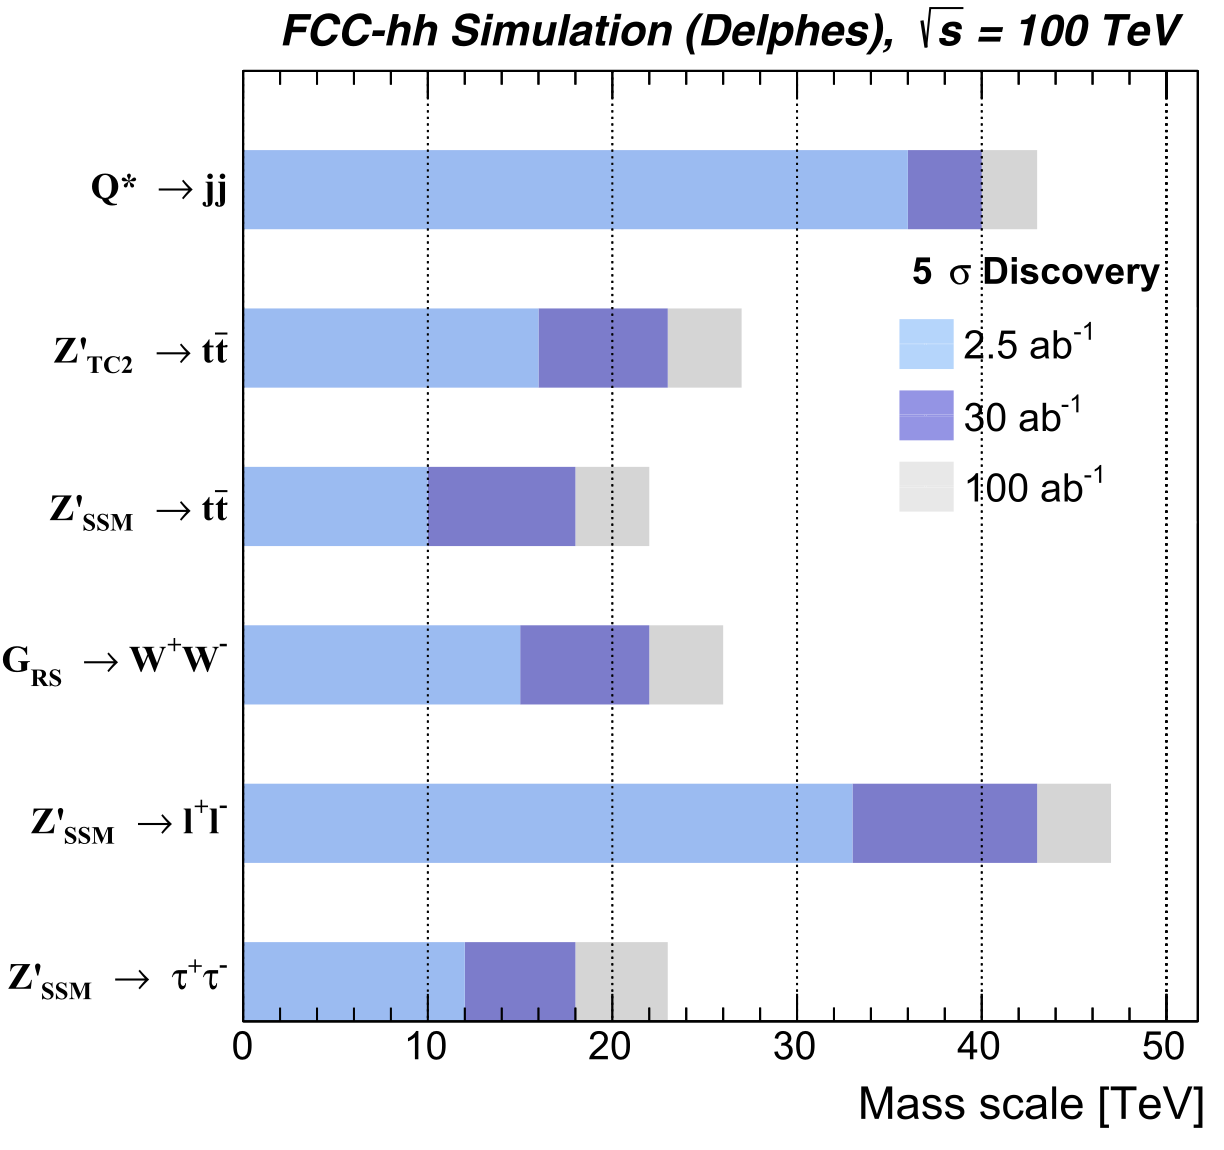
\includegraphics[width=0.6\linewidth]{PhysicsCase/Figs/FCCHHschannelreach.png}
\caption{Summary of the 5\,$\sigma$ discovery reach, 
as a function of the resonance mass, for different FCC-hh luminosity scenarios. 
From Ref.~\cite{Helsens:2019bfw}.}
\label{fig:schannel}
\end{figure}

As already alluded to in Section~\ref{sec:PhysicsCaseHiggsEW}, 
there are many synergies between FCC-ee and FCC-hh that come together 
to make the integrated FCC physics programme more than the sum of its parts. 
For example, the absolute determinations of Higgs couplings and its total width at FCC-ee 
is necessary to fully exploit the potential of FCC-hh that is only able to measure relative coupling ratios. 
The clean environment of FCC-ee enables the precise determination of SM parameters necessary to reduce uncertainties for FCC-hh. 
Moreover, certain types of BSM physics can only be accessed by FCC-ee and not FCC-hh, and vice versa.   
For instance, the nature of the electroweak phase transition will be probed by the precise measurement of the Higgs self-coupling 
and the search for additional Higgs partners at FCC-hh, together with potential deviations in the Higgs couplings at FCC-ee.

More concretely, if a deviation in $\kappa_{\PZ}$ were observed at the level of 0.5\%,  
this hint would be less than half of one sigma at HL-LHC (with some unavoidable assumptions), 
but would correspond to an unambiguous 5\,$\sigma$ discovery at FCC-ee.  
In Ref.~\cite{Abu-Ajamieh:2020yqi}, 
it was shown that for a BSM modification of this coupling 
new physics would have to show up at an energy scale of 
\begin{equation}
E_{\text{Max}} \simeq \frac{1.1 \text{TeV}}{\sqrt{|\kappa_Z-1|}} \, .
\end{equation}
Thus, a deviation of 5\,$\sigma$ at FCC-ee would correspond to an energy scale of 15\,TeV, 
essentially guaranteeing that FCC-hh would be able to discover the heavy states 
ultimately responsible for the low energy Higgs coupling deviation, 
illustrating a compelling, dynamic, interplay between FCC-ee and FCC-hh.

This synergy also extends to astrophysics and cosmology. 
Beyond-the-Standard-Model physics leading to a phase transition of some new sector, 
anywhere from the electroweak to the TeV scale, 
could yield gravitational wave signatures accessible to the next-generation gravitational wave observatories, 
such as LISA, the origin of which could then potentially be directly accessed at FCC-hh~\cite{Friedrich:2022cak}. 
The detection of high-energy gamma rays in astrophysical observatories such as CTA~\cite{Montanari:2022buj} 
may be due to a TeV-scale WIMP, 
but with a large degree of uncertainty inherent to such indirect observation methods. 
The FCC-hh will be directly sensitive to the entire upper mass range,
of around 1 and 3\,TeV for triplet and doublet thermal WIMP dark matter, respectively~\cite{fcc-phys-cdr}, 
far beyond the reach of any conventional dark matter direct detection experiment, as illustrated in Fig.~\ref{fig:DM}. 
Cosmic-ray physics will furthermore benefit from hadron collision data at unprecedented energy and luminosity. 

\begin{figure}[ht]
\centering
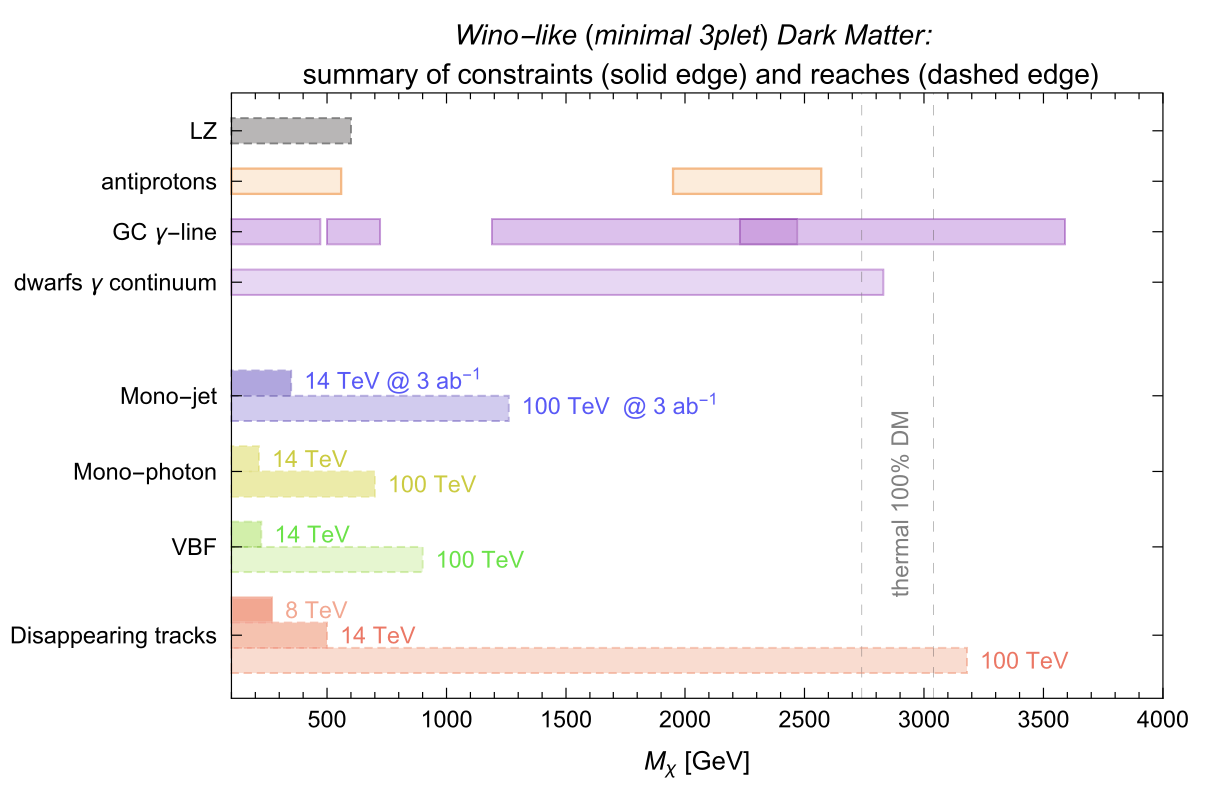
\includegraphics[width=1.0\linewidth]{PhysicsCase/Figs/Wino.png}
\caption{The projected sensitivity of searches for a WIMP triplet DM candidate 
in final states with disappearing tracks at FCC-hh~\cite{fcc-phys-cdr}.
Adapted from Ref.~\cite{Cirelli:2014dsa}.}
\label{fig:DM}
\end{figure}

The multiplicity of partons in the proton makes FCC-hh the most versatile high-energy parton collider 
for the broadest possible exploration of elementary particle processes. 
Similarly to LHC, its capabilities may be augmented by hosting complementary detectors for 
neutrino physics, dark sectors, and long-lived particles that may otherwise escape undetected.   
Together, FCC-ee and FCC-hh can truly enter the tens of TeV scale, indirectly and directly, 
to fully explore the open questions that LHC has only begun to touch upon. 

\subsection{Selected topics in flavour physics}
\label{sec:PhysicsCaseFlavour}

The peculiar structure of quark and lepton masses, as well as the quark mixing angles, 
is ad~hoc within the SM and is likely the low-energy imprint of some new dynamics. 
This structure implies approximate flavour symmetries that give rise to the strong suppression 
of a series of flavour-changing processes within the SM,  
whose precise experimental study allows probing dynamics at scales well above the electroweak scale.  
It is necessary to push the precision flavour frontier further and the FCC-ee programme offers unique opportunities in this respect.
Despite the fact that many tests in this sector have been performed in the recent past, 
without reporting significant deviations from the SM, the discovery potential remains high.

One class of unique opportunities concerns \PQb-hadron and \PGt decays, and, in particular, $\PQb \to \PGt$ transitions. 
These processes directly test models where 
new physics is coupled mainly to the third generation 
--- a general feature of many explicit BSM scenarios. 
Moreover, the class of models that can be tested indirectly via such studies 
is also the one less constrained by direct searches (given the suppressed couplings to light quarks). 
Here, the FCC-ee programme offers a particularly large margin of improvement 
over the accuracy expected from currently approved flavour physics experiments, 
both at HL-LHC and at lower-energy $\epem$ colliders (in particular Belle~II at Super~KEKB).
The key features of the flavour-physics programme during the \PZ-pole run at FCC-ee can be summarised as follows.

\begin{itemize}
\item \emph{Clean environment} (as in \PB-factories), 
with momentum and tagging efficiency of the pair-produced \PQb's, \PQc's, and \PGt's from \PZ decays, 
with $\sim$\,10 times more $\bbbar$ and $\ccbar$ pairs than the total collected by Belle~II (Table~\ref{tab:flavouryields}).
\item \emph{Boosted \PQb's and \PGt's}, leading to a significantly higher efficiency (compared to \PB-factories) 
for modes with missing energy (especially multiple-\PGn modes) and inclusive modes, 
as well as smaller uncertainties in lepton ID efficiencies.  
\end{itemize}

\begin{table}[ht]
\centering
\caption{Yields of heavy-flavoured particles produced at FCC-ee for $6 \times 10^{12}$ \PZ decays~\cite{Monteil:2021ith}.} 
\label{tab:flavouryields}
\begin{tabular}{c ccccccc} 
\toprule
Particle species & \PBz & \PBp & \PBzs & \PGLb & \PBpc & $\PQc\PAQc$ & $\PGtm\PGtp$ \\
\midrule
Yield ($\times 10^9$)    & 370 &  370 &  90  & 80 & 2 & 720 & 200 \\
\bottomrule
\end{tabular} 
\end{table}

These features lead to to the identification of the following class of observables as particularly promising: 
i)~neutral-current rare \PQb- and \PQc-hadron decays with $\PGtp\PGtm$ and $\PGn\PAGn$ pairs in the final state; 
ii)~charged-current \PQb-hadron decays with a $\PGt\PGn$ pair in the final state; 
iii)~CP-violating observables in \PQb- and \PQc-hadron decays involving neutral particles in the final states 
(\PGpz, \PKS, \PGg, \ldots);  
iv)~lepton flavour violating \PGt decays; 
v)~precision tests of lepton universality in \PGt decays.

In addition to these \emph{classical} flavour studies via low-energy probes, 
a truly unique opportunity offered by FCC-ee is the possibility of 
determining flavour parameters from \PW decays,
as well as searching for flavour-violating decays of \PZ and Higgs bosons. 
Within the SM, these processes are possibly too rare to be detected, 
but their search is an effective way to constrain or discover BSM dynamics. 
Some further ideas uniquely relevant to the FCC-ee flavour programme 
are discussed in Refs.~\cite{Grossman:2021xfq,Chrzaszcz:2021nuk, Monteil:2021ith}

The wide-ranging FCC-ee flavour physics programme cannot be easily summarised in a few pages. 
The most interesting classes of observables are listed below, 
together with a discussion of a few examples that illustrate the physics reach and the diversity of this programme.

\subsubsection{Lepton universality tests in \texorpdfstring{\PGt}{tau} decays} 

The major improvement expected at FCC-ee in the precision of measurements of 
the leptonic \PGt decay branching fraction, the \PGt mass, $m_\PGt$, and the \PGt lifetime, $\tau_{\PGt}$, 
corresponds to a jump of more than one order of magnitude (from $10^{-3}$ to $10^{-4}$) 
in tests of universality between third-generation and light leptons~\cite{Lusiani:2018zvr, Dam:2018rfz}.
An illustration of the FCC-ee reach on these measurements is shown in the left panel of Fig.~\ref{fig:tauLFU}~\cite{Lusiani:2024tau}. 
With this level of precision, 
models addressing the hint of non-universality observed in $\PQb \to \PQc \PGt \PGn$ decays~\cite{Allwicher:2021ndi} 
could either be unambiguously confirmed, leading to a major discovery, or ruled out. 
Theoretical work (on electroweak and radiative corrections), achievable with present knowledge but not yet available, 
is needed to reduce the theoretical systematic uncertainties on these measurements 
well below the projected experimental systematic uncertainties. 

\begin{figure}[ht]
\centering 
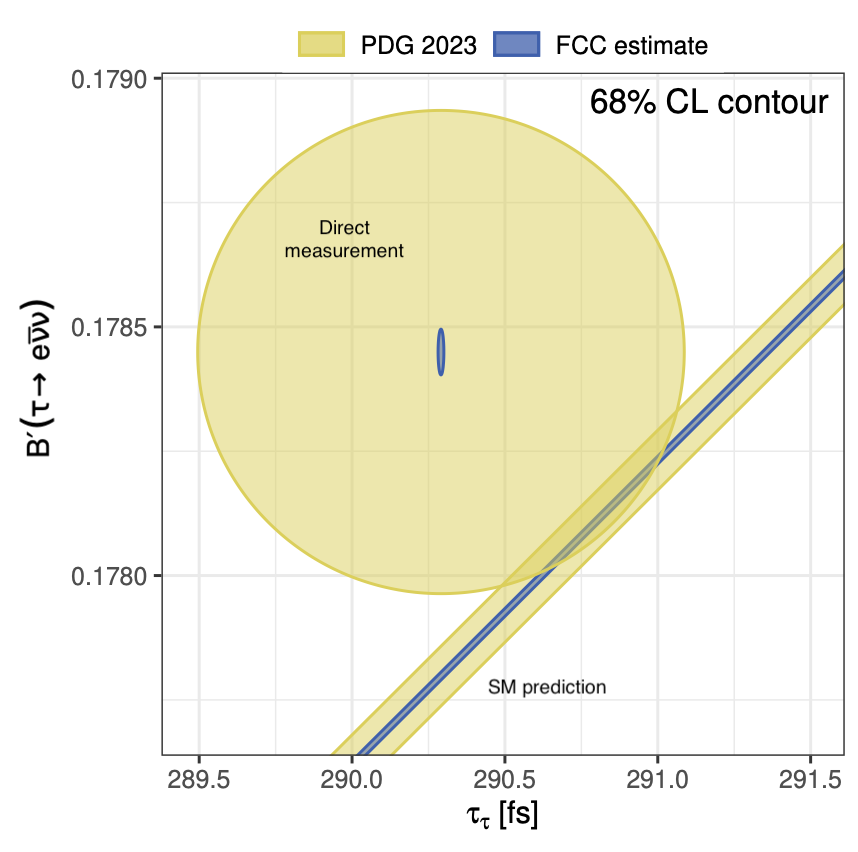
\includegraphics[width=0.4\textwidth]{Physics/PhysicsCase/Figs/tau_LFU_exp.png}
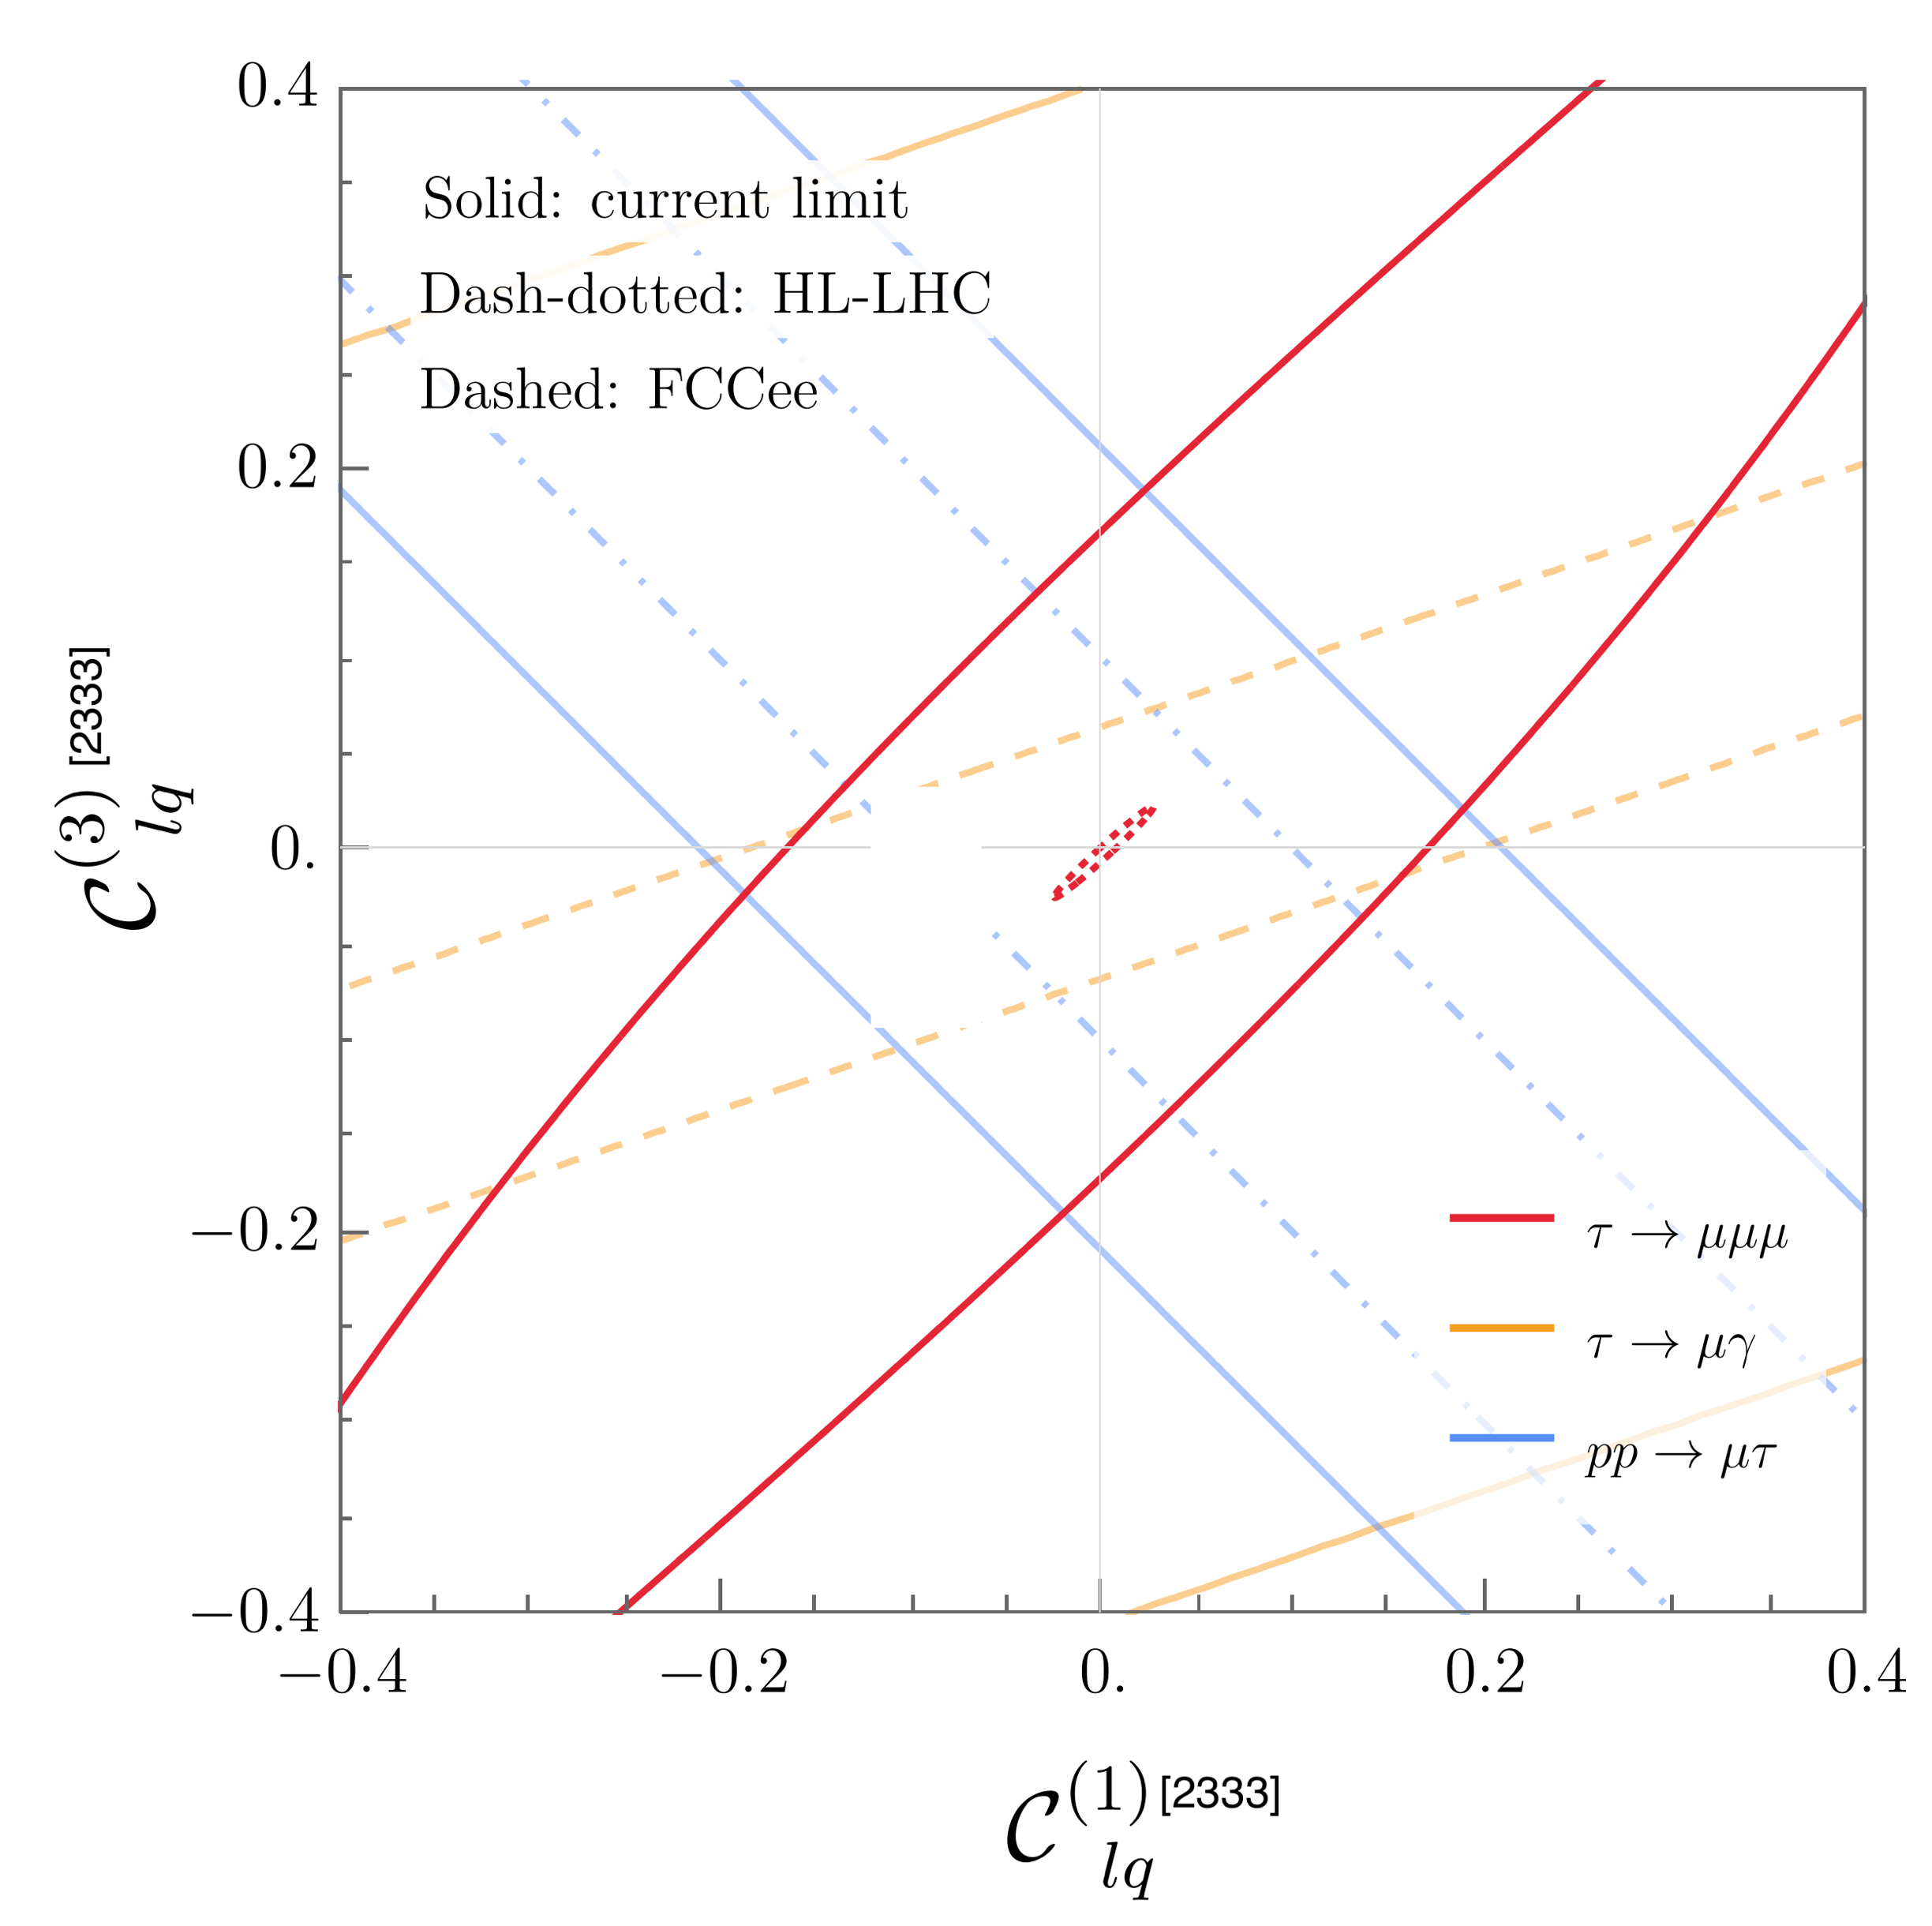
\includegraphics[width=0.4\textwidth]{Physics/PhysicsCase/Figs/Tau_LFV.png}
\caption{Left: Direct measurements of $\mathcal{B}(\PGt \to \ell \PGn \PAGn)$ branching fraction and \PGt lifetime (ellipse) 
compared to the SM prediction (band); 
the width of the SM band is determined by the \PGt mass uncertainty. From Ref.~\cite{Lusiani:2024tau}.
Right: FCC-ee impact in constraining, at 95\%~CL, 
the coefficients of representative dimension-six LFV operators normalised to the 1\,TeV scale.
Adapted from Ref.~\cite{Plakias:2023esq}, scaled to the baseline FCC-ee luminosities.
\label{fig:tauLFU}}
\end{figure}

\subsubsection{Lepton flavour violating \texorpdfstring{\PGt}{tau} decays} 

Searches for LFV \PGt decays are null tests of the SM and, thus, are pristine targets for indirect NP searches. 
A variety of explicit models, predicting rates not far from  current exclusion bounds, 
exist in the literature~\cite{Cornella:2021sby, Ardu:2021koz, Plakias:2023esq}, 
and FCC-ee will offer the ultimate experimental sensitivity on virtually 
all \PGt LFV decay modes~\cite{Li:2018cod, Dam:2018rfz, Banerjee:2022xuw}.
For example, the 90\%~CL projected limit on $\mathcal{B}(\PGt \to 3 \PGm)$ 
would be $2 \times 10^{-11}$ in absence of signal~\cite{Lusiani:2024tau}, 
which is three orders of magnitude below the current limit ($2.1 \times 10^{-8}$~\cite{ParticleDataGroup:2024cfk}) 
and more than an order of magnitude better than the final Belle~II projection (with 50\,ab$^{-1}$). 
The impact of such bounds is illustrated in the right panel of Fig.~\ref{fig:tauLFU}.
    
\subsubsection{Rare \texorpdfstring{\PQb}{b}-hadron decays with \texorpdfstring{$\PGtp\PGtm$}{taubar tau} pairs in the final state} 

In all these processes, there is an unexplored gap of about three orders of magnitude 
between SM predictions~\cite{Bobeth:2013uxa, Bouchard:2013mia, Kamenik:2017ghi} 
and experimental data~\cite{BaBar:2016wgb,LHCb:2017myy} 
--- a gap that represents a wide unexplored parameter range 
of motivated new-physics models~\cite{Buttazzo:2017ixm,Capdevila:2017iqn,Bauer:2021mvw}. 
At the SM predicted rates, FCC-ee is expected to be able to measure these decays, 
in particular $\PBz \to \PK^{*0} \PGtp \PGtm$~\cite{Li:2020bvr, miralles_2024_9t6w9-mmd12}.

\subsubsection{Charged-current \texorpdfstring{\PQb}{b}-hadron decays with a \texorpdfstring{$\tau\nu$}{tau nu} pair in the final state} 

The persisting anomalies in exclusive $\PQb \to \PQc\PGt\PGn$ decays~\cite{HFLAV:2022esi} 
give a strong phenomenological motivation for deeper studies 
of these processes~\cite{Fajfer:2012jt,Alonso:2015sja,Bernlochner:2017jka, Ho:2022ipo}.
A unique opportunity offered by the FCC-ee programme would be the experimental access 
to the clean inclusive~\cite{Ligeti:2014kia,Ligeti:2021six} 
and leptonic~\cite{Amhis:2021cfy, Zheng:2020ult} modes, 
as well as the suppressed $\PQb \to \PQu$ transitions~\cite{Aebischer:2022oqe,Fuentes-Martin:2019mun}.  
For example, the measurement of the \mbox{$\PB \to \PGt \PGn$} branching ratio at FCC-ee~\cite{Zuo:2023dzn} 
is expected to yield ultimate precision on $|V_{\PQu\PQb}|$, 
with an estimated relative uncertainty of only 1\%, 
which is a factor of three below current best estimates~\cite{HFLAV:2022esi} 
and more than a factor of two below the projected precision from the $\PB \to \PGt \PGn$ measurement at Belle~II~\cite{Belle-II:2018jsg}.

\subsubsection{Rare \texorpdfstring{\PQb}{b}- and \texorpdfstring{\PQc}{c}-hadron decays to di-neutrino final states} 

A recent sensitivity study~\cite{Amhis:2023mpj} has shown that the branching ratios of the rare 
$\PBz \to \PK^{*0} \PGn\PAGn$, 
$\PBz \to \PKzS \PGn\PAGn$, 
$\PBs \to \PKzS \PGn\PAGn$, and 
$\PGLzb \to \PGL \PGn\PAGn$ decays 
could be determined at FCC-ee with precisions of 0.53\%, 1.20\%, 3.37\%, and 9.86\%, respectively, 
relative to the current SM estimates~\cite{Bause:2021cna}. 
In particular, the precision on the \PB decay modes would exceed that expected from Belle~II by an order of magnitude, 
while the \PBs and \PGLzb modes, accessible at FCC-ee, 
would uniquely constrain possible new physics in $\PQb \to \PQs \PGn\PAGn$ transitions, 
as illustrated in the left panel of Fig.~\ref{fig:bsnunu}.

\begin{figure}[ht]
\centering 
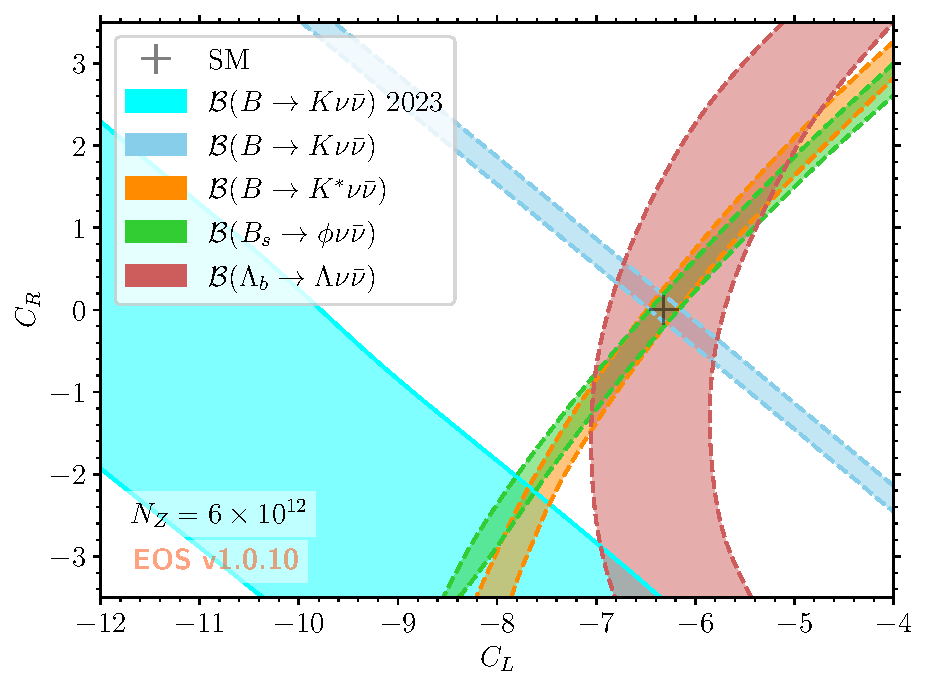
\includegraphics[width=0.5\textwidth]{Physics/PhysicsCase/Figs/WET_fit.pdf}
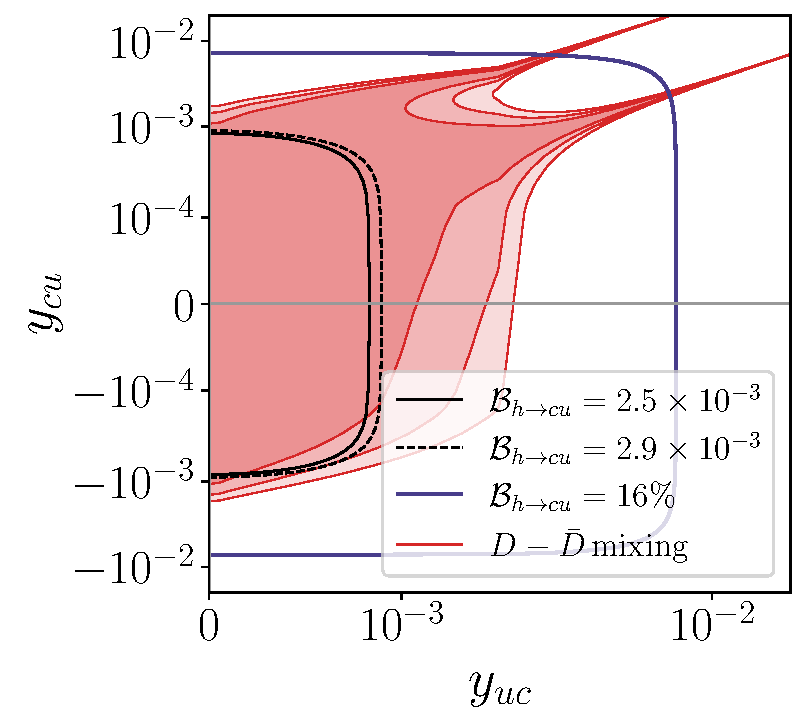
\includegraphics[width=0.4\textwidth]{Physics/PhysicsCase/Figs/cu_plot_limits.pdf}
\caption{Left: Comparison between the current constraint 
on the relevant effective $\PQb \to \PQs \PGn\PAGn$ transition operator coefficients ($C_{L,R}$) 
due to existing measurements~\cite{Belle-II:2023esi} (cyan band) 
and the (systematic-error dominated) sensitivities predicted at FCC-ee (blue, orange, green, and red bands)~\cite{Amhis:2023mpj}. 
The projected regions denote the 68\% probability of the marginal posterior density, assuming that all observables are SM-like. 
The Wilson coefficients are normalised to an effective scale of 6.5\,TeV, 
up to the CKM factors $V_{\PQt\PQs} \times V_{\PQt\PQb}$~\cite{Amhis:2023mpj}.
Right: Current (from \PD-\PAD mixing) and projected (from FCC-ee searches for $\mathrm{h} \to \PQc \PQu$) 
limits on effective charm-up flavour-changing Yukawa couplings of the Higgs boson~\cite{Kamenik:2023hvi}. 
The 68\%, 95\%, and 99.7\%~CL regions allowed by \PD-\PAD mixing data are depicted from darker to lighter red.}
\label{fig:bsnunu}
\end{figure}

Furthermore, the large number of expected events could uniquely allow more detailed differential studies of decay kinematics 
beyond simple branching ratios. 
Such measurements can also efficiently probe possible BSM effects 
in terms of the production of light invisible particles in the final state, 
mimicking the missing energy signature of the neutrino pair in the SM~\cite{Bolton:2024egx}.
 
In the charm sector, processes mediated by the $\PQc \to \PQu \PGn\PAGn$ transition are unique probes of up-quark FCNCs 
because they do not receive long-distance QCD contributions plaguing related non-leptonic or rare semileptonic decays~\cite{Artuso:2008vf}. 
In addition, SM gauge invariance and approximate $U(2)$ flavour symmetry 
relate these quark-flavour-changing processes to rare (semi)leptonic kaon decays~\cite{Bause:2020auq, Bause:2020xzj, Fajfer:2023nmz}, 
thus making them crucial in (over)constraining BSM effects in FCNCs involving the first two quark generations.  
Finally, the light dark sector coupling to $\PQc \to \PQu$ quark currents~\cite{Kamenik:2011vy, Li:2023sjf} 
can be probed with the missing energy signature, 
similar to the $\PQb \to \PQs$ transition in the \PQb-quark sector. 
Currently, the only experiment probing these processes is BES~III, which set the first upper limit, 
$\mathcal B(\PDz \to \PGpz \PGn \PAGn) < 2.1 \times 10^{-4}$ at 90\%~CL~\cite{BESIII:2021slf}. 
Based on na{\"\i}ve luminosity scaling, 
this bound could be improved by more than two orders of magnitude at FCC-ee 
and would thus make it relevant to probe flavour $U(2)$ invariant BSM scenarios~\cite{Fajfer:2023nmz}.  

\subsubsection{Rare decays and CPV studies with neutrals}

The discovery of CP violation in singly Cabibbo-suppressed \PD decays by LHCb~\cite{LHCb:2019hro} 
opened a new and largely unexplored venue for CPV studies. 
One of the outstanding puzzles is to understand whether the observed size of CPV 
is due to SM effects enhanced by long distance QCD dynamics, 
or a possible signal of NP~\cite{Chala:2019fdb, Dery:2019ysp}. 
Recent phenomenological studies using isospin~\cite{Grossman:2012eb, Gavrilova:2023fzy} 
and $U$-spin~\cite{Grossman:2019xcj, Bause:2022jes} expansions 
have shown that the measurements of decay rates and CP asymmetries in related \PD and \PDs decays 
to final states involving \PGpz and \PKzS, 
which are not possible at LHCb but would be accessible at FCC-ee, could yield a definite answer.
Important representative studies also include CP violation in 
radiative singly Cabibbo suppressed modes~\cite{Isidori:2012yx, Gisbert:2020vjx, Adolph:2022ujd}
and the doubly-radiative decay $\PDz \to \PGg \PGg$ 
required for the SM prediction of $\PDz \to \PGmp \PGmm$~\cite{Burdman:2001tf}.  
    
In the \PB sector, rates and CP asymmetries of rare radiative decays, mediated by the $\PQb \to \PQs \PGg$ transition, 
such as $\PB \to \PK^* \PGg$ and $\PB \to \mathrm{X_s} \PGg$, 
are most-sensitive probes of quark flavour violating dipole transitions~\cite{Fajfer:2023gie} 
in both minimally violating and $U(2)$ flavour models;
they are also crucial probes of flavour dynamics in composite Higgs models~\cite{Glioti:2024hye}. 
Improvements in the understanding of these decays~\cite{Benzke:2010tq, Paul:2016urs} 
are needed to fully leverage the prospective sizes of the FCC-ee event samples~\cite{BKgamma}. 
Recent steps in this direction are documented in Refs.~\cite{Gunawardana:2019gep,Misiak:2020vlo}.
Finally, time-dependent studies of rare decays, 
such as $\PBs \to \PGmp \PGmm$~\cite{Buras:2013uqa, Fleischer:2017yox}, 
$\PB \to \PKS \ell^+ \ell^-$~\cite{Descotes-Genon:2020tnz, Fleischer:2022klb}, $B_s \to \phi \mu^+\mu^-$~\cite{Kwok2024},
and $\PB \to \PKS \PGn\PAGn$~\cite{Descotes-Genon:2022gcp}, 
offer novel and complementary probes of CP violation beyond the SM, 
some only accessible at FCC-ee.     

\subsubsection{On-shell \texorpdfstring{\PZ}{Z}, \texorpdfstring{\PW}{W}, and Higgs flavour-changing decays}

Flavour-changing decays offer unique novel probes of SM and BSM flavour dynamics 
and can be searched for in inclusive final states 
(profiting from the unparalleled jet-flavour tagging capabilities of the detectors) 
or in exclusive final states~\cite{dEnterria:2023wjq}. 
In particular, $\PW \to \PQb \PQc$ decays could yield the ultimate precision on $|V_{\PQc\PQb}|$, 
with a relative uncertainty well below 1\%~\cite{WWVcb,WWVcb2}. 
Similarly, rare four-body \PZ decays could uniquely determine individual flavour neutrino couplings~\cite{Durieux:2015hsi}.
Furthermore, lepton-flavour-violating Higgs and \PZ decays involving \PGt leptons in the final state 
would improve existing LEP and LHC constraints by orders of magnitude~\cite{Abada:2014cca, Qin:2017aju, Dam:2021ibi}. 
Finally, FCC-ee could also directly probe FCNC decays of \PZ and Higgs bosons~\cite{Kamenik:2023hvi}, 
possibly even reaching SM expectations for the former (in the case of $\PZ \to \PQb\PQs$) 
and surpassing indirect constraints from neutral meson oscillation measurements for the latter, 
as shown in the right panel of Fig.~\ref{fig:bsnunu}. 
Such direct measurements are also particularly important to lift degeneracies in BSM fits 
and disentangle possible UV sources of low energy FCNC effects~\cite{Crivellin:2022rhw}. 

\subsubsection{Combined studies and synergy between the flavour and EW programmes}
\label{sect:flavour-synergy}

Besides the interest of the specific observables illustrated above, 
probably the most interesting aspect of the FCC flavour programme lies 
in the possibility of combining several precision flavour-violating and flavour-conserving measurements. 
This combination offers a unique opportunity to characterise a possible NP signal, 
when it emerges, as illustrated in the next two paragraphs. 

\subsubsubsection{New-physics in \texorpdfstring{\PB-\PAB}{B-Bbar} mixing}

Measurements of $\phi_{\PQs}$ from $\PBs \to \PJGy\, \PGf$ and $\PBs \to \PGf \PGf$ at FCC-ee 
could challenge present theory uncertainties~\cite{Aleksan:2022mtk, Gerlach:2022hoj}. 
Similarly, the full exploitation of experimental precision on $\Delta m_{\PQs}$ 
will hinge upon the determination of $|V_{\PQc\PQb}|$ at or below the sub-per-cent level~\cite{Lenz:2019lvd, Charles:2020dfl} 
from either (inclusive) semileptonic \PB decays, 
leptonic \PBc decays~\cite{Amhis:2021cfy, Zheng:2020ult}, 
or on-shell $\PWp \to \PAQb \PQc$ decays~\cite{WWVcb, WWVcb2}. 
As an illustration of the increased sensitivity achieved by combining all these measurements, 
the NP reach in the $\PB_{\PQs,\PQd}$ mixing amplitudes is shown in Fig.~\ref{fig:dF2}.
Mainly due to the increased precision on $|V_{\PQc\PQb}|$, 
the effective NP scale sensitivity would increase by a factor of three compared to current measurements 
and by a factor of 1.5 compared to the ultimate precision expected at Belle~II.   
It is worth stressing that FCC-ee will also deliver the ultimate determination of the CKM-matrix $\gamma$ angle 
from $\PB \to \PD \PK$ decays~\cite{Brod:2013sga}, 
allowing a per-mil test of CKM unitarity in the $\PQb \to \PQs$ triangle~\cite{Aleksan:2021fbx, Aleksan:2021gii, Aleksan:2024jwm} 
(one order of magnitude better than the current sensitivity), 
as well as the possibility to test the SM predictions for mixing-induced semileptonic CP asymmetries 
in both $\PBd$ and $\PBs$ decays~\cite{Artuso:2015swg,Jubb:2016mvq, Lenz:2020efu}.

\begin{figure}[ht]
\centering
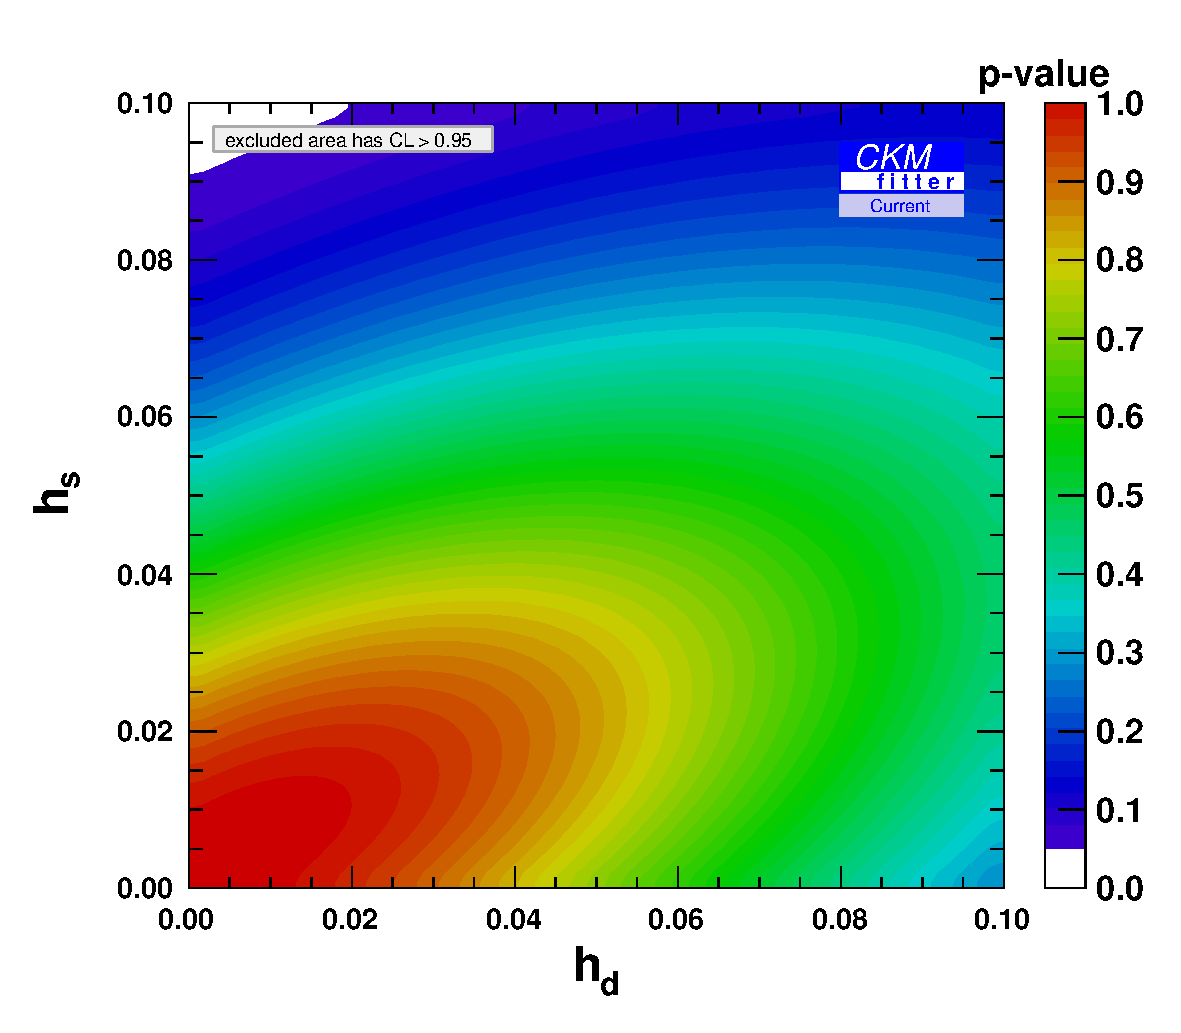
\includegraphics[width=0.32\textwidth]{Physics/PhysicsCase/Figs/hdhs_Phase0_zoom.pdf}
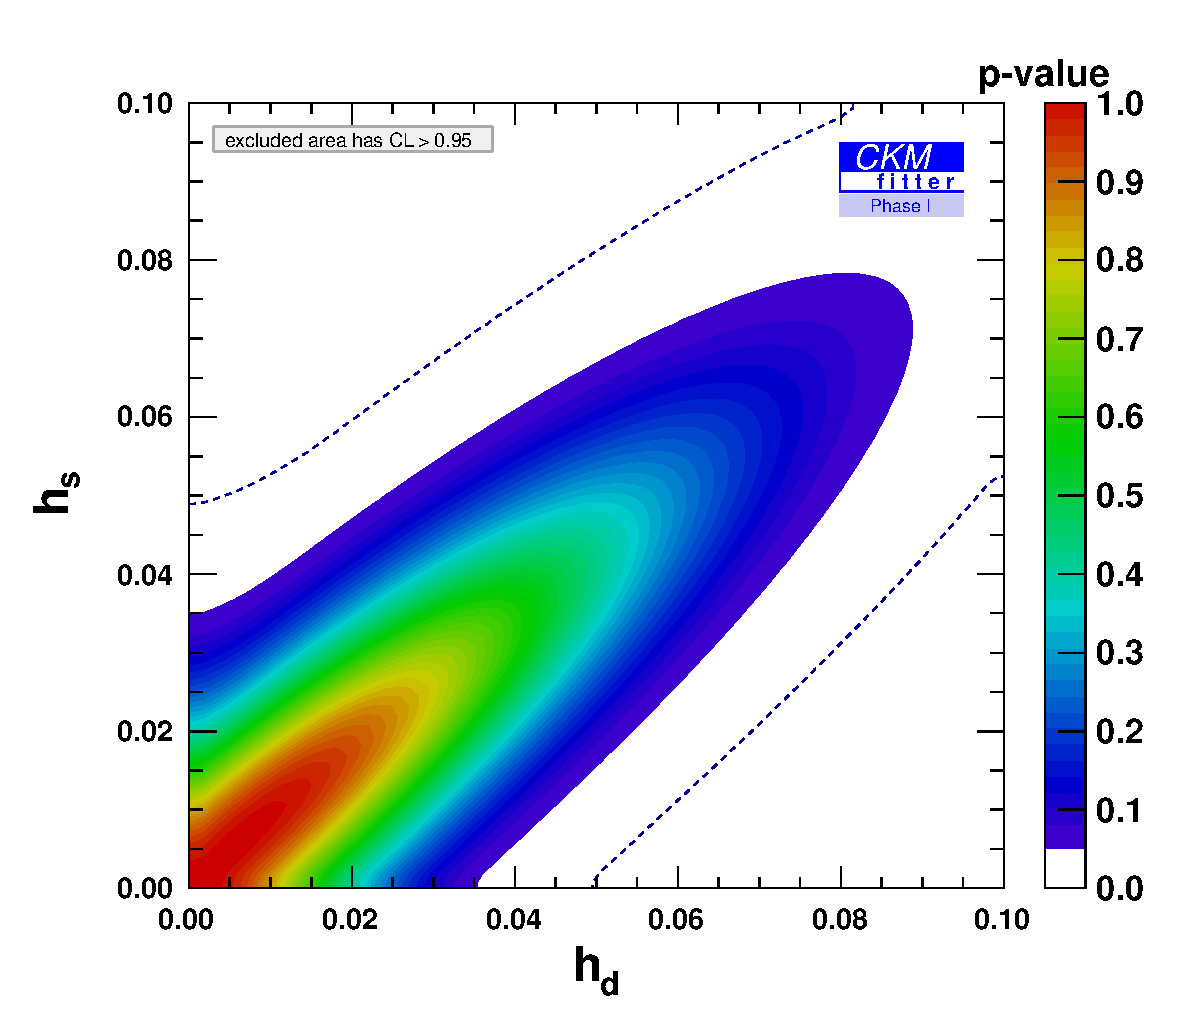
\includegraphics[width=0.32\textwidth]{Physics/PhysicsCase/Figs/hdhs_PhaseI_zoom.pdf}
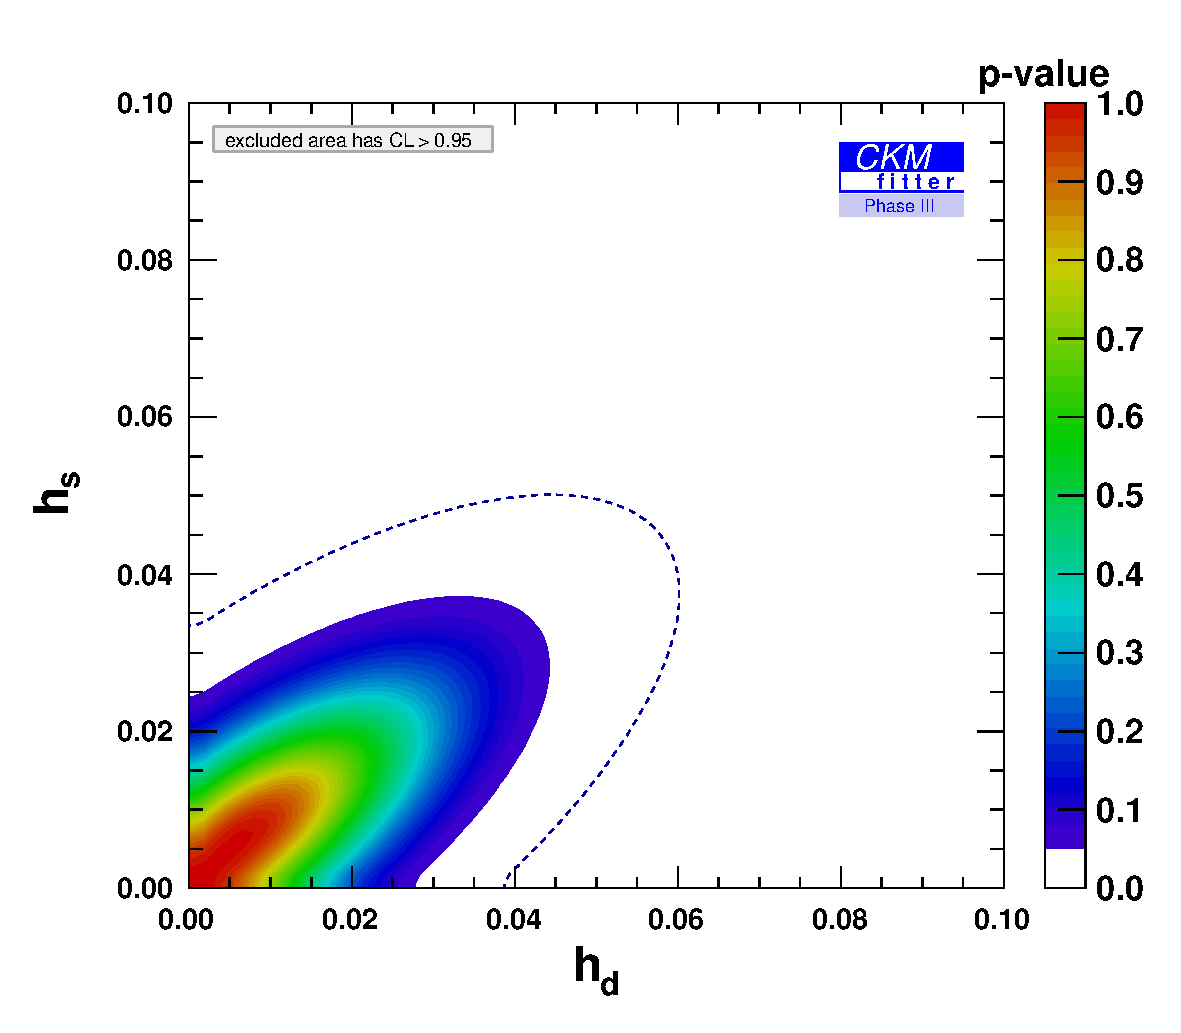
\includegraphics[width=0.32\textwidth]{Physics/PhysicsCase/Figs/hdhs_PhaseIII_zoom.pdf}
\caption{Sensitivities to relative BSM amplitudes ($h_{\PQd}$ and $h_{\PQs}$) in \PBd and \PBs mixings:
current values (left), 
LHCb (50\,fb$^{-1}$) and Belle~II (50\,fb$^{-1}$) projections (centre),
and FCC-ee projections (right).
From Ref.~\cite{Charles:2020dfl}. 
A limiting factor of the FCC-ee sensitivity is the uncertainty on $V_{\PQc\PQb}$, 
expected to be reduced with the $\PW\PW$ threshold run and from improved flavour-tagging algorithms.
\label{fig:dF2}}
\end{figure}

\subsubsubsection{Synergy with the EW programme}

A particularly interesting synergy emerges when combining flavour-violating and EW observables. 
The discovery potential offered by this combination in a variety of NP models 
has only recently begun to be explored~\cite{Garosi:2023yxg, Allwicher:2023shc, Grunwald:2023nli}.
An illustration of this potential is presented in Fig.~\ref{fig:FlavEWFCC} 
in the context of models describing generic NP coupled mainly to the third generation, 
as defined in Ref.~\cite{Allwicher:2023shc}. 

\begin{figure}[ht]
\centering 
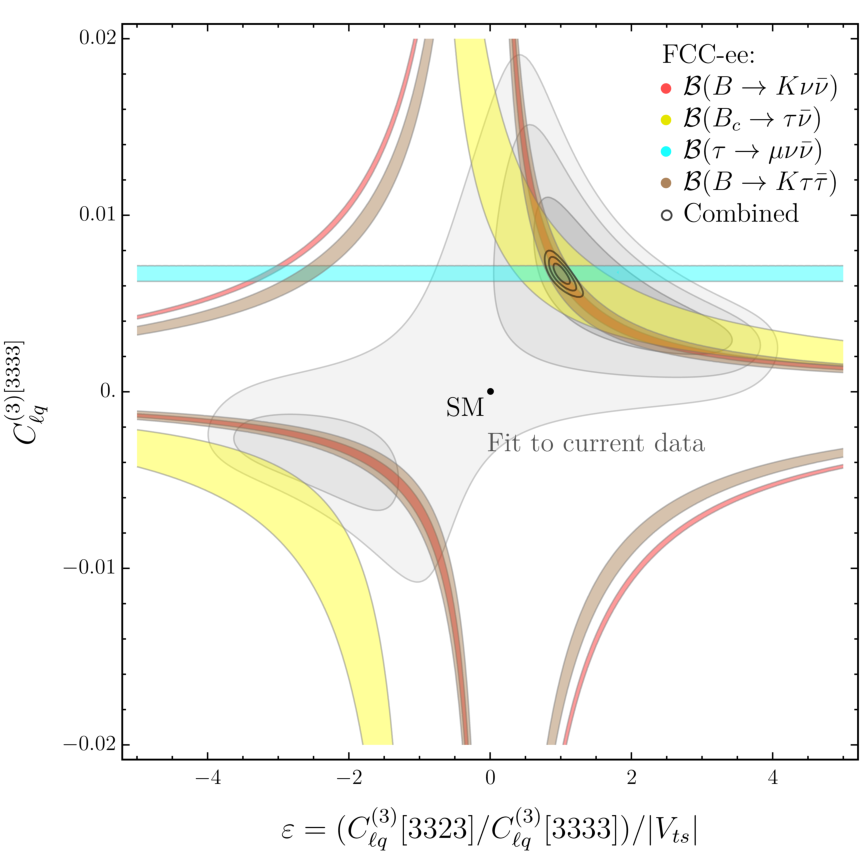
\includegraphics[width=0.42\textwidth]{Physics/PhysicsCase/Figs/Clq3vsepsilon_FSR.pdf} 
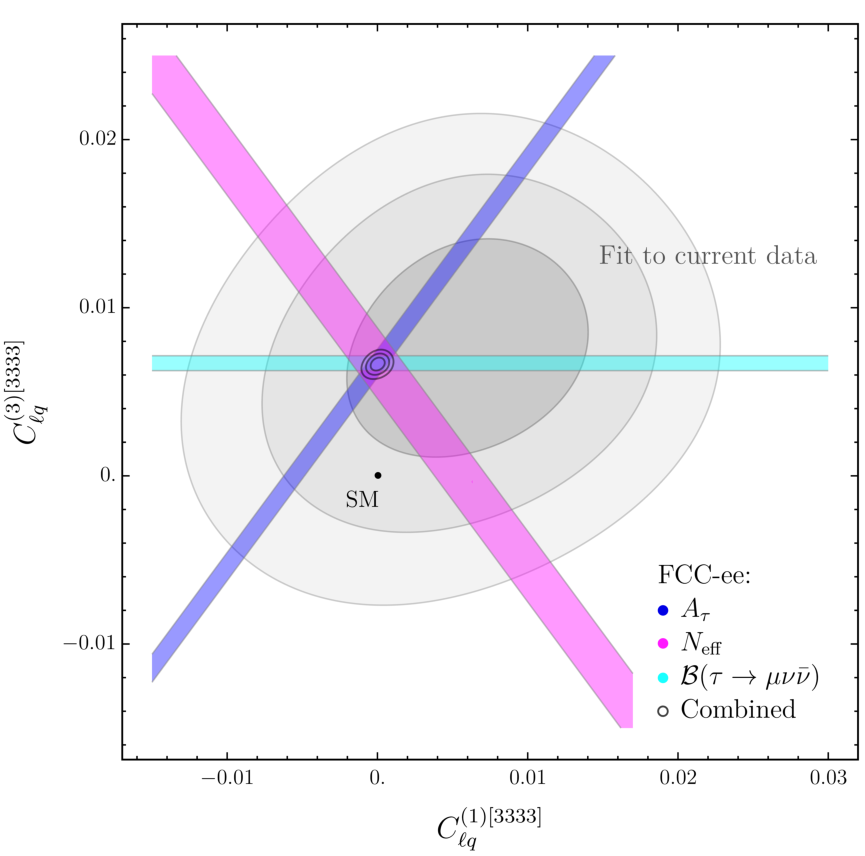
\includegraphics[width=0.42\textwidth]{Physics/PhysicsCase/Figs/Clq3vsClq1_FSR.pdf}
\caption{Constraints on semileptonic effective operators describing new physics coupled mainly to the third generation 
with minimal $U(2)$ breaking~\cite{Allwicher:2023shc}.
The grey regions show the result of the current fit (68\%, 95\%, and 98\% CL), 
including flavour, electroweak, and Drell--Yan data 
(the slight tension with the SM is driven by $\PQb \to \PQc \PGt \PAGn$ data).
The small ellipses are the result of an hypothetical fit 
with FCC-ee projected uncertainties on flavour and electroweak observables, 
assuming a signal compatible with current data.
The coloured bands are the individual constraints of the observables in this scenario.
The FCC constraints follow from the projections of a precision of 3\%, 1.6\%, 0.01\%, and 20\% 
on the $\mathcal{B} (\PB \to \PK \PGn\PAGn)$, 
$\mathcal{B}(\PBc \to \PGt \PAGn)$, 
$\mathcal{B}(\PGt \to \PGm \PGn\PAGn)$, 
and $\mathcal{B}(\PB \to \PK \PGtp\PGtm)$ values, respectively. 
From Ref.~\cite{Allwicher:2025new}.}
\label{fig:FlavEWFCC}
\end{figure}   

As can be seen in this case, different observables probe the same parameter space in different directions, 
and their combination is essential to fully characterise the hypothetical NP framework, 
with, in particular, the synergy between rare \PB decays, rare \PGt decays, 
and the flavour-conserving effective couplings of the \PZ boson. 

\subsection{FCC-hh specificities compared to high-energy lepton colliders}
\label{sec:PhysicsCaseHHvsHEL}

With operation expected to start in the mid-2040's, 
the guaranteed deliverables and primary targets of FCC-ee are 
the precise and model-independent measurement of a broad range of key couplings of the Higgs boson, 
a fifty- to thousand-fold improvement in the precision of EW parameters, 
and a precise determination of the top quark mass and EW couplings.  
A 3\,TeV muon collider has also been proposed, for a timescale similar to that of FCC-ee~\cite{Black:2022cth}.
The best-measured Higgs couplings, $\kappa_{\PZ}$ and $\kappa_{\PW}$, 
will be measured at FCC-ee with expected uncertainties of 0.11\% and 0.29\%, respectively (Table~\ref{tab:HiggsKappa3}),  
much better than the 0.9\% and 0.4\% uncertainties foreseen at a 3\,TeV muon collider~\cite{MuonCollider:2022xlm}.  
This observation, combined with the \mbox{Tera-\PZ} programme and the $10^6$ top pairs at FCC-ee, 
as compared to orders of magnitude fewer at a 3\,TeV muon collider, 
renders FCC-ee the obvious priority for Higgs, electroweak, top, and flavour physics to follow HL-LHC.  
This section considers the question of what should follow FCC-ee as a high-energy exploration facility, 
comparing and contrasting frontier ($\gtrsim 10$'s\,TeV) lepton collider options with FCC-hh.

\subsubsection{Generalities}

Exploration in particle physics cannot be quantified by the volume of parameter space explored, nor by the scale of the energy reached.  
Indeed, LHC has shown that the microscopic world that can be explored by hadron colliders 
is so multidimensional and rich that no metric can fairly convey the depth 
with which the laws of nature are explored by colliding protons.  
Yet, looking to future high-energy facilities, this is precisely what must be attempted.

The core attribute of a proton collider is that it does not simply collide a single particle and an antiparticle but, instead, 
collides anything found in the proton; 
any of the lightest five quarks and antiquarks, the gluons, the photon, and the EW gauge bosons. 
Thus, a proton collider has many particle colliders in one, operating at the highest plausibly achievable energies, 
with an array of production channels for discovery and exploration that is factorially greater 
than what can be achieved by colliding single fundamental particles 
--- besides the additional possibility of colliding heavy ion in the same machine.  
The price to be paid for this great leap in exploratory power is the inherent messiness of the final state from colliding composite objects.  
However, this challenge has been amply met at LHC and there is no reason to expect something else at a future proton collider.

Were some hints for new physics at high energies to appear in the Run~3 of LHC or at HL-LHC, 
it is highly unlikely that identification of the microscopic production channel from which it emerged would be possible at HL-LHC. 
Depending on the new physics at stake, 
the FCC-ee precision data may exhibit interesting patterns of deviations that 
would refine the interpretation of these hints and give precious information about their quantum origin. 
At high energy, however, the only way to guarantee further exploration and characterisation of whatever may arise at LHC 
would be to collide protons once again, with greater energy and larger collected event samples, 
possibly activating additional production channels and dynamical regimes: 
this is the only way to cover all possible production channels.

Also, it is worth noting that the discovery of the Higgs boson opened windows beyond the gauge paradigm 
to a new class of fundamental forces and to the flavour puzzle.  
Modern particle physics exploration should be equipped to navigate this new world.  
The case, for example, of a new neutral scalar coupled to fermions with a strength proportional to their mass is enlightening. 
Clearly, the third generation quarks provide the most immediate access to such a sector, 
whether through production by $\bbbar$ annihilation or through gluon fusion via a top quark loop.  
This is, after all, how the Higgs boson was discovered.  
Such scenarios should not be blind spots for any future facility and, indeed, 
a future proton collider would provide excellent discovery opportunities for states that do not carry electroweak charges.
%
Some more concrete, yet still general, future discovery possibilities are considered below.

\subsubsection{Resonance searches}

A key exploratory task for any high-energy exploration facility is to search thoroughly for new high-mass resonances. 
There are two complementary approaches to probe the existence of high-mass states: 
the direct search for a mass peak 
and the indirect evidence emerging from deviations in precise measurements of processes accurately predicted within the SM. 
The indirect approach extends the sensitivity of a collider well beyond its kinematic reach. 
As clearly shown by LEP2, 
the superior precision of a lepton collider can therefore 
match the sensitivity of direct searches at hadron colliders of much higher centre-of-mass energies. 
The limitation of the indirect approach, however, 
is that the interpretation of such deviations is very much dependent on model assumptions. 
For example, the new state masses can vary significantly as a function of the assumptions on their couplings. 
Outside a well-defined theoretical BSM framework, for which there is no compelling prejudice today, 
this ambiguity significantly limits the ability to point to new measurements that would clarify the source of new physics. 
Direct search, when possible, therefore provides a preferable (yet synergistic) approach, 
when the indirect and direct sensitivity of lepton and hadron colliders are numerically comparable. 

For this reason, the focus here is on the comparison of FCC-hh and high-energy lepton colliders to the case of direct detection. 
Present theory priors do not favour any particular possibility, 
thus the breadth of couplings that can be explored is a paramount consideration in planning for the future.
For this purpose, a proton collider has a further unique virtue, sampling a wide array of initial states, 
from gluons to photons or EW gauge bosons and quarks of a variety of flavours, 
and from neutral initial states to charged or even coloured, 
any of which could lead to the formation of a new resonance.
For example, 15 $\qqbar^{(')}$ initial states can create exotic bosonic resonances, 
both in flavour-conserving and flavour-violating channels. 
Besides, 20 $\mathrm{V}+\PQq$ initial states could create excited quark states (with $\mathrm{V} = \PGg$, \Pg), 
or new heavy quarks through charged ($\mathrm{V} = \PW$) or neutral ($\mathrm{V} = \PZ$) current transitions. 
Furthermore,
8~$\mathrm{V}\mathrm{V}^\prime$ initial states can give rise to EW resonances 
or axion-like particles ($\mathrm{V},\mathrm{V}^\prime = \PGg, \PW, \PZ$), or to $\Pg\Pg$ resonances.

Another key component of exploration combines breadth with energy.  
As a figure of merit, proton colliders can be compared with lepton colliders to assess their relative reach in energy for resonances.  
Following Ref.~\cite{AlAli:2021let}, an optimistic scenario is considered, 
where a new high-energy resonance (serendipitously) resides at the kinematic limit of a lepton collider 
and can be produced by that initial 
state\,\footnote{For lower masses, radiative-return production would be required to enable discovery.}. 
The energy of proton collisions that would be necessary to produce the same number of resonant events, 
given the same integrated luminosity, is a natural figure of merit here. 

\begin{figure}[ht]
\centering
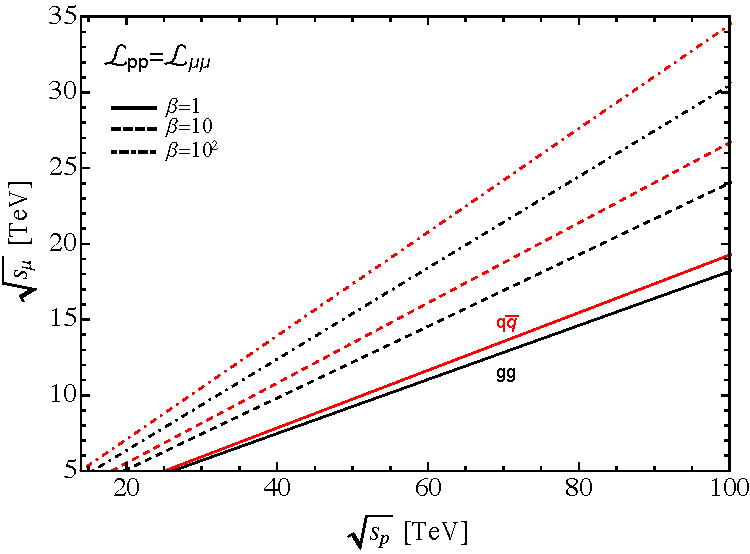
\includegraphics[width=0.55\textwidth]{PhysicsCase/Figs/ResonanceComp.pdf} 
\caption{Energies of equivalent event numbers, 
assuming equal integrated luminosities, 
between a high-energy muon collider and a proton collider;
$\beta=1$ corresponds to the same partonic cross section between muons and proton partons while
larger values of $\beta$ correspond to enhanced partonic cross sections for quarks and gluons, 
as would be the case for resonances coupled primarily through QCD.  
Note that $\beta<1$ would require muons to be more strongly coupled to new resonances than quarks, 
requiring muon flavour to play a role.}
\label{fig:resonancecomp}
\end{figure}

The resulting equivalent CM energy is shown in Fig.~\ref{fig:resonancecomp}, 
under the assumption that the parton-level production cross sections are a factor $\beta = 1$, 10, 100 larger than 
the lepton-collider production cross section on resonance for $\qqbar$ and $\Pg\Pg$ initial states.  
It is noteworthy that, 
even under the significant assumption that the production cross section via leptons matches that of quarks or gluons ($\beta = 1$),  
a 100\,TeV proton collider significantly exceeds, for such a resonance, the reach of a 10\,TeV lepton collider.  
For larger parton production cross sections relative to leptons, 
the gap in coverage between the two classes of facilities further increases.  
Such a comparison, however, also conceals the richness of the physics programme for such $>10$\,TeV resonances at a proton collider.

To go further, the direct discovery prospects for narrow resonances of mass $M_\mathrm{R} > 10$\,TeV, 
which would be inaccessible to a 10\,TeV muon collider, is investigated.  
In the narrow width approximation, at a proton collider operating at proton CM energy $\sqrt{s}$, 
the production cross section for a resonance R of spin $S$ coupled to the initial state partons `yy' 
and decaying into the final state `xx' is
\begin{equation}
\sigma = r \frac{C_{\rm yy}}{s} \, ,
\end{equation}
where, for gluons and quarks, the factor $C_{\rm yy}$ is related to the parton luminosity as
\begin{equation}
C_{\Pg\Pg} =\frac{\pi^2}{8} \int_\tau^1 \frac{dx}{x} \, f_{\Pg}(x) f_{\Pg}(\tau x) ~,
\quad
C_{\qqbar} =\frac{4\pi^2}{9} \int_\tau^1 \frac{dx}{x} \, 
\left[ f_{\PQq}(x) f_{\PAQq}(\tau x) + f_{\PAQq}(x) f_{\PQq}(\tau x) \right] \, ,
\label{eqCi}
\end{equation}
where $\tau = M_\mathrm{R}^2/s$ and the parton distribution functions $f_{\Pg,\PQq,\PAQq}$ 
are evaluated at $Q^2 = M_\mathrm{R}^2$. 
The parameter $r$ encodes all the model-dependent factors,
\begin{equation}
r = (2 S+1) B_{\rm yy} B_{\rm xx} \frac{\Gamma_\mathrm{R}}{M_\mathrm{R} } \, .
\label{eq:r}
\end{equation}

The width-to-mass ratio essentially encodes the microscopic coupling and hence parametrises the nature of the underlying theory.  
For these purposes, whenever $\Gamma_\mathrm{R} / M_\mathrm{R} \lesssim 0.1$, 
the theory is approximately perturbative and the resonance effectively narrow.  
In Eq.~(\ref{eq:r}), $B_{\rm yy}$ is the branching ratio into the partons whose collision produced the resonance 
and $B_{\rm xx}$ is the branching ratio into whichever final state is under consideration.  
The latter could more prosaically be a pair of SM particles or something much more exotic, such as pairs of long-lived particles.

\begin{figure}[ht]
\centering
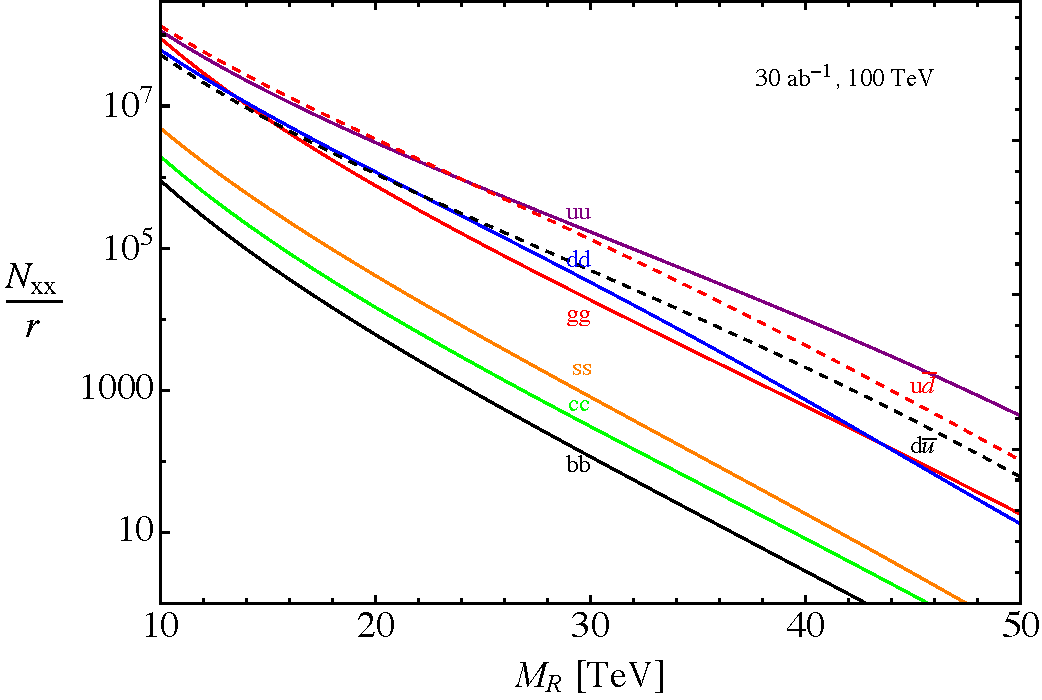
\includegraphics[width=0.55\textwidth]{PhysicsCase/Figs/Resonance.pdf} 
\caption{The number of resonance-production events at a 100\,TeV proton collider, 
relative to the model-dependent factor $r$ defined in Eq.~(\ref{eq:r}).  
A non-exhaustive variety of initial states yy is considered and the final-state decay product xx is unspecified.}
\label{fig:resonance}
\end{figure}

Figure~\ref{fig:resonance} shows the number of $\Pp\Pp \to R \to xx$ events 
for a variety of production channels at masses above 10\,TeV.  
This number of events is weighted relative to the model-dependent factor $r$.  
Simply as an illustrative example, a scalar resonance could plausibly have $r = 10^{-2}$.  
Thus, in this case, the total number of events in Fig.~\ref{fig:resonance} should be multiplied by $10^{-2}$.  
The number of events plausibly available, hence the breadth of the exploration, 
to a 100\,TeV proton collider for resonances above the 10\,TeV scale is vast.  
Smaller values of $r$ are also possible, 
with events occurring above energies of 10\,TeV even for extremely narrow resonances, down to $r \sim 10^{-8}$.  
For example, the SM Higgs boson has $r \approx 3 \times 10^{-5}$.

If the final states were rare collider objects, such as long-lived particles, 
then these many-orders of magnitude of events would be highly visible, 
offering a vast programme of not only discovery but also characterisation. 
Presumably, for such exotic decays, the discovery reach would essentially saturate kinematic and PDF limits, up to $\sim$\,50\,TeV.  
On the other hand, if the final states were not rare but visible, such as to photons or leptons, 
then such a resonance would also stand out above the background. 
This is confirmed, for example, for the Sequential Standard Model scenario reach for leptonic decays shown in Fig.~\ref{fig:schannel}, 
where the reach extends beyond 40\,TeV.  
These are the easiest discovery opportunities that would maximise the opportunities of the statistical reach of the large event samples.

Finally, even in scenarios where the final state has a significant background, 
the number of events is large enough that a discovery would still be expected.  
This point is confirmed by detailed studies for specific scenarios.  
For instance, Fig.~\ref{fig:schannel} also shows the discovery reach for a variety of $s$-channel resonances.  
Even for a dijet final state, for which there is overwhelming background, the discovery reach extends to the 40\,TeV scale.

\subsubsection{Pair production of new particles}

Figure~\ref{fig:paircomp} shows the result of a similar exercise as for the resonances, 
again following Ref.~\cite{AlAli:2021let} and assuming the same integrated luminosity for each collider, 
and wondering what energy of muon collider would produce the same number of pair-production events 
as a proton collider operating at a CM energy $\sqrt{s_{\Pp}}$.  
To do this, it is assumed that the muon collider can produce states close to threshold and, 
considering partonic cross sections
\begin{equation}
\hat{\sigma}_{\rm ij\to xx}(s_\mu) = \beta \hat{\sigma}_{\mu^+ \mu^-\to \rm xx}(s_\mu)
\end{equation}
(where $\rm ij = \Pg\Pg, \qqbar$ are the initial state partons and xx are the pair-produced new states), 
it is also assumed that the energy dependence of the cross section is inversely proportional to the partonic energy-squared.  
As before, $\beta \approx 1$ qualitatively corresponds to new states that couple equally strongly to the muons and the partons.  
Such scenarios would involve the production of purely electroweak states, or states with flavour-independent couplings. 
Instead, $\beta \approx 10$--100 corresponds to states that may also carry colour.  
Going beyond this, states that only couple to gluons or couple proportionally to fermion masses would have $\beta \gg 100$.

\begin{figure}[ht]
\centering
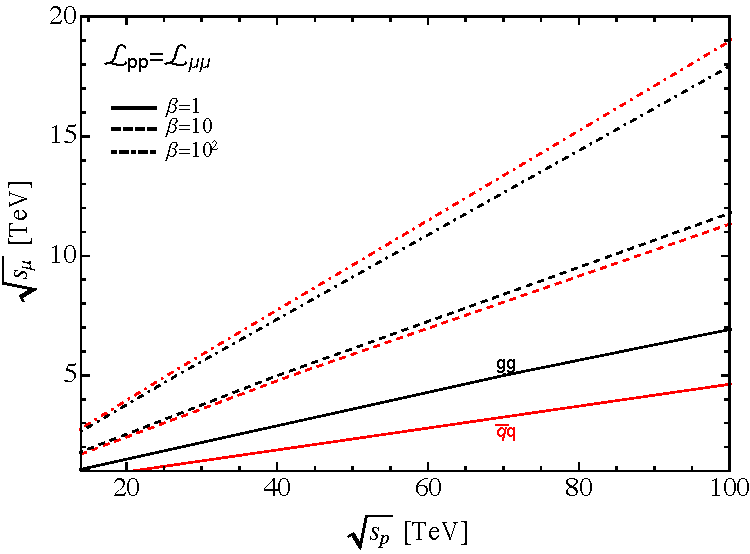
\includegraphics[width=0.55\textwidth]{PhysicsCase/Figs/PairComp.pdf} 
\caption{Same as Fig.~\ref{fig:resonancecomp}, but for pair-produced resonances.}
\label{fig:paircomp}
\end{figure}

It can be seen from Fig.~\ref{fig:paircomp} that only for the case of $\beta \approx 1$, 
hence essentially only purely EW states, 
does a 10\,TeV muon collider have an estimated reach extending beyond that of a proton collider.  
This is confirmed in the simple example of supersymmetry, 
where the estimated discovery reach for coloured particles shown in Fig.~\ref{fig:SUSY} 
for a 100\,TeV proton collider extends beyond 10\,TeV, 
hence beyond the kinematic limit of a 10\,TeV muon collider.  
For purely electroweak particles, the proton collider reach saturates at around the 5\,TeV scale, 
close to the kinematic limit of a 10\,TeV muon collider.

\begin{figure}[ht]
\centering
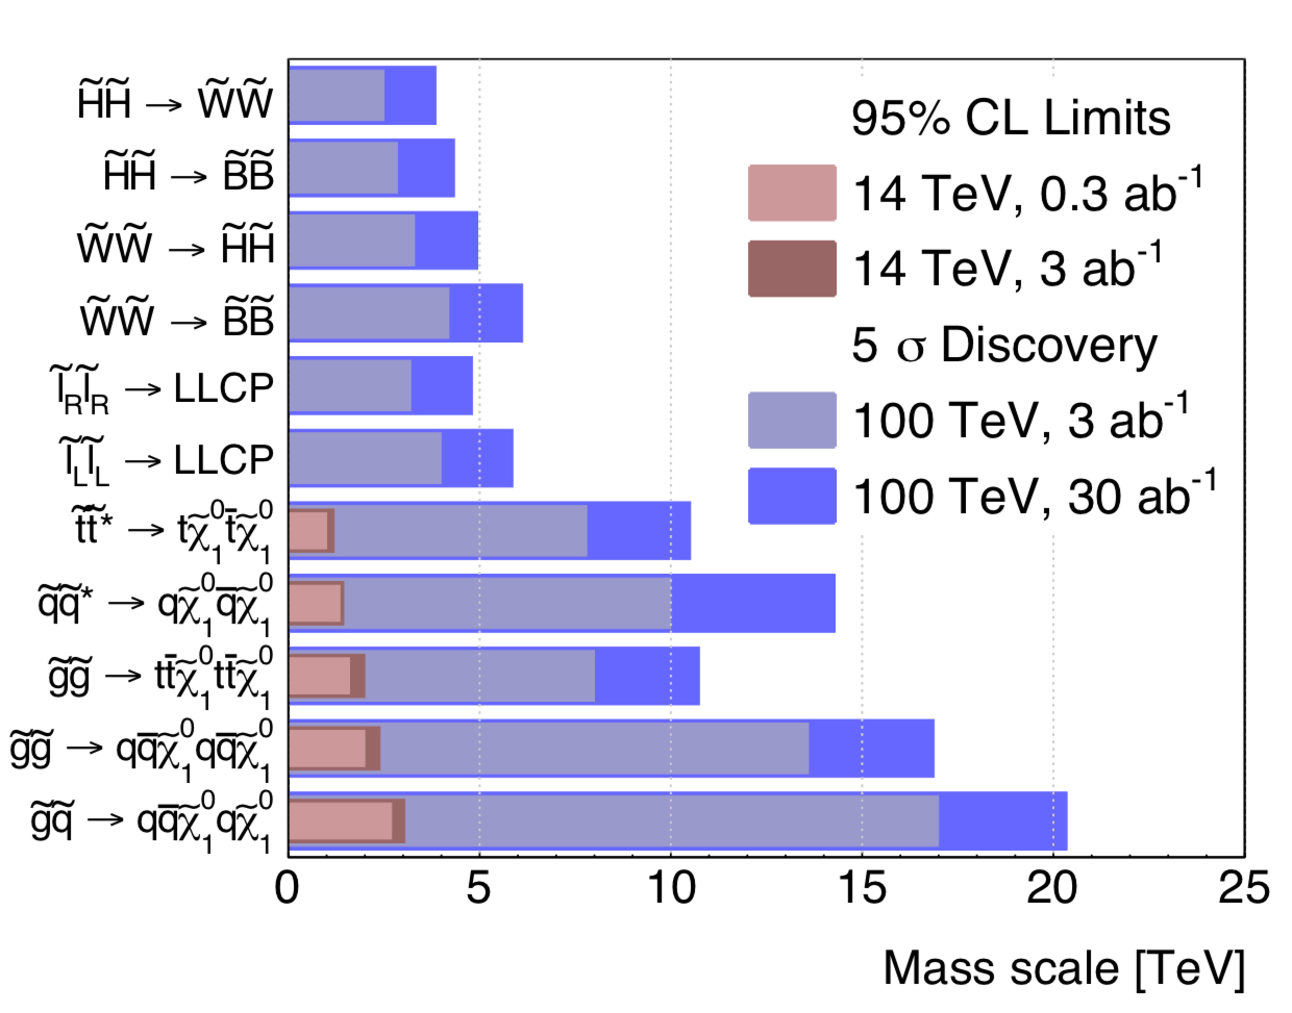
\includegraphics[width=0.55\textwidth]{PhysicsCase/Figs/SUSY.pdf}
\caption{Summary of the 5\,$\sigma$ discovery reach for different SUSY particles. 
From Ref.~\cite{Golling:2016gvc}.}
\label{fig:SUSY}
\end{figure}

This treatment has, however, been relatively na{\"\i}ve in the sense that it is essentially rooted in the gauge paradigm.  
It can instead be assumed that, at these energy scales, the new physics couples only through dimension-6 contact interaction. 
In this case, the production cross section at the partonic level scales proportional to the partonic energy-squared.  
Such a possibility is plausible if the states that connect the two sectors are heavy.

Figure~\ref{fig:paircomp6} shows the approximately equivalent colliders under this assumption, 
where the outcome is very different.  
In this case, a 100\,TeV proton collider exceeds the reach of a 10\,TeV muon collider 
even assuming comparable partonic cross sections at $s_\mu$, which may not be the case.

\begin{figure}[ht]
\centering
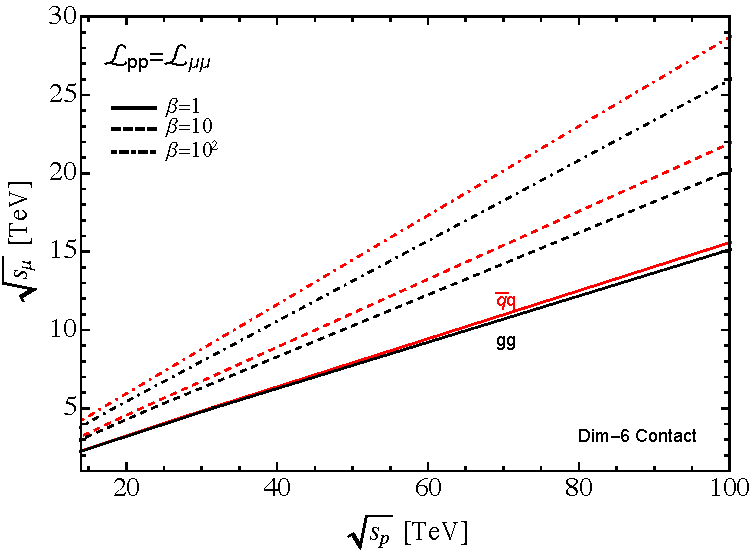
\includegraphics[width=0.55\textwidth]{PhysicsCase/Figs/PairComp6.pdf} 
\caption{Same as Fig.~\ref{fig:paircomp}, but for production through a higher-dimension operator.}
\label{fig:paircomp6}
\end{figure}

\subsection{Physics reach of alternative FCC-hh \texorpdfstring{$\sqrt{s}$}{sqrt(s)} options}
\label{sec:PhysicsCaseHHscenarios}

The reduction of the FCC tunnel length, with respect to the CDR, from 100 to 90.7\,km, 
and the range of values for the magnetic field strength of dipoles that might be ready for mass production 
on the timescale of the final definition of the FCC-hh accelerator, 
motivate a study of beam-energy scenarios alternative to the canonical $\sqrt{s}=100$\,TeV used for the CDR physics studies. 

The first results of this study are presented here, considering the cases of $\sqrt{s}=80$ and 120\,TeV. 
The former is motivated by the combined effect of a reduction in ring size and a less aggressive assumption, 
with respect to the CDR, for the strength of Nb$_3$Sn dipoles finally available (14\,T instead of 16\,T). 
The higher energy value is relevant in scenarios where high-temperature superconducting (HTS) dipoles, 
in the range of 20\,T, become available. 
A more precise and detailed assessment of the full operational scenarios, 
including therefore the estimates of the collider luminosity, is underway. 
The definition of these scenarios will be modulated by assumptions about, and interplay between, 
key elements such as overall power consumption and experimental pileup. 
The results of these more complete studies, and their impact on the physics programme, will be documented at a later stage. 

For this report, the same luminosity setting is assumed for all three energies, 80, 100, and 120\,TeV, 
namely a total of 30\,ab$^{-1}$, obtained by combining the event samples collected by two general-purpose detectors. 
The goal of the study is not to provide an accurate update of the 100\,TeV results 
but rather to focus on the loss or gain in performance for some of the key deliverables highlighted in the FCC-hh CDR, 
namely the precision study of Higgs properties, the search for high-mass resonances, 
and the potential to discover or exclude scenarios of WIMP dark matter candidates. 
The chosen energies (80 and 120\,TeV) may not match precisely the values that will emerge from the more detailed accelerator studies. 
Preliminary indications suggest, however, that they provide a 
good reference for the physics performance with dipole field strengths ranging between 12 and 20\,T. 

\subsubsection{Higgs properties}

The CDR has shown that the baseline FCC-hh programme can improve to sub-percent level the precision of Higgs decays 
such as $\PGg\PGg$, $\PZ\PGg$, and $\PGm\PGm$, 
which are too rare to be detected with that kind of precision at FCC-ee or any other proposed $\epem$ Higgs factory.
This precision is achieved by considering the ratio of Higgs bosons produced above some \pt threshold 
and decaying to a given channel, relative to those decaying to four leptons. 
For the latter, the branching ratio is expected to be known from FCC-ee with a per-mil precision. 
The ideal value of the \pt cut is defined by the optimum balance between statistical and systematic uncertainties;
typical values are in the 100 to 200\,GeV range. 
In this \pt range, the Higgs production rate is reduced (increased) by about 30\% (35\%), 
when changing $\sqrt{s}$ from 100 to 80 (120)\,TeV. 
Folding this modified statistical uncertainty with the systematic uncertainties 
leads to the projections for the measurement precision of Higgs couplings shown in Table~\ref{tab:FCChh_sce_H}.  
The 1\% statistical precision expected at 100\,TeV for the determination of 
the $\PQt\PAQt\PH\,/\,\PQt\PAQt\PZ$ production cross-section ratios is modified to 1.2\% and 0.85\%, at 80 and 120\,TeV, respectively. 

\begin{table}[ht]
\centering
\caption{Projected uncertainties of Higgs coupling measurements at FCC-hh, 
for different $\sqrt{s}$ scenarios, with an integrated luminosity of 30\,ab$^{-1}$.}
\label{tab:FCChh_sce_H}
\begin{tabular}{ l   c c   c }%| c }
\toprule
Coupling & 100 TeV & 80 TeV & 120 TeV   \\
 & CDR baseline & & \\
\midrule 
$\delta g_{\PH\PGg\PGg}/g_{\PH\PGg\PGg}~(\%)$
& 0.4 & 0.4 & 0.4 \\
$\delta g_{\PH\PGm\PGm}/g_{\PH\PGm\PGm}~(\%)$
& 0.65 & 0.7 & 0.6 \\
$\delta g_{\PH\PZ\PGg}/g_{\PH\PZ\PGg}~(\%)$
& 0.9 & 1.0 & 0.8 \\
$\delta g_{\PH\PGm\PGm}/g_{\PH\PGm\PGm}~(\%)$
& 0.65 & 0.7 & 0.6 \\
\bottomrule
\end{tabular}
\end{table}
\begin{table}[ht]
\centering
\caption{Projected uncertainties of SM Higgs self-coupling measurements at FCC-hh, 
for different $\sqrt{s}$ scenarios, under different assumptions regarding the experimental systematic uncertainties, 
as defined in Ref.~\cite{Mangano:2020sao}.}
\label{tab:FCChh_sce_HH}
\begin{tabular}{ l   c c   c }
\toprule
Systematic uncertainties & 100\,TeV & 80\,TeV & 120\,TeV   \\
 scenario & CDR baseline & & \\
\midrule 
I (\%) & 3.4 & 3.8 & 3.1 \\
II (\%)
& 5.1 & 5.6 & 4.7 \\
III (\%)
& 7.8 & 8.4 & 7.3 \\
\bottomrule
\end{tabular}
\end{table}

The evolution of the Higgs self-coupling measurement is shown in Table~\ref{tab:FCChh_sce_HH}. 
Three different scenarios for the systematic uncertainties are considered~\cite{Mangano:2020sao}: 
(I)~corresponds to systematic uncertainties comparable to those of the ATLAS and CMS experiments during the Run~2 of LHC;
(III)~is a conservative estimate based on 2019 projections for the HL-LHC performance; 
and (II)~is an intermediate scenario. 
Significant progress has been made since 2019 and the results, even for the baseline 100\,TeV operations, 
will be updated by the time of the ESPP discussions. 


\subsubsection{WIMP DM search}

A key result obtained for the CDR is the proof that an FCC-hh experiment could conclusively discover, or exclude, 
broad classes of dark matter candidates. 
For example, weakly interacting neutral components of doublet or triplet weak isospin fermions, 
such as the higgsino and wino gauge fermions in supersymmetric theories, 
are required by cosmology to have masses smaller than about 1 and 3.5\,TeV, respectively. 
It was shown in Ref.~\cite{Saito:2019rtg} that a search for disappearing charged tracks 
in events with large missing transverse energy could fully cover these mass ranges 
(as shown by the red bands in the left-side plots of Fig.~\ref{fig:wimpdm}). 
The analysis has been repeated at 80\,TeV, rescaling the signal strength while keeping the same background level, 
leading therefore to a conservative extrapolation to lower energy. 
The results are shown in the right-side plots of Fig.~\ref{fig:wimpdm}. 
The $\cal{O}$(10\%) loss in reach still enables the  5\,$\sigma$ discovery up to the cosmology limit, 
even for the more critical case of the higgsino. 
Is is expected that a re-optimisation of the analysis should cover the relevant mass range 
down to slightly smaller collision energies, possibly above $\sqrt{s} = 70$\,TeV.

\begin{figure}[ht]
\centering
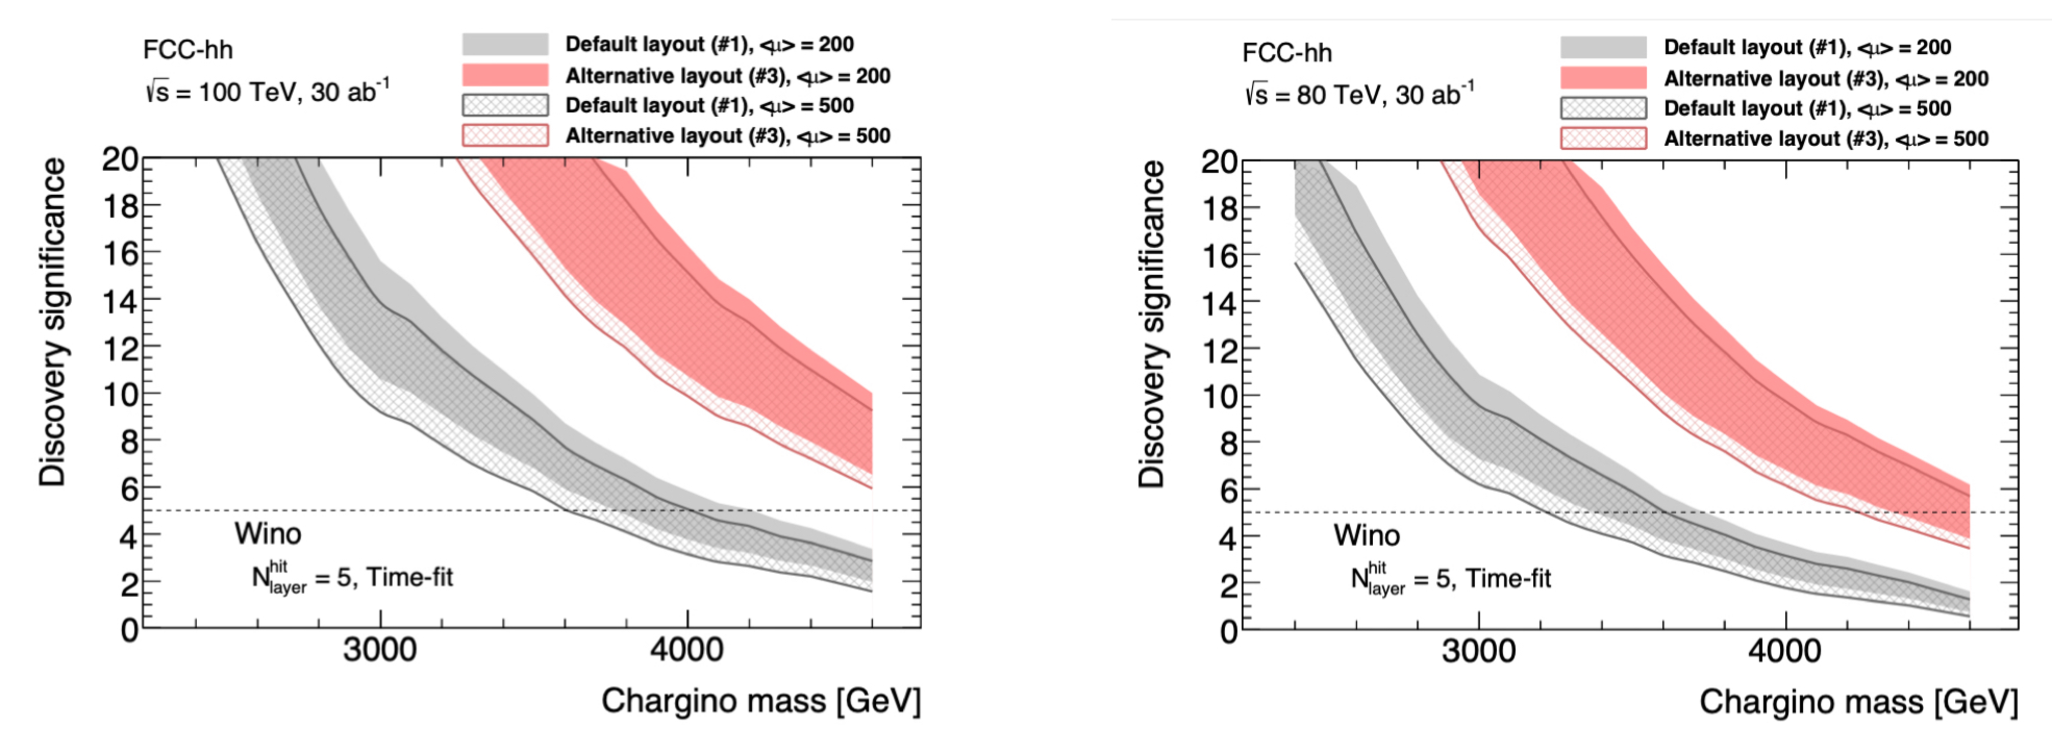
\includegraphics[width=0.98\linewidth]{PhysicsCase/Figs/wino.pdf}
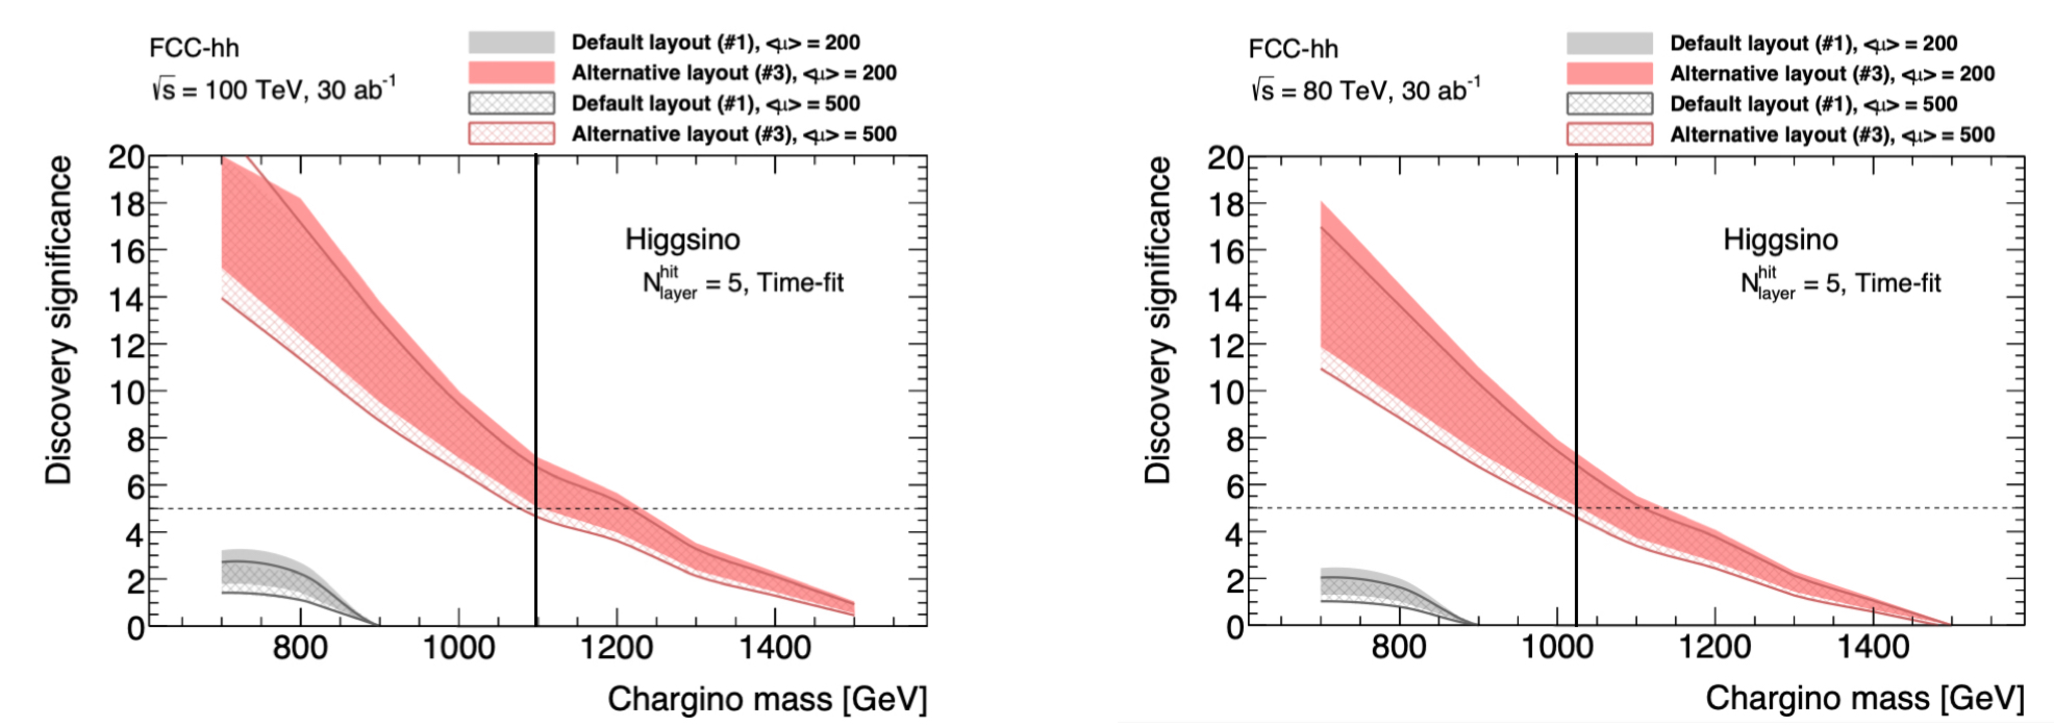
\includegraphics[width=0.98\linewidth]{PhysicsCase/Figs/higgsino.pdf} 
\caption{The 5\,$\sigma$ discovery reach for wino and higgsino dark matter candidates, 
via disappearing-track signals for $\sqrt{s} = 100$ (left) and 80\,TeV (right). 
The red band corresponds to the alternative pixel-detector layout proposed in Ref.~\cite{Saito:2019rtg}, 
where the details of the analysis are discussed.}
\label{fig:wimpdm}
\end{figure}

\subsubsection{High-mass reach}

The general potential of FCC-hh to directly explore the existence of new large-mass particles is discussed above. 
The beam energy is clearly the main driver for the mass reach. 
The detector performance and the pileup environment have a minor impact on the energy-dependence of this reach, 
a dependence that can be studied with a simple extrapolation based on the evolution with energy of the partonic luminosities, 
using, e.g., the Collider Reach tool~\cite{ColliderReach}.  
Table~\ref{tab:FCChh_sce_res} shows the extrapolation to 80 and 120\,TeV of the 5\,$\sigma$ reach 
for several possible $s$-channel resonances.
Details of the 100\,TeV analysis and the definition of the various models listed here
%
\begin{table}[ht]
\centering
\caption{Beam-energy dependence of the projected 5\,$\sigma$ discovery reach, 
with the new particle mass in TeV, for $s$-channel BSM resonances, in various decay modes. 
The definition of the various models can be found in Ref.~\cite{Helsens:2019bfw}.}
\label{tab:FCChh_sce_res}
\begin{tabular}{ l   c   c  c }
\toprule
Resonance & 100 TeV 
& 80 TeV & 120 TeV \\ 
\midrule 
Q$^*$ & 40 & 33 & 46 \\
$\PZ^\prime_\mathrm{TC2} \to \ttbar$ & 23 & 20 & 26 \\
$\PZ^\prime_\mathrm{SSM} \to \ttbar$ & 18 & 15 & 20 \\
G$_\mathrm{RS}\to \PW\PW$ & 22 & 19 & 25 \\
$\PZ^\prime_\mathrm{SSM}\to \ell\ell$ & 43 & 36 & 50 \\
$\PZ^\prime_\mathrm{SSM}\to \PGt\PGt$ & 18 & 15 & 20 \\
\bottomrule
\end{tabular}
\end{table}
%
can be found in Ref.~\cite{Helsens:2019bfw}. 
A reduction of the collision energy to 80\,TeV leads to a 15--20\% loss in mass reach, 
while running at 120\,TeV would increase the reach by 10--15\%. 
It goes without saying that, to this date, 
there is no specific model that precisely requires the existence of such new resonances in 
some of the mass ranges that would be (or not be) covered at the different energies. 
The impact of the beam-energy change is reduced for particles well below the kinematic endpoint, 
whose discovery reach is mostly limited by weak couplings, backgrounds or systematic uncertainties 
(as, for example, in the case of DM~WIMPS discussed above). 

\subsection{A forward-physics facility at FCC-hh}
\label{sec:PhysicsCaseHHFPF}

The immense breadth of the physics programme available to a hadron-collider facility is well proven by LHC, 
with its programme of $\Pp\Pp$, pN, and NN collisions (where N stands for heavy ion). 
The four large LHC experiments are accompanied by a multitude of smaller, dedicated experiments, 
which further push the exploitation of the scientific opportunities. 
A first exploration of the opportunities offered by the programme of heavy ion collisions at FCC-hh 
was presented in Ref.~\cite{Mangano:2017tke} and in the CDR~\cite{fcc-phys-cdr}. 
The additional unique opportunities that could arise from the exploitation of the high intensity beam of energetic particles, 
including neutrinos, produced by $\Pp\Pp$ collisions in the forward region, is briefly discussed here.
At LHC, these particles are studied with the far-forward experiments 
FASER($\nu$)~\cite{FASER:2020gpr,FASER:2022hcn,FASER:2023tle,FASER:2024hoe} 
and SND@LHC~\cite{SNDLHC:2022ihg,SNDLHC:2023pun}, 
and new dedicated experiments have been proposed in the context of a 
forward physics facility (FPF)~\cite{Feng:2022inv,Anchordoqui:2021ghd} operating concurrently with HL-LHC.
A FPF-like suite of far-forward experiments integrated within FCC-hh 
would provide unique opportunities for neutrino physics, QCD studies, and BSM searches.
Such FPF@FCC could be located around 1.5~km away from the IP (Fig.~\ref{fig:schematicphysics}), where a dedicated cavern would be excavated aligned with the line-of-sight (LoS).
It would have a length between 100 and 500\,m, depending on the detector setup. 
Representative applications of the FPF@FCC experiments are summarised here. 
A more detailed discussion can be found in Ref.~\cite{MammenAbraham:2024gun}.

\begin{figure}[ht]
\centering
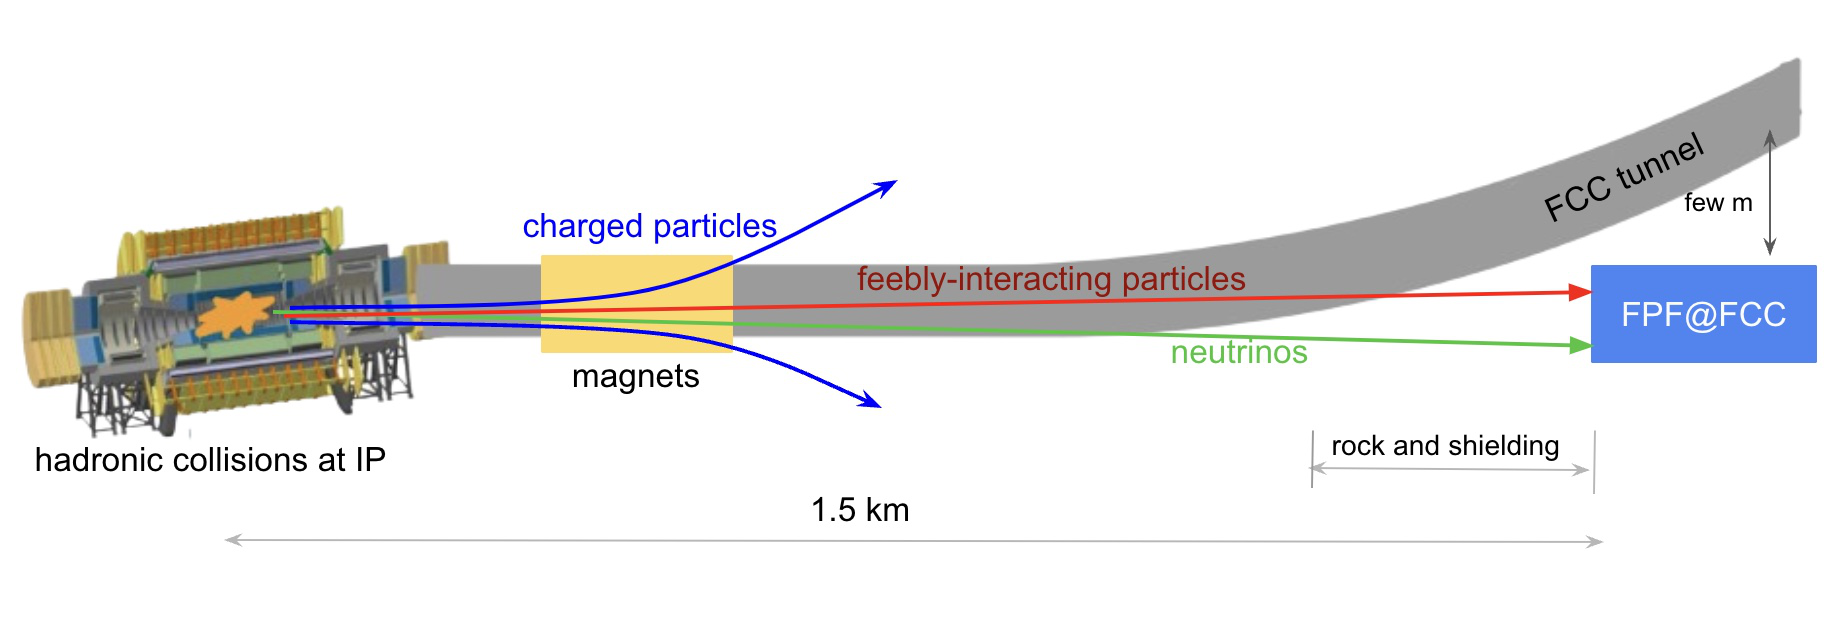
\includegraphics[width=0.8\textwidth]{PhysicsCase/Figs/FCCtunnel.png} 
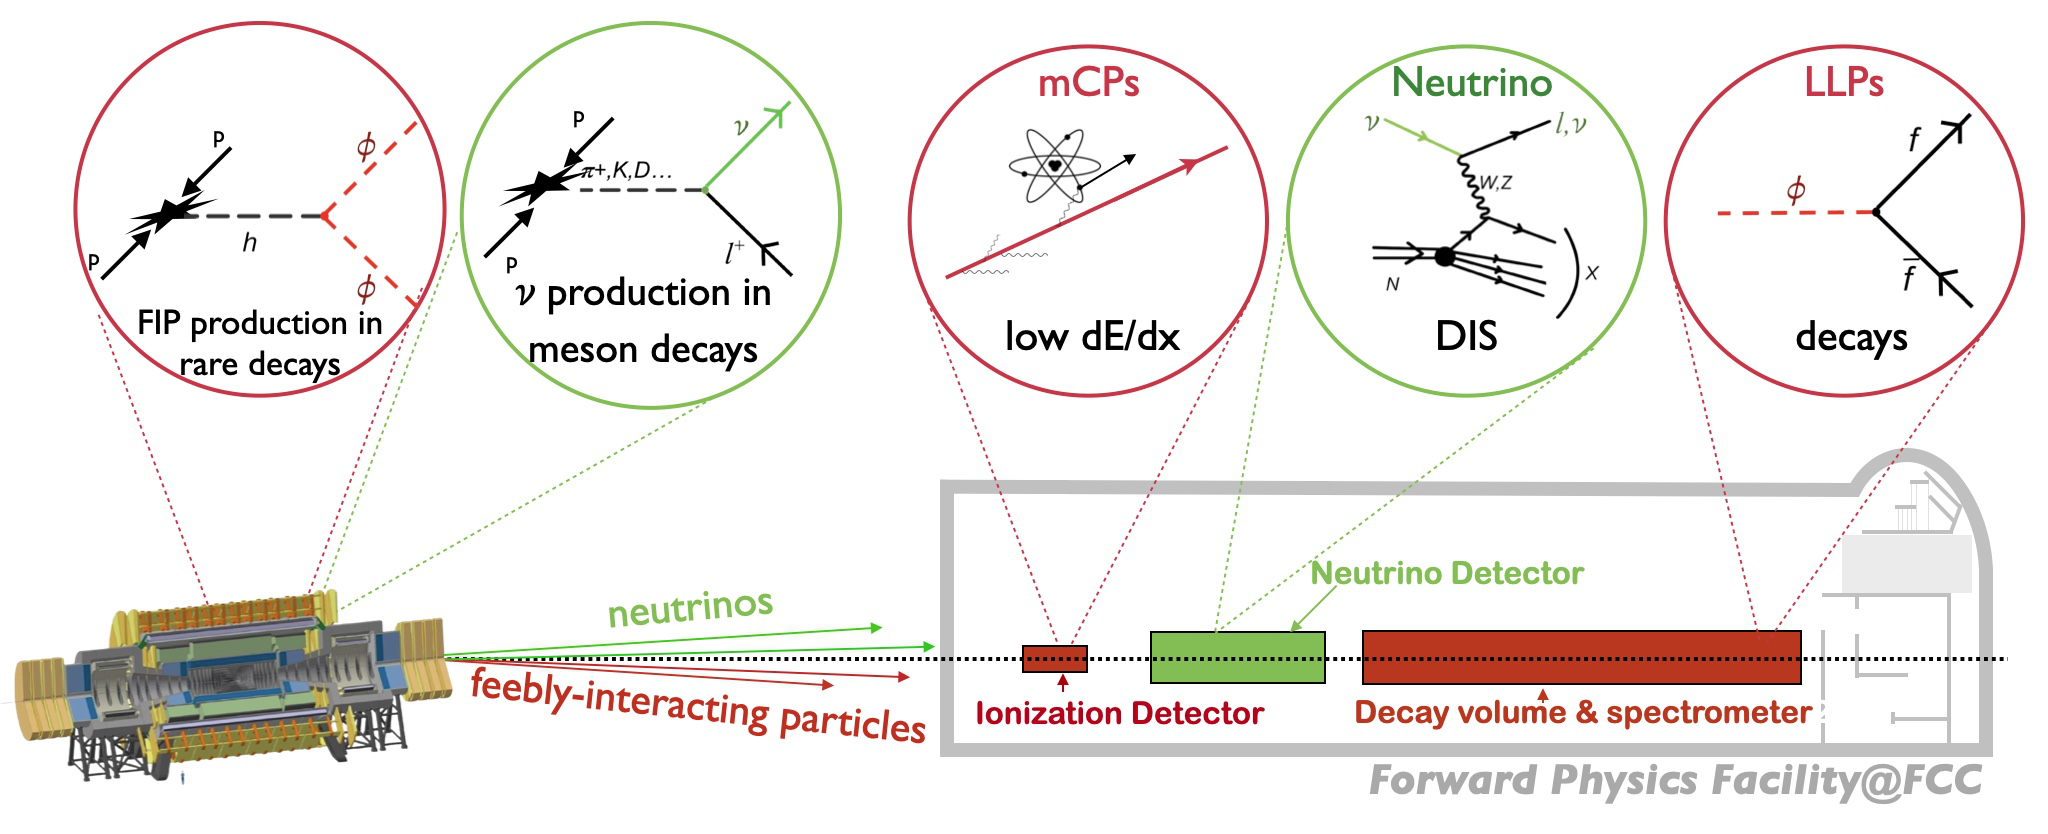
\includegraphics[width=0.8\textwidth]{PhysicsCase/Figs/FPF_final.png}
\caption{High-energy light particles (neutrinos, LLPs/FIPs) produced in FCC-hh collisions could be detected at the FPF@FCC, 
located at around 1.5\,km away from the IP, enabling sensitivity to a variety of SM and BSM signatures.}
\label{fig:schematicphysics}
\end{figure}

\subsubsection{Neutrino physics}

For neutrino detection, two options are considered:
a FASER$\PGn$2-like detector~\cite{Feng:2022inv}, dubbed FCC$\PGn$, with a length of 6.6\,m, 
and a deeper variant, FCC$\PGn$(d), with a length of 66\,m.
These detectors could collect~\cite{MammenAbraham:2024gun} up to $10^9$ electron/muon neutrinos and $10^7$ tau neutrinos 
for $\mathcal{L}_{\Pp\Pp} = 30$\,ab$^{-1}$, an increase of several orders of magnitude with respect to the (HL-)LHC yields.
These neutrinos would exhibit the highest energies ever achieved in a laboratory (up to 40\,TeV), 
overlapping with those from astrophysical sources.
The event yields forecast at the FPF@FCC would outperform all previous, ongoing, and future (proposed) neutrino experiments 
for all three generations, as indicated in Fig.~\ref{fig:fluxes-global-overview}.
These unprecedented event rates allow the precise fingerprinting of neutrino properties, 
such as their flavour universality and non-standard interactions. 

\begin{figure}[ht]
\centering
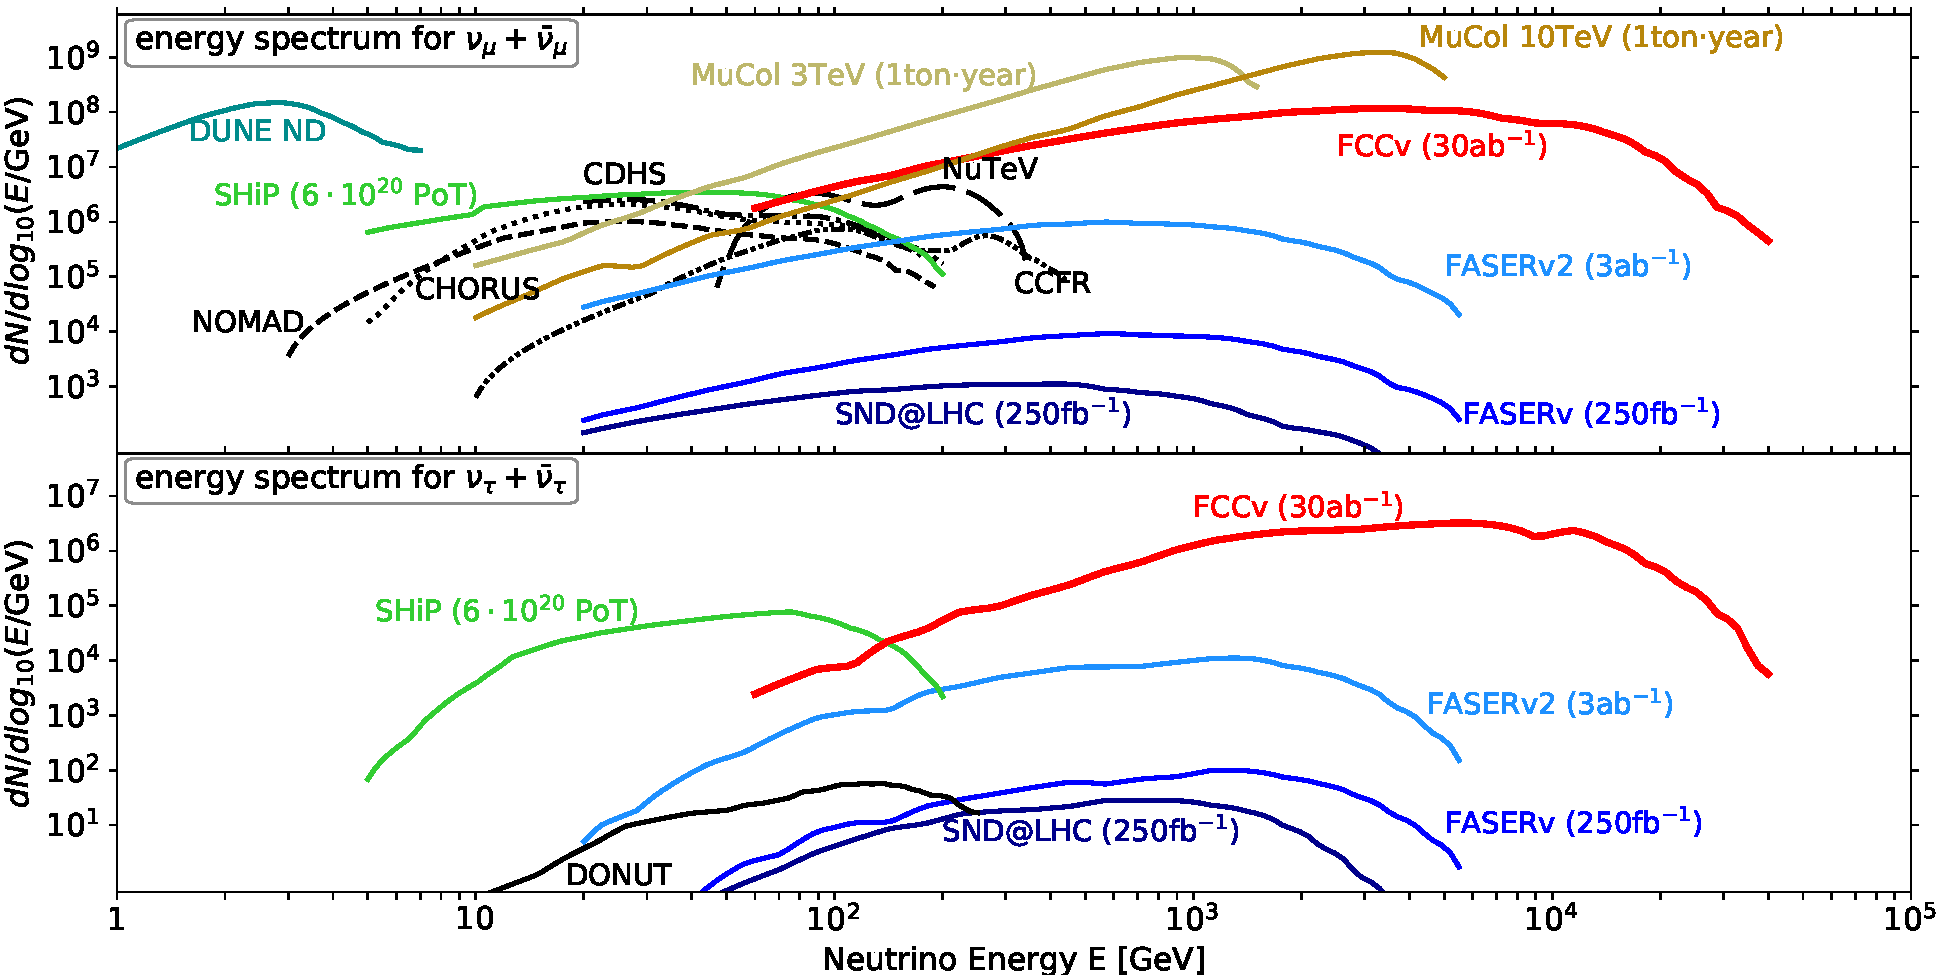
\includegraphics[width=0.9\linewidth]{PhysicsCase/Figs/NeutrinoSpectra.pdf}
\caption{The muon and tau neutrino scattering yields as a function of $E_{\PGn}$ at FCC$\PGn$ and other experiments.}
\label{fig:fluxes-global-overview}
\end{figure}

As a representative application, the electromagnetic properties of neutrinos are considered, 
long recognised as a window to new physics~\cite{Giunti:2014ixa}, 
in particular on the measurement of the neutrino charge radius $\langle r^2_{\PGn} \rangle$, 
which modifies the neutral-current DIS cross section for neutrinos.
It can be extracted~\cite{Ismail:2020yqc, MammenAbraham:2023psg} 
by searching for deviations in the ratio between NC and CC DIS events as compared to the 
$\langle r^2_{\PGn} \rangle = 0$ baseline. 
The upper left panel of Fig.~\ref{fig:BSM} shows the projected sensitivity to 
$\langle r^2_{\PGn} \rangle$ at FPF@FCC considering only statistical uncertainties.
World-leading bounds would be achieved, 
measuring the (SM) neutrino charge radius for \PGne and \PGnGm, 
and reaching down to five times the SM value for \PGnGt.
Realising this potential for precision neutrino physics 
demands an excellent modelling of CC and NC neutrino DIS interactions within the detector, 
combined with high-precision event generators for neutrino DIS~\cite{FerrarioRavasio:2024kem,Buonocore:2024pdv,vanBeekveld:2024ziz}.

\subsubsection{BSM sensitivity}

The FPF@FCC is sensitive to a variety of BSM models~\cite{MammenAbraham:2024gun}, 
including dark Higgs bosons~\cite{Kling:2021fwx}, 
relaxion-type scenarios, 
quirks~\cite{Batell:2022pzc,Li:2021tsy, Li:2023jrt, Feng:2024zgp}, 
and millicharged particles (mCPs).
These BSM signatures fall, in most cases, outside the coverage of the main FCC-hh detectors, 
and hence such a far-forward facility would markedly increase the discovery capabilities of FCC-hh.
The sensitivity to dark Higgs bosons, $\mathcal{D}$-type quirks, and mCPs of the FPF@FCC is summarised in Fig.~\ref{fig:BSM}.
The enormous rates of forward Higgs production at 100\,TeV enable the discovery of LLPs from Higgs decays 
with masses as large as 62\,GeV ($\simeq m_{\PH}/2$) 
and couplings as small as $\sin\theta \sim 10^{-8}$ (beyond the reach of FCC-ee); 
of quirks with masses up to 14\,TeV for a broad range of confinement scales $\Lambda$; 
and of mCPs with masses up to several hundreds of GeV and charge $q \sim 10^{-3} e$, 
closing the gap between (future) accelerator-based bounds and dark matter direct detection searches.

\begin{figure}[ht]
\centering
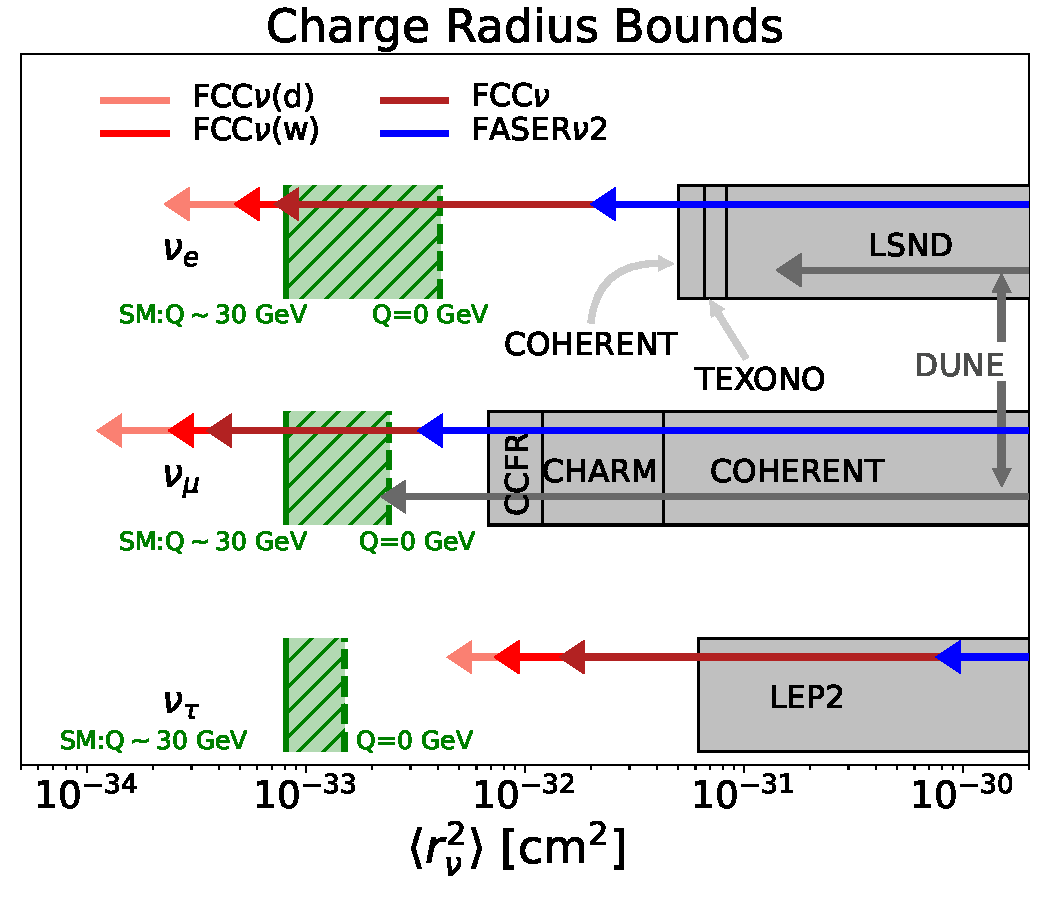
\includegraphics[width=0.4\textwidth]{PhysicsCase/Figs/final_results_chradius_binned.pdf} 
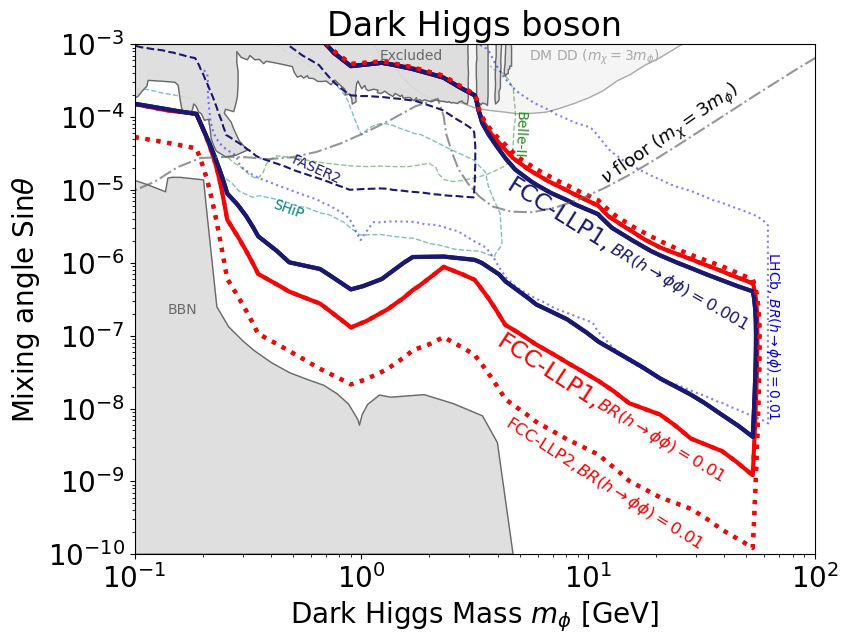
\includegraphics[width=0.45\textwidth]{PhysicsCase/Figs/HiggsPortal1.png}
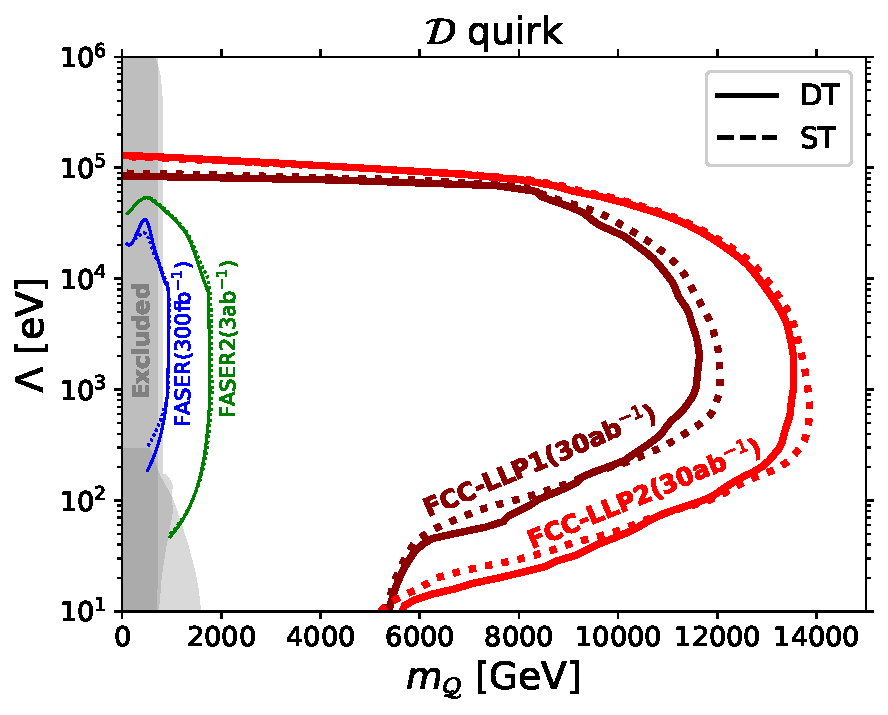
\includegraphics[width=0.45\textwidth]{PhysicsCase/Figs/cont_f33_fcc.pdf}
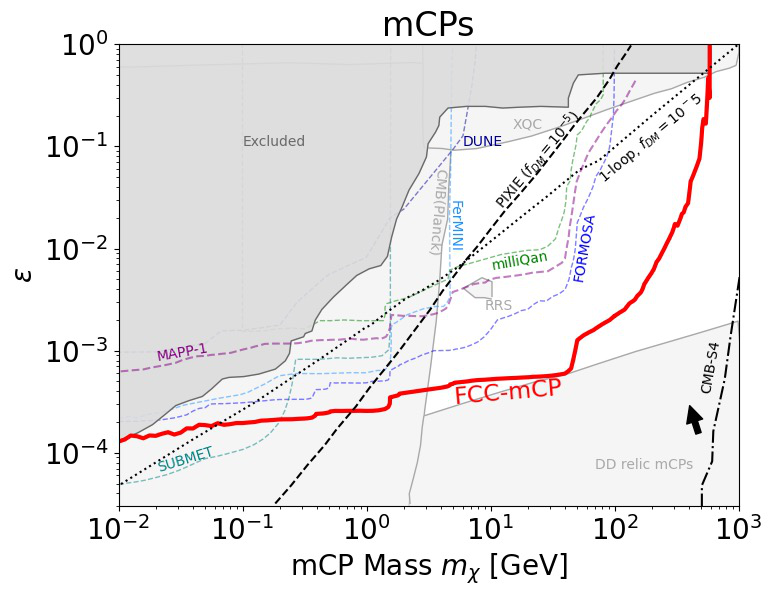
\includegraphics[width=0.45\textwidth]{PhysicsCase/Figs/mCP.png}
\caption{Top left: Sensitivity of the FCC$\PGn$ detectors to the neutrino charge radius.
Top right: Reach for a dark Higgs boson $\phi$ at the FPF@FCC.
Bottom left: Discovery potential for $\mathcal{D}$-type quirks with mass $m_{\mathcal{Q}}$ and confinement scale $\Lambda$. 
Bottom right: Sensitivity to mCPs with mixing parameter $\epsilon$.} 
\label{fig:BSM}
\end{figure}

\subsubsection{QCD and hadronic structure}

The enormous samples of multi-TeV neutrinos available at the FPF@FCC (Fig.~\ref{fig:fluxes-global-overview}) 
enable high-resolution probes of the unpolarised and polarised structure of protons and of heavy nuclei, 
as summarised by the representative applications of Fig.~\ref{fig:QCD}.

\begin{figure}[ht]
\centering
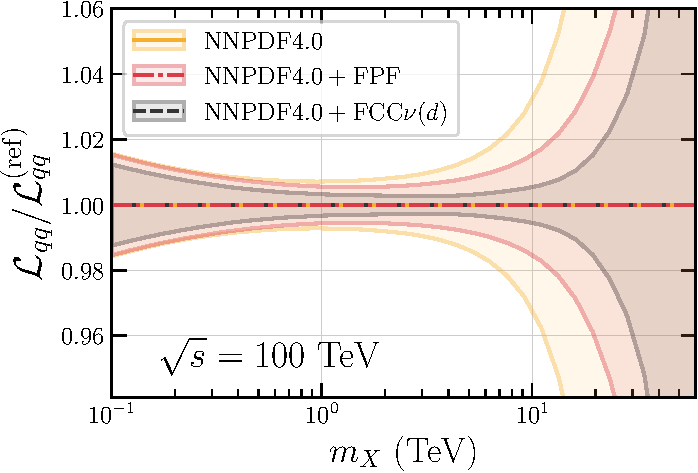
\includegraphics[width=0.3\textwidth]{PhysicsCase/Figs/lumi-FCCnu-summary.pdf} 
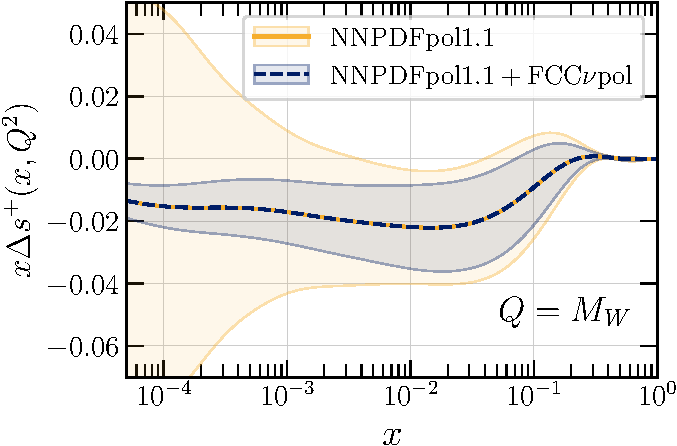
\includegraphics[width=0.3\textwidth]{PhysicsCase/Figs/PolarisedPDFs-RW-summary.pdf}  
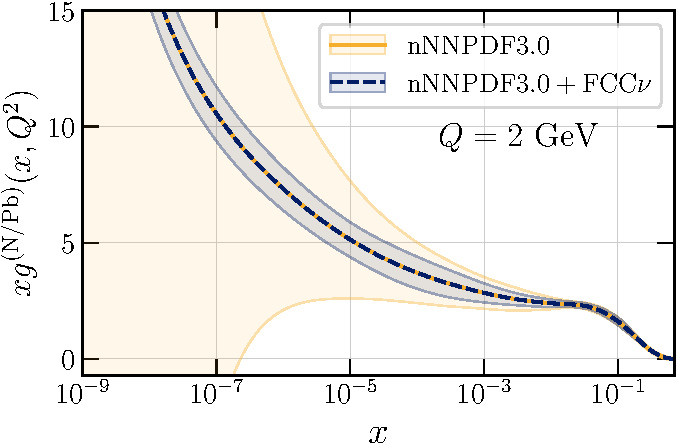
\includegraphics[width=0.3\textwidth]{PhysicsCase/Figs/NuclearPDFs-RW-summary.pdf}  
\caption{Projected constraints from the FPF@FCC experiments on 
the unpolarised (left) and polarised (middle) PDFs, 
and on the nuclear PDFs of lead nuclei (right).}
\label{fig:QCD}
\end{figure}

First, high-energy neutrino DIS structure functions~\cite{Cruz-Martinez:2023sdv,Candido:2023utz} 
provide a precise quark/antiquark flavour separation at large-$x$, 
which in turn reduces the theoretical uncertainties entering high-mass searches at FCC-hh.
Second, neutrino DIS on a polarised target~\cite{Forte:2001ph,Mangano:2001mj} 
resolves the spin structure of the proton~\cite{Nocera:2014gqa,Borsa:2024mss} 
with complementary information to related experiments, 
such as those at the Electron-Ion Collider~\cite{AbdulKhalek:2021gbh}.
Third, detecting neutrinos originating from proton-lead collisions provides 
information on nuclear structure~\cite{Klasen:2023uqj,Eskola:2021nhw,AbdulKhalek:2022fyi} down to $x \sim 10^{-9}$, 
where nuclear PDFs are unconstrained and novel dynamical regimes of QCD, 
such as the Colour Glass Condensate, are expected to dominate.
This kinematic region is also of prime importance for astroparticle physics experiments.

\subsubsection{Summary}

Integrating far-forward experiments into FCC-hh would extend its scientific potential 
in several synergetic directions from QCD and neutrino physics to BSM searches in a cost-efficient manner.
While at this early stage no attempt has been made to optimise the accelerator infrastructure 
or define the FPF@FCC detector technology more precisely, 
the results shown here motivate further studies of how to fully realise this unique physics potential.
